\documentclass[12pt, a4paper]{article}
\usepackage[romanian]{babel}
\usepackage{hyperref}
\usepackage{physics}
\usepackage{amsmath}
\usepackage{tikz}
\usepackage{mathdots}
\usepackage{yhmath}
\usepackage{cancel}
\usepackage{color}
\usepackage{siunitx}
\usepackage{array}
\usepackage{multirow}
\usepackage{amssymb}
\usepackage{gensymb}
\usepackage{tabularx}
\usepackage{extarrows}
\usepackage{booktabs}
\usetikzlibrary{fadings}
\usetikzlibrary{patterns}
\usetikzlibrary{shadows.blur}
\usetikzlibrary{shapes}
\usepackage{fancyhdr}
\usepackage{graphicx}
\usepackage{amsmath}
\usepackage{multirow}
\usepackage{array}

\renewcommand{\arraystretch}{1.5}
\hypersetup{%
    pdfborder = {0 0 0}
}

\DeclareGraphicsExtensions{.pdf,.png}

\title{\centering{Electrotehnica în profunzime\\
                    Tema de casă}}
\author{\textbf{Negru Mihai}\\
        Grupa 313CD, Anul 1\\
        email \href{mailto:mihai.upb.info2021@gmail.com}{mihai.upb.info2021@gmail.com}\\
        Universitatea Politehnica București\\
        Facultatea de Automatică și Calculatoare\\
        Calculatoare și Tehnologiile Informației}

\date{Mai 2022}

\pagestyle{fancy}
\fancyhf{}
\rhead{Negru Mihai}
\lhead{Universitatea Politehnica din București}
\cfoot{\thepage}

\begin{document}

\maketitle
\newpage
\tableofcontents{}
\newpage

\section{Generarea unui circuit}
Vom începe prin a reprezenta schemetic un graf conex care va reprezenta circuitul electric rezistiv liniar.
\tikzset{every picture/.style={line width=0.75pt}} %set default line width to 0.75pt        

\begin{center}
    \begin{tikzpicture}[x=0.75pt,y=0.75pt,yscale=-1,xscale=1]
    
    %uncomment if require: \path (0,300); %set diagram left start at 0, and has height of 300
    
    %Shape: Rectangle [id:dp632185373066857] 
    \draw   (57,47) -- (611,47) -- (611,265.05) -- (57,265.05) -- cycle ;
    %Straight Lines [id:da21045800549237814] 
    \draw    (443,266.05) -- (441,46.05) ;
    %Straight Lines [id:da004890146660028849] 
    \draw    (240,46.05) -- (240,265.05) ;
    %Straight Lines [id:da9436228030524887] 
    \draw    (57,47) -- (240,155.55) ;
    %Straight Lines [id:da5807636430233452] 
    \draw    (57,265.05) -- (240,155.55) ;
    %Straight Lines [id:da07520304550863566] 
    \draw    (610,157.5) -- (442,156.05) ;
    %Shape: Circle [id:dp8908991627382346] 
    \draw  [fill={rgb, 255:red, 14; green, 13; blue, 13 }  ,fill opacity=1 ] (50.52,48.76) .. controls (50.52,46.16) and (52.63,44.05) .. (55.24,44.05) .. controls (57.84,44.05) and (59.95,46.16) .. (59.95,48.76) .. controls (59.95,51.37) and (57.84,53.48) .. (55.24,53.48) .. controls (52.63,53.48) and (50.52,51.37) .. (50.52,48.76) -- cycle ;
    %Shape: Circle [id:dp11473877397988663] 
    \draw  [fill={rgb, 255:red, 14; green, 13; blue, 13 }  ,fill opacity=1 ] (52.29,265.05) .. controls (52.29,262.44) and (54.4,260.33) .. (57,260.33) .. controls (59.6,260.33) and (61.71,262.44) .. (61.71,265.05) .. controls (61.71,267.65) and (59.6,269.76) .. (57,269.76) .. controls (54.4,269.76) and (52.29,267.65) .. (52.29,265.05) -- cycle ;
    %Shape: Circle [id:dp5807254321001776] 
    \draw  [fill={rgb, 255:red, 14; green, 13; blue, 13 }  ,fill opacity=1 ] (235.29,155.55) .. controls (235.29,152.94) and (237.4,150.83) .. (240,150.83) .. controls (242.6,150.83) and (244.71,152.94) .. (244.71,155.55) .. controls (244.71,158.15) and (242.6,160.26) .. (240,160.26) .. controls (237.4,160.26) and (235.29,158.15) .. (235.29,155.55) -- cycle ;
    %Shape: Circle [id:dp3646520570999061] 
    \draw  [fill={rgb, 255:red, 14; green, 13; blue, 13 }  ,fill opacity=1 ] (235.29,50.76) .. controls (235.29,48.16) and (237.4,46.05) .. (240,46.05) .. controls (242.6,46.05) and (244.71,48.16) .. (244.71,50.76) .. controls (244.71,53.37) and (242.6,55.48) .. (240,55.48) .. controls (237.4,55.48) and (235.29,53.37) .. (235.29,50.76) -- cycle ;
    %Shape: Circle [id:dp5825982820045075] 
    \draw  [fill={rgb, 255:red, 14; green, 13; blue, 13 }  ,fill opacity=1 ] (235.29,265.05) .. controls (235.29,262.44) and (237.4,260.33) .. (240,260.33) .. controls (242.6,260.33) and (244.71,262.44) .. (244.71,265.05) .. controls (244.71,267.65) and (242.6,269.76) .. (240,269.76) .. controls (237.4,269.76) and (235.29,267.65) .. (235.29,265.05) -- cycle ;
    %Shape: Circle [id:dp14863797103649068] 
    \draw  [fill={rgb, 255:red, 14; green, 13; blue, 13 }  ,fill opacity=1 ] (437.29,156.05) .. controls (437.29,153.44) and (439.4,151.33) .. (442,151.33) .. controls (444.6,151.33) and (446.71,153.44) .. (446.71,156.05) .. controls (446.71,158.65) and (444.6,160.76) .. (442,160.76) .. controls (439.4,160.76) and (437.29,158.65) .. (437.29,156.05) -- cycle ;
    %Shape: Circle [id:dp6624636049301356] 
    \draw  [fill={rgb, 255:red, 14; green, 13; blue, 13 }  ,fill opacity=1 ] (436.29,50.76) .. controls (436.29,48.16) and (438.4,46.05) .. (441,46.05) .. controls (443.6,46.05) and (445.71,48.16) .. (445.71,50.76) .. controls (445.71,53.37) and (443.6,55.48) .. (441,55.48) .. controls (438.4,55.48) and (436.29,53.37) .. (436.29,50.76) -- cycle ;
    %Shape: Circle [id:dp09770898595203037] 
    \draw  [fill={rgb, 255:red, 14; green, 13; blue, 13 }  ,fill opacity=1 ] (438.29,266.05) .. controls (438.29,263.44) and (440.4,261.33) .. (443,261.33) .. controls (445.6,261.33) and (447.71,263.44) .. (447.71,266.05) .. controls (447.71,268.65) and (445.6,270.76) .. (443,270.76) .. controls (440.4,270.76) and (438.29,268.65) .. (438.29,266.05) -- cycle ;
    %Shape: Circle [id:dp24800518053003495] 
    \draw  [fill={rgb, 255:red, 14; green, 13; blue, 13 }  ,fill opacity=1 ] (605.29,157.5) .. controls (605.29,154.9) and (607.4,152.79) .. (610,152.79) .. controls (612.6,152.79) and (614.71,154.9) .. (614.71,157.5) .. controls (614.71,160.1) and (612.6,162.21) .. (610,162.21) .. controls (607.4,162.21) and (605.29,160.1) .. (605.29,157.5) -- cycle ;
    
    \end{tikzpicture}
\end{center}
Observăm că topologia grafului de mai sus este:
\begin{itemize}
    \item Numarul de noduri: \textbf{9}
    \item Numarul de laturi: \textbf{14}
    \item Numarul de secțiuni fundamentale: \textbf{8}
    \item Numarul de bucle fundamentale: \textbf{6}
\end{itemize}
În cele ce urmează vom căuta un arbore pentru graful desenat mai sus pentru a putea inițializa lucrul cu intensitățile și tensiunile circuitului.

\begin{center}
    \tikzset{every picture/.style={line width=0.75pt}} %set default line width to 0.75pt        
    
    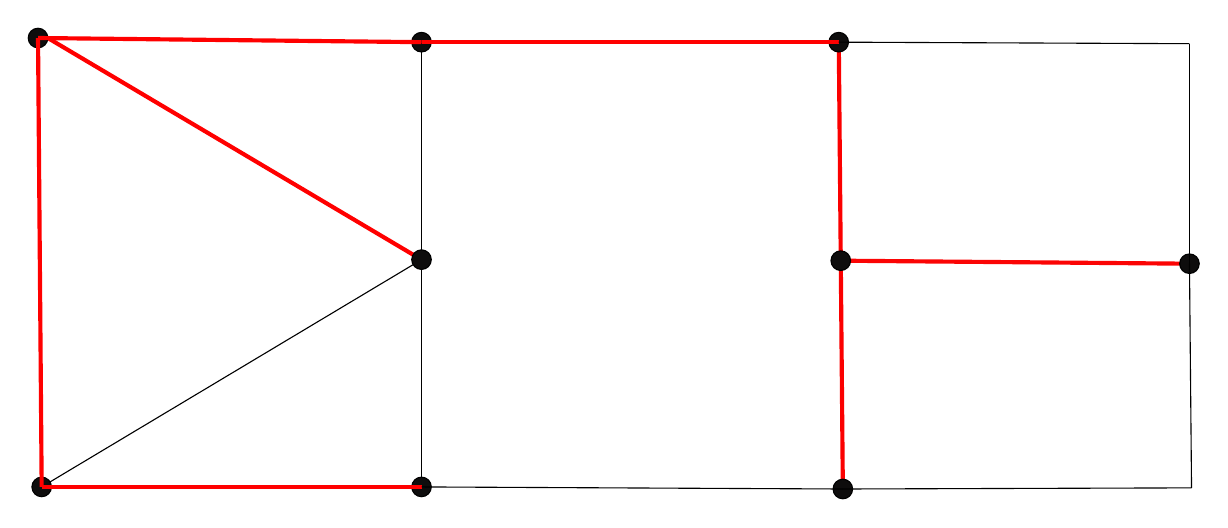
\begin{tikzpicture}[x=0.75pt,y=0.75pt,yscale=-1,xscale=1]
    %uncomment if require: \path (0,300); %set diagram left start at 0, and has height of 300
    
    %Straight Lines [id:da21045800549237814] 
    \draw [color={rgb, 255:red, 251; green, 0; blue, 0 }  ,draw opacity=1 ][line width=1.5]    (443,266.05) -- (441,46.05) ;
    %Straight Lines [id:da004890146660028849] 
    \draw    (240,46.05) -- (240,265.05) ;
    %Straight Lines [id:da9436228030524887] 
    \draw [color={rgb, 255:red, 255; green, 0; blue, 0 }  ,draw opacity=1 ][line width=1.5]    (57,47) -- (240,155.55) ;
    %Straight Lines [id:da5807636430233452] 
    \draw    (57,265.05) -- (240,155.55) ;
    %Straight Lines [id:da07520304550863566] 
    \draw [color={rgb, 255:red, 251; green, 4; blue, 4 }  ,draw opacity=1 ][line width=1.5]    (610,157.5) -- (442,156.05) ;
    %Shape: Circle [id:dp8908991627382346] 
    \draw  [fill={rgb, 255:red, 14; green, 13; blue, 13 }  ,fill opacity=1 ] (50.52,48.76) .. controls (50.52,46.16) and (52.63,44.05) .. (55.24,44.05) .. controls (57.84,44.05) and (59.95,46.16) .. (59.95,48.76) .. controls (59.95,51.37) and (57.84,53.48) .. (55.24,53.48) .. controls (52.63,53.48) and (50.52,51.37) .. (50.52,48.76) -- cycle ;
    %Shape: Circle [id:dp11473877397988663] 
    \draw  [fill={rgb, 255:red, 14; green, 13; blue, 13 }  ,fill opacity=1 ] (52.29,265.05) .. controls (52.29,262.44) and (54.4,260.33) .. (57,260.33) .. controls (59.6,260.33) and (61.71,262.44) .. (61.71,265.05) .. controls (61.71,267.65) and (59.6,269.76) .. (57,269.76) .. controls (54.4,269.76) and (52.29,267.65) .. (52.29,265.05) -- cycle ;
    %Shape: Circle [id:dp5807254321001776] 
    \draw  [fill={rgb, 255:red, 14; green, 13; blue, 13 }  ,fill opacity=1 ] (235.29,155.55) .. controls (235.29,152.94) and (237.4,150.83) .. (240,150.83) .. controls (242.6,150.83) and (244.71,152.94) .. (244.71,155.55) .. controls (244.71,158.15) and (242.6,160.26) .. (240,160.26) .. controls (237.4,160.26) and (235.29,158.15) .. (235.29,155.55) -- cycle ;
    %Shape: Circle [id:dp3646520570999061] 
    \draw  [fill={rgb, 255:red, 14; green, 13; blue, 13 }  ,fill opacity=1 ] (235.29,50.76) .. controls (235.29,48.16) and (237.4,46.05) .. (240,46.05) .. controls (242.6,46.05) and (244.71,48.16) .. (244.71,50.76) .. controls (244.71,53.37) and (242.6,55.48) .. (240,55.48) .. controls (237.4,55.48) and (235.29,53.37) .. (235.29,50.76) -- cycle ;
    %Shape: Circle [id:dp5825982820045075] 
    \draw  [fill={rgb, 255:red, 14; green, 13; blue, 13 }  ,fill opacity=1 ] (235.29,265.05) .. controls (235.29,262.44) and (237.4,260.33) .. (240,260.33) .. controls (242.6,260.33) and (244.71,262.44) .. (244.71,265.05) .. controls (244.71,267.65) and (242.6,269.76) .. (240,269.76) .. controls (237.4,269.76) and (235.29,267.65) .. (235.29,265.05) -- cycle ;
    %Shape: Circle [id:dp14863797103649068] 
    \draw  [fill={rgb, 255:red, 14; green, 13; blue, 13 }  ,fill opacity=1 ] (437.29,156.05) .. controls (437.29,153.44) and (439.4,151.33) .. (442,151.33) .. controls (444.6,151.33) and (446.71,153.44) .. (446.71,156.05) .. controls (446.71,158.65) and (444.6,160.76) .. (442,160.76) .. controls (439.4,160.76) and (437.29,158.65) .. (437.29,156.05) -- cycle ;
    %Shape: Circle [id:dp6624636049301356] 
    \draw  [fill={rgb, 255:red, 14; green, 13; blue, 13 }  ,fill opacity=1 ] (436.29,50.76) .. controls (436.29,48.16) and (438.4,46.05) .. (441,46.05) .. controls (443.6,46.05) and (445.71,48.16) .. (445.71,50.76) .. controls (445.71,53.37) and (443.6,55.48) .. (441,55.48) .. controls (438.4,55.48) and (436.29,53.37) .. (436.29,50.76) -- cycle ;
    %Shape: Circle [id:dp09770898595203037] 
    \draw  [fill={rgb, 255:red, 14; green, 13; blue, 13 }  ,fill opacity=1 ] (438.29,266.05) .. controls (438.29,263.44) and (440.4,261.33) .. (443,261.33) .. controls (445.6,261.33) and (447.71,263.44) .. (447.71,266.05) .. controls (447.71,268.65) and (445.6,270.76) .. (443,270.76) .. controls (440.4,270.76) and (438.29,268.65) .. (438.29,266.05) -- cycle ;
    %Shape: Circle [id:dp24800518053003495] 
    \draw  [fill={rgb, 255:red, 14; green, 13; blue, 13 }  ,fill opacity=1 ] (605.29,157.5) .. controls (605.29,154.9) and (607.4,152.79) .. (610,152.79) .. controls (612.6,152.79) and (614.71,154.9) .. (614.71,157.5) .. controls (614.71,160.1) and (612.6,162.21) .. (610,162.21) .. controls (607.4,162.21) and (605.29,160.1) .. (605.29,157.5) -- cycle ;
    %Straight Lines [id:da616679450964865] 
    \draw [color={rgb, 255:red, 255; green, 0; blue, 0 }  ,draw opacity=1 ][line width=1.5]    (55.24,48.76) -- (240,50.76) ;
    %Straight Lines [id:da45712321633467745] 
    \draw [color={rgb, 255:red, 255; green, 0; blue, 0 }  ,draw opacity=1 ][fill={rgb, 255:red, 255; green, 0; blue, 0 }  ,fill opacity=1 ][line width=1.5]    (55.24,48.76) -- (57,265.05) ;
    %Straight Lines [id:da7071492325225306] 
    \draw [color={rgb, 255:red, 255; green, 0; blue, 0 }  ,draw opacity=1 ][line width=1.5]    (57,265.05) -- (240,265.05) ;
    %Straight Lines [id:da5617837683084317] 
    \draw [color={rgb, 255:red, 255; green, 0; blue, 0 }  ,draw opacity=1 ][line width=1.5]    (240,50.76) -- (441,50.76) ;
    %Straight Lines [id:da7099031494228125] 
    \draw    (443,266.05) -- (240,265.05) ;
    %Straight Lines [id:da2756686295424895] 
    \draw    (610,51.5) -- (441,50.76) ;
    %Straight Lines [id:da9904378794079685] 
    \draw    (610,51.5) -- (610,157.5) ;
    %Straight Lines [id:da3335504328107153] 
    \draw    (611,265.5) -- (443,266.05) ;
    %Straight Lines [id:da3656330988117984] 
    \draw    (611,265.5) -- (610,157.5) ;
    \end{tikzpicture}
\end{center}
\newpage

Un arbore va trece prin toate nodurile grafului și nu va avea cicluri în componența acestuia astfel numărul total de ramuri va fi egal cu numărul de secțiuni fundamentale adică \textbf{8}.

În continuare vom stabili 2 grafuri cel de tensiune și cel de curenți. Pentru a păstra proprietatea de bună formulare a unui circuit vom predefini pentru ramurile arborelui tensiuni \textbf{aleatoare}, iar pentru coarde tensiunea se va afla cu \textbf{Kirchfoff II}. Pentru intensități vom predefini valori \textbf{aleatoare} pe coardele grafului, iar pentru ramuri insensitățile se vor afla cu \textbf{Kirchhoff I}.

\begin{center}


\tikzset{every picture/.style={line width=0.75pt}} %set default line width to 0.75pt        

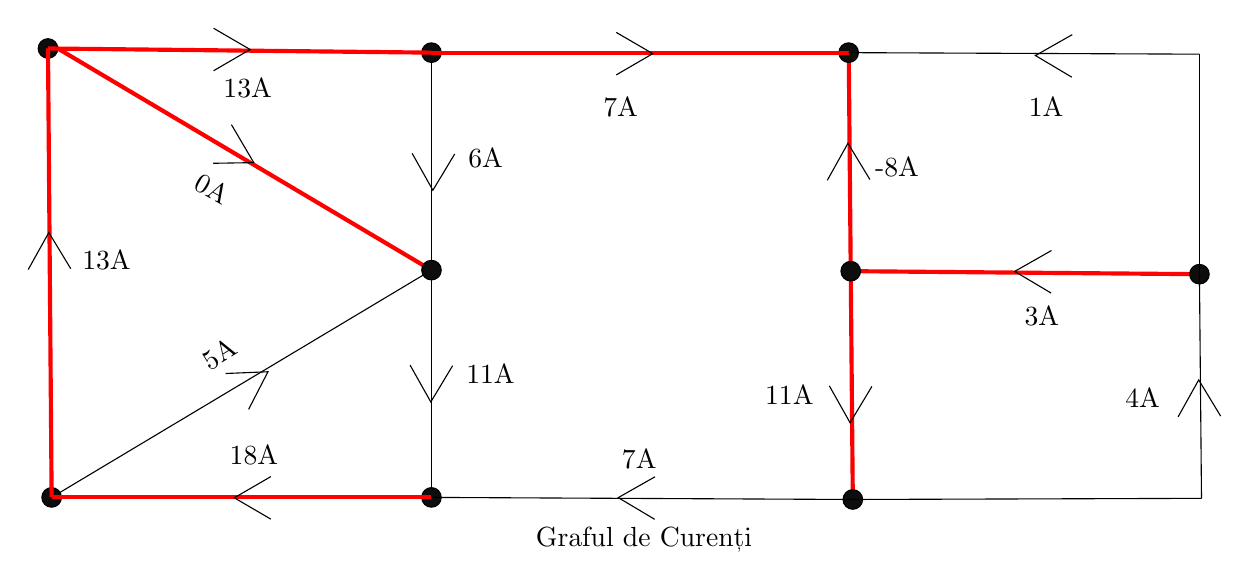
\begin{tikzpicture}[x=0.75pt,y=0.75pt,yscale=-1,xscale=1]
%uncomment if require: \path (0,300); %set diagram left start at 0, and has height of 300

%Straight Lines [id:da21045800549237814] 
\draw [color={rgb, 255:red, 251; green, 0; blue, 0 }  ,draw opacity=1 ][line width=1.5]    (443,266.05) -- (441,46.05) ;
%Straight Lines [id:da004890146660028849] 
\draw    (240,46.05) -- (240,265.05) ;
%Straight Lines [id:da9436228030524887] 
\draw [color={rgb, 255:red, 255; green, 0; blue, 0 }  ,draw opacity=1 ][line width=1.5]    (57,47) -- (240,155.55) ;
%Straight Lines [id:da5807636430233452] 
\draw    (57,265.05) -- (240,155.55) ;
%Straight Lines [id:da07520304550863566] 
\draw [color={rgb, 255:red, 251; green, 4; blue, 4 }  ,draw opacity=1 ][line width=1.5]    (610,157.5) -- (442,156.05) ;
%Shape: Circle [id:dp8908991627382346] 
\draw  [fill={rgb, 255:red, 14; green, 13; blue, 13 }  ,fill opacity=1 ] (50.52,48.76) .. controls (50.52,46.16) and (52.63,44.05) .. (55.24,44.05) .. controls (57.84,44.05) and (59.95,46.16) .. (59.95,48.76) .. controls (59.95,51.37) and (57.84,53.48) .. (55.24,53.48) .. controls (52.63,53.48) and (50.52,51.37) .. (50.52,48.76) -- cycle ;
%Shape: Circle [id:dp11473877397988663] 
\draw  [fill={rgb, 255:red, 14; green, 13; blue, 13 }  ,fill opacity=1 ] (52.29,265.05) .. controls (52.29,262.44) and (54.4,260.33) .. (57,260.33) .. controls (59.6,260.33) and (61.71,262.44) .. (61.71,265.05) .. controls (61.71,267.65) and (59.6,269.76) .. (57,269.76) .. controls (54.4,269.76) and (52.29,267.65) .. (52.29,265.05) -- cycle ;
%Shape: Circle [id:dp5807254321001776] 
\draw  [fill={rgb, 255:red, 14; green, 13; blue, 13 }  ,fill opacity=1 ] (235.29,155.55) .. controls (235.29,152.94) and (237.4,150.83) .. (240,150.83) .. controls (242.6,150.83) and (244.71,152.94) .. (244.71,155.55) .. controls (244.71,158.15) and (242.6,160.26) .. (240,160.26) .. controls (237.4,160.26) and (235.29,158.15) .. (235.29,155.55) -- cycle ;
%Shape: Circle [id:dp3646520570999061] 
\draw  [fill={rgb, 255:red, 14; green, 13; blue, 13 }  ,fill opacity=1 ] (235.29,50.76) .. controls (235.29,48.16) and (237.4,46.05) .. (240,46.05) .. controls (242.6,46.05) and (244.71,48.16) .. (244.71,50.76) .. controls (244.71,53.37) and (242.6,55.48) .. (240,55.48) .. controls (237.4,55.48) and (235.29,53.37) .. (235.29,50.76) -- cycle ;
%Shape: Circle [id:dp5825982820045075] 
\draw  [fill={rgb, 255:red, 14; green, 13; blue, 13 }  ,fill opacity=1 ] (235.29,265.05) .. controls (235.29,262.44) and (237.4,260.33) .. (240,260.33) .. controls (242.6,260.33) and (244.71,262.44) .. (244.71,265.05) .. controls (244.71,267.65) and (242.6,269.76) .. (240,269.76) .. controls (237.4,269.76) and (235.29,267.65) .. (235.29,265.05) -- cycle ;
%Shape: Circle [id:dp14863797103649068] 
\draw  [fill={rgb, 255:red, 14; green, 13; blue, 13 }  ,fill opacity=1 ] (437.29,156.05) .. controls (437.29,153.44) and (439.4,151.33) .. (442,151.33) .. controls (444.6,151.33) and (446.71,153.44) .. (446.71,156.05) .. controls (446.71,158.65) and (444.6,160.76) .. (442,160.76) .. controls (439.4,160.76) and (437.29,158.65) .. (437.29,156.05) -- cycle ;
%Shape: Circle [id:dp6624636049301356] 
\draw  [fill={rgb, 255:red, 14; green, 13; blue, 13 }  ,fill opacity=1 ] (436.29,50.76) .. controls (436.29,48.16) and (438.4,46.05) .. (441,46.05) .. controls (443.6,46.05) and (445.71,48.16) .. (445.71,50.76) .. controls (445.71,53.37) and (443.6,55.48) .. (441,55.48) .. controls (438.4,55.48) and (436.29,53.37) .. (436.29,50.76) -- cycle ;
%Shape: Circle [id:dp09770898595203037] 
\draw  [fill={rgb, 255:red, 14; green, 13; blue, 13 }  ,fill opacity=1 ] (438.29,266.05) .. controls (438.29,263.44) and (440.4,261.33) .. (443,261.33) .. controls (445.6,261.33) and (447.71,263.44) .. (447.71,266.05) .. controls (447.71,268.65) and (445.6,270.76) .. (443,270.76) .. controls (440.4,270.76) and (438.29,268.65) .. (438.29,266.05) -- cycle ;
%Shape: Circle [id:dp24800518053003495] 
\draw  [fill={rgb, 255:red, 14; green, 13; blue, 13 }  ,fill opacity=1 ] (605.29,157.5) .. controls (605.29,154.9) and (607.4,152.79) .. (610,152.79) .. controls (612.6,152.79) and (614.71,154.9) .. (614.71,157.5) .. controls (614.71,160.1) and (612.6,162.21) .. (610,162.21) .. controls (607.4,162.21) and (605.29,160.1) .. (605.29,157.5) -- cycle ;
%Straight Lines [id:da616679450964865] 
\draw [color={rgb, 255:red, 255; green, 0; blue, 0 }  ,draw opacity=1 ][line width=1.5]    (55.24,48.76) -- (240,50.76) ;
%Straight Lines [id:da45712321633467745] 
\draw [color={rgb, 255:red, 255; green, 0; blue, 0 }  ,draw opacity=1 ][fill={rgb, 255:red, 255; green, 0; blue, 0 }  ,fill opacity=1 ][line width=1.5]    (55.24,48.76) -- (57,265.05) ;
%Straight Lines [id:da7071492325225306] 
\draw [color={rgb, 255:red, 255; green, 0; blue, 0 }  ,draw opacity=1 ][line width=1.5]    (57,265.05) -- (240,265.05) ;
%Straight Lines [id:da5617837683084317] 
\draw [color={rgb, 255:red, 255; green, 0; blue, 0 }  ,draw opacity=1 ][line width=1.5]    (240,50.76) -- (441,50.76) ;
%Straight Lines [id:da7099031494228125] 
\draw    (443,266.05) -- (240,265.05) ;
%Straight Lines [id:da2756686295424895] 
\draw    (610,51.5) -- (441,50.76) ;
%Straight Lines [id:da9904378794079685] 
\draw    (610,51.5) -- (610,157.5) ;
%Straight Lines [id:da3335504328107153] 
\draw    (611,265.5) -- (443,266.05) ;
%Straight Lines [id:da3656330988117984] 
\draw    (611,265.5) -- (610,157.5) ;
\draw   (135,39) -- (152.62,49.25) -- (135,59.5) ;
\draw   (143.61,85.43) -- (154.38,103.75) -- (134.86,104.07) ;
\draw   (45.72,155.25) -- (55.65,137.44) -- (66.22,154.87) ;
\draw   (140.87,205.35) -- (161.23,204.51) -- (151.9,222.63) ;
\draw   (162.61,275.51) -- (145,265.24) -- (162.63,255.01) ;
\draw   (251.19,99.6) -- (240.68,117.06) -- (230.69,99.29) ;
\draw   (250.19,201.6) -- (239.68,219.06) -- (229.69,201.29) ;
\draw   (329,41) -- (346.62,51.25) -- (329,61.5) ;
\draw   (430.72,112.25) -- (440.65,94.44) -- (451.22,111.87) ;
\draw   (452.19,211.6) -- (441.68,229.06) -- (431.69,211.29) ;
\draw   (538.52,166.59) -- (521,156.16) -- (538.72,146.09) ;
\draw   (599.72,226.25) -- (609.65,208.44) -- (620.22,225.87) ;
\draw   (548.52,62.59) -- (531,52.16) -- (548.72,42.09) ;
\draw   (347.52,275.59) -- (330,265.16) -- (347.72,255.09) ;

% Text Node
\draw (157,67.75) node   [align=left] {\begin{minipage}[lt]{25.84pt}\setlength\topsep{0pt}
13A
\end{minipage}};
% Text Node
\draw (89,150.75) node   [align=left] {\begin{minipage}[lt]{25.84pt}\setlength\topsep{0pt}
13A
\end{minipage}};
% Text Node
\draw (145.29,191.22) node  [rotate=-328.16] [align=left] {\begin{minipage}[lt]{25.84pt}\setlength\topsep{0pt}
5A
\end{minipage}};
% Text Node
\draw (274,205.75) node   [align=left] {\begin{minipage}[lt]{25.84pt}\setlength\topsep{0pt}
11A
\end{minipage}};
% Text Node
\draw (160,244.75) node   [align=left] {\begin{minipage}[lt]{25.84pt}\setlength\topsep{0pt}
18A
\end{minipage}};
% Text Node
\draw (142,120.75) node  [rotate=-29.47] [align=left] {\begin{minipage}[lt]{25.84pt}\setlength\topsep{0pt}
0A
\end{minipage}};
% Text Node
\draw (275,101.75) node   [align=left] {\begin{minipage}[lt]{25.84pt}\setlength\topsep{0pt}
6A
\end{minipage}};
% Text Node
\draw (340,76.75) node   [align=left] {\begin{minipage}[lt]{25.84pt}\setlength\topsep{0pt}
7A
\end{minipage}};
% Text Node
\draw (545,76.75) node   [align=left] {\begin{minipage}[lt]{25.84pt}\setlength\topsep{0pt}
1A
\end{minipage}};
% Text Node
\draw (471,105.75) node   [align=left] {\begin{minipage}[lt]{25.84pt}\setlength\topsep{0pt}
\mbox{-}8A
\end{minipage}};
% Text Node
\draw (349,246.75) node   [align=left] {\begin{minipage}[lt]{25.84pt}\setlength\topsep{0pt}
7A
\end{minipage}};
% Text Node
\draw (418,215.75) node   [align=left] {\begin{minipage}[lt]{25.84pt}\setlength\topsep{0pt}
11A
\end{minipage}};
% Text Node
\draw (591.5,217.25) node   [align=left] {\begin{minipage}[lt]{25.84pt}\setlength\topsep{0pt}
4A
\end{minipage}};
% Text Node
\draw (543,177.75) node   [align=left] {\begin{minipage}[lt]{25.84pt}\setlength\topsep{0pt}
3A
\end{minipage}};
% Text Node
\draw (289,278) node [anchor=north west][inner sep=0.75pt]   [align=left] {Graful de Curenți};


\end{tikzpicture}

\end{center}

\begin{center}


\tikzset{every picture/.style={line width=0.75pt}} %set default line width to 0.75pt        

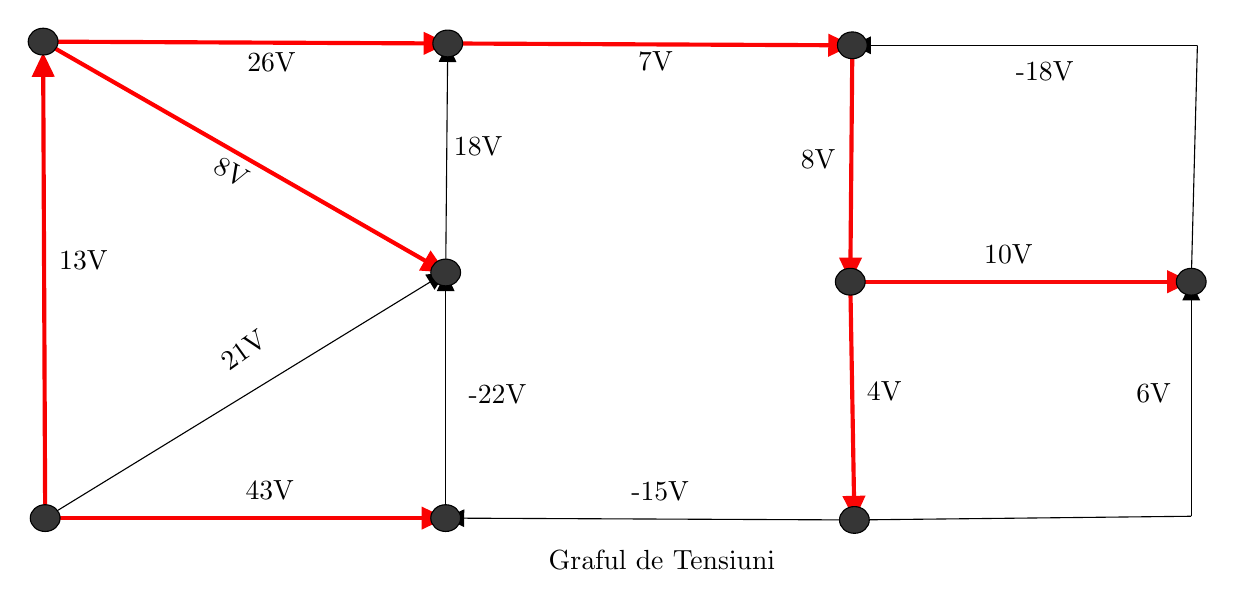
\begin{tikzpicture}[x=0.75pt,y=0.75pt,yscale=-1,xscale=1]
%uncomment if require: \path (0,300); %set diagram left start at 0, and has height of 300

%Straight Lines [id:da2007473758909839] 
\draw [color={rgb, 255:red, 254; green, 0; blue, 0 }  ,draw opacity=1 ][line width=1.5]    (44.01,19.28) -- (234.95,20.16) ;
\draw [shift={(238.95,20.17)}, rotate = 180.26] [fill={rgb, 255:red, 254; green, 0; blue, 0 }  ,fill opacity=1 ][line width=0.08]  [draw opacity=0] (11.61,-5.58) -- (0,0) -- (11.61,5.58) -- cycle    ;
%Straight Lines [id:da5805126599838257] 
\draw [color={rgb, 255:red, 247; green, 0; blue, 0 }  ,draw opacity=1 ][line width=1.5]    (45,248.85) -- (44.03,28.62) ;
\draw [shift={(44.01,24.62)}, rotate = 89.75] [fill={rgb, 255:red, 247; green, 0; blue, 0 }  ,fill opacity=1 ][line width=0.08]  [draw opacity=0] (11.61,-5.58) -- (0,0) -- (11.61,5.58) -- cycle    ;
%Straight Lines [id:da8738581165107147] 
\draw [color={rgb, 255:red, 249; green, 2; blue, 2 }  ,draw opacity=1 ][line width=1.5]    (45,248.85) -- (233.96,248.85) ;
\draw [shift={(237.96,248.85)}, rotate = 180] [fill={rgb, 255:red, 249; green, 2; blue, 2 }  ,fill opacity=1 ][line width=0.08]  [draw opacity=0] (11.61,-5.58) -- (0,0) -- (11.61,5.58) -- cycle    ;
%Straight Lines [id:da8246688638523951] 
\draw    (237.96,130.51) -- (238.92,23.17) ;
\draw [shift={(238.95,20.17)}, rotate = 90.51] [fill={rgb, 255:red, 0; green, 0; blue, 0 }  ][line width=0.08]  [draw opacity=0] (8.93,-4.29) -- (0,0) -- (8.93,4.29) -- cycle    ;
%Straight Lines [id:da1596653387550402] 
\draw    (237.96,248.85) -- (237.96,133.51) ;
\draw [shift={(237.96,130.51)}, rotate = 90] [fill={rgb, 255:red, 0; green, 0; blue, 0 }  ][line width=0.08]  [draw opacity=0] (8.93,-4.29) -- (0,0) -- (8.93,4.29) -- cycle    ;
%Straight Lines [id:da5555019763907534] 
\draw [color={rgb, 255:red, 255; green, 0; blue, 0 }  ,draw opacity=1 ][line width=1.5]    (44.01,19.28) -- (234.49,128.52) ;
\draw [shift={(237.96,130.51)}, rotate = 209.83] [fill={rgb, 255:red, 255; green, 0; blue, 0 }  ,fill opacity=1 ][line width=0.08]  [draw opacity=0] (11.61,-5.58) -- (0,0) -- (11.61,5.58) -- cycle    ;
%Straight Lines [id:da1584487637276637] 
\draw    (45,248.85) -- (235.4,132.08) ;
\draw [shift={(237.96,130.51)}, rotate = 148.48] [fill={rgb, 255:red, 0; green, 0; blue, 0 }  ][line width=0.08]  [draw opacity=0] (8.93,-4.29) -- (0,0) -- (8.93,4.29) -- cycle    ;
%Straight Lines [id:da07384074659043027] 
\draw [color={rgb, 255:red, 252; green, 4; blue, 4 }  ,draw opacity=1 ][line width=1.5]    (238.95,20.17) -- (429.89,21.05) ;
\draw [shift={(433.89,21.06)}, rotate = 180.26] [fill={rgb, 255:red, 252; green, 4; blue, 4 }  ,fill opacity=1 ][line width=0.08]  [draw opacity=0] (11.61,-5.58) -- (0,0) -- (11.61,5.58) -- cycle    ;
%Straight Lines [id:da6237409008125407] 
\draw    (434.87,249.74) -- (240.96,248.86) ;
\draw [shift={(237.96,248.85)}, rotate = 0.26] [fill={rgb, 255:red, 0; green, 0; blue, 0 }  ][line width=0.08]  [draw opacity=0] (8.93,-4.29) -- (0,0) -- (8.93,4.29) -- cycle    ;
%Straight Lines [id:da9464008767654883] 
\draw [color={rgb, 255:red, 247; green, 5; blue, 5 }  ,draw opacity=1 ][line width=1.5]    (433.89,21.06) -- (432.93,130.96) ;
\draw [shift={(432.9,134.96)}, rotate = 270.5] [fill={rgb, 255:red, 247; green, 5; blue, 5 }  ,fill opacity=1 ][line width=0.08]  [draw opacity=0] (11.61,-5.58) -- (0,0) -- (11.61,5.58) -- cycle    ;
%Straight Lines [id:da7590611938251033] 
\draw [color={rgb, 255:red, 251; green, 6; blue, 6 }  ,draw opacity=1 ][line width=1.5]    (432.9,134.96) -- (434.81,245.74) ;
\draw [shift={(434.87,249.74)}, rotate = 269.01] [fill={rgb, 255:red, 251; green, 6; blue, 6 }  ,fill opacity=1 ][line width=0.08]  [draw opacity=0] (11.61,-5.58) -- (0,0) -- (11.61,5.58) -- cycle    ;
%Straight Lines [id:da8684739282858722] 
\draw [color={rgb, 255:red, 249; green, 9; blue, 9 }  ,draw opacity=1 ][line width=1.5]    (432.9,134.96) -- (593.16,134.96) ;
\draw [shift={(597.16,134.96)}, rotate = 180] [fill={rgb, 255:red, 249; green, 9; blue, 9 }  ,fill opacity=1 ][line width=0.08]  [draw opacity=0] (11.61,-5.58) -- (0,0) -- (11.61,5.58) -- cycle    ;
%Straight Lines [id:da08465928321582727] 
\draw    (600.13,21.06) -- (436.89,21.06) ;
\draw [shift={(433.89,21.06)}, rotate = 360] [fill={rgb, 255:red, 0; green, 0; blue, 0 }  ][line width=0.08]  [draw opacity=0] (8.93,-4.29) -- (0,0) -- (8.93,4.29) -- cycle    ;
%Straight Lines [id:da07742523144624669] 
\draw    (600.13,21.06) -- (597.16,134.96) ;
%Straight Lines [id:da8674741768771632] 
\draw    (597.16,247.96) -- (597.16,137.96) ;
\draw [shift={(597.16,134.96)}, rotate = 90] [fill={rgb, 255:red, 0; green, 0; blue, 0 }  ][line width=0.08]  [draw opacity=0] (8.93,-4.29) -- (0,0) -- (8.93,4.29) -- cycle    ;
%Straight Lines [id:da3035074751642657] 
\draw    (434.87,249.74) -- (597.16,247.96) ;
%Shape: Ellipse [id:dp702105646651815] 
\draw  [fill={rgb, 255:red, 54; green, 54; blue, 54 }  ,fill opacity=1 ] (426.71,21.06) .. controls (426.71,17.5) and (429.92,14.61) .. (433.89,14.61) .. controls (437.85,14.61) and (441.06,17.5) .. (441.06,21.06) .. controls (441.06,24.63) and (437.85,27.51) .. (433.89,27.51) .. controls (429.92,27.51) and (426.71,24.63) .. (426.71,21.06) -- cycle ;
%Shape: Ellipse [id:dp20532633875874495] 
\draw  [fill={rgb, 255:red, 54; green, 54; blue, 54 }  ,fill opacity=1 ] (425.72,134.96) .. controls (425.72,131.39) and (428.93,128.51) .. (432.9,128.51) .. controls (436.86,128.51) and (440.07,131.39) .. (440.07,134.96) .. controls (440.07,138.52) and (436.86,141.41) .. (432.9,141.41) .. controls (428.93,141.41) and (425.72,138.52) .. (425.72,134.96) -- cycle ;
%Shape: Ellipse [id:dp7688627874216465] 
\draw  [fill={rgb, 255:red, 54; green, 54; blue, 54 }  ,fill opacity=1 ] (589.99,134.96) .. controls (589.99,131.39) and (593.2,128.51) .. (597.16,128.51) .. controls (601.12,128.51) and (604.33,131.39) .. (604.33,134.96) .. controls (604.33,138.52) and (601.12,141.41) .. (597.16,141.41) .. controls (593.2,141.41) and (589.99,138.52) .. (589.99,134.96) -- cycle ;
%Shape: Ellipse [id:dp4237078330938182] 
\draw  [fill={rgb, 255:red, 54; green, 54; blue, 54 }  ,fill opacity=1 ] (427.7,249.74) .. controls (427.7,246.18) and (430.91,243.29) .. (434.87,243.29) .. controls (438.84,243.29) and (442.05,246.18) .. (442.05,249.74) .. controls (442.05,253.3) and (438.84,256.19) .. (434.87,256.19) .. controls (430.91,256.19) and (427.7,253.3) .. (427.7,249.74) -- cycle ;
%Shape: Ellipse [id:dp9547436642438543] 
\draw  [fill={rgb, 255:red, 54; green, 54; blue, 54 }  ,fill opacity=1 ] (231.77,20.17) .. controls (231.77,16.61) and (234.98,13.72) .. (238.95,13.72) .. controls (242.91,13.72) and (246.12,16.61) .. (246.12,20.17) .. controls (246.12,23.74) and (242.91,26.63) .. (238.95,26.63) .. controls (234.98,26.63) and (231.77,23.74) .. (231.77,20.17) -- cycle ;
%Shape: Ellipse [id:dp7949325370928308] 
\draw  [fill={rgb, 255:red, 54; green, 54; blue, 54 }  ,fill opacity=1 ] (230.78,130.51) .. controls (230.78,126.95) and (233.99,124.06) .. (237.96,124.06) .. controls (241.92,124.06) and (245.13,126.95) .. (245.13,130.51) .. controls (245.13,134.07) and (241.92,136.96) .. (237.96,136.96) .. controls (233.99,136.96) and (230.78,134.07) .. (230.78,130.51) -- cycle ;
%Shape: Ellipse [id:dp44539204376449804] 
\draw  [fill={rgb, 255:red, 54; green, 54; blue, 54 }  ,fill opacity=1 ] (230.78,248.85) .. controls (230.78,245.29) and (233.99,242.4) .. (237.96,242.4) .. controls (241.92,242.4) and (245.13,245.29) .. (245.13,248.85) .. controls (245.13,252.41) and (241.92,255.3) .. (237.96,255.3) .. controls (233.99,255.3) and (230.78,252.41) .. (230.78,248.85) -- cycle ;
%Shape: Ellipse [id:dp21768997242867516] 
\draw  [fill={rgb, 255:red, 54; green, 54; blue, 54 }  ,fill opacity=1 ] (37.82,248.85) .. controls (37.82,245.29) and (41.03,242.4) .. (45,242.4) .. controls (48.96,242.4) and (52.17,245.29) .. (52.17,248.85) .. controls (52.17,252.41) and (48.96,255.3) .. (45,255.3) .. controls (41.03,255.3) and (37.82,252.41) .. (37.82,248.85) -- cycle ;
%Shape: Ellipse [id:dp5490196740132514] 
\draw  [fill={rgb, 255:red, 54; green, 54; blue, 54 }  ,fill opacity=1 ] (36.83,19.28) .. controls (36.83,15.72) and (40.05,12.83) .. (44.01,12.83) .. controls (47.97,12.83) and (51.18,15.72) .. (51.18,19.28) .. controls (51.18,22.85) and (47.97,25.74) .. (44.01,25.74) .. controls (40.05,25.74) and (36.83,22.85) .. (36.83,19.28) -- cycle ;

% Text Node
\draw (141.1,23.42) node [anchor=north west][inner sep=0.75pt]   [align=left] {26V};
% Text Node
\draw (50.49,118.47) node [anchor=north west][inner sep=0.75pt]   [align=left] {13V};
% Text Node
\draw (129.35,72.04) node [anchor=north west][inner sep=0.75pt]  [rotate=-29.97] [align=left] {8V};
% Text Node
\draw (126.61,170.68) node [anchor=north west][inner sep=0.75pt]  [rotate=-324.47] [align=left] {21V};
% Text Node
\draw (140.28,229.66) node [anchor=north west][inner sep=0.75pt]   [align=left] {43V};
% Text Node
\draw (247.77,183.42) node [anchor=north west][inner sep=0.75pt]   [align=left] {\mbox{-}22V};
% Text Node
\draw (240.68,63.79) node [anchor=north west][inner sep=0.75pt]   [align=left] {18V};
% Text Node
\draw (329.46,23.05) node [anchor=north west][inner sep=0.75pt]   [align=left] {7V};
% Text Node
\draw (326.13,230.03) node [anchor=north west][inner sep=0.75pt]   [align=left] {\mbox{-}15V};
% Text Node
\draw (439.65,181.59) node [anchor=north west][inner sep=0.75pt]   [align=left] {4V};
% Text Node
\draw (569.44,182.69) node [anchor=north west][inner sep=0.75pt]   [align=left] {6V};
% Text Node
\draw (407.82,70.02) node [anchor=north west][inner sep=0.75pt]   [align=left] {8V};
% Text Node
\draw (511.42,27.82) node [anchor=north west][inner sep=0.75pt]   [align=left] {\mbox{-}18V};
% Text Node
\draw (496.17,115.9) node [anchor=north west][inner sep=0.75pt]   [align=left] {10V};
% Text Node
\draw (286.33,263.06) node [anchor=north west][inner sep=0.75pt]   [align=left] {Graful de Tensiuni};


\end{tikzpicture}
\end{center}

\newpage

Pentru a verifica acum dacă graful de curenți și graful de tensiuni este bine construit vom verifica \emph{Legea lui Tellegen}.
$$P_c = 13\cdot26 + 7\cdot7 - 1\cdot18 + 0\cdot8 + 13\cdot13 + 21\cdot5 - 15\cdot7 + 4\cdot11 + 4\cdot6$$
$$P_g = 43\cdot18 - 22\cdot11 + 18\cdot6 - 8\cdot8 + 3\cdot10$$
Cum $P_c = P_g = 606W \Rightarrow$ că \emph{Legea lui Tellegen} este verificată și putem să mergem la pasul următor de construcție a unui circuit electric liniar rezistiv.

\begin{center}


\tikzset{every picture/.style={line width=0.75pt}} %set default line width to 0.75pt        

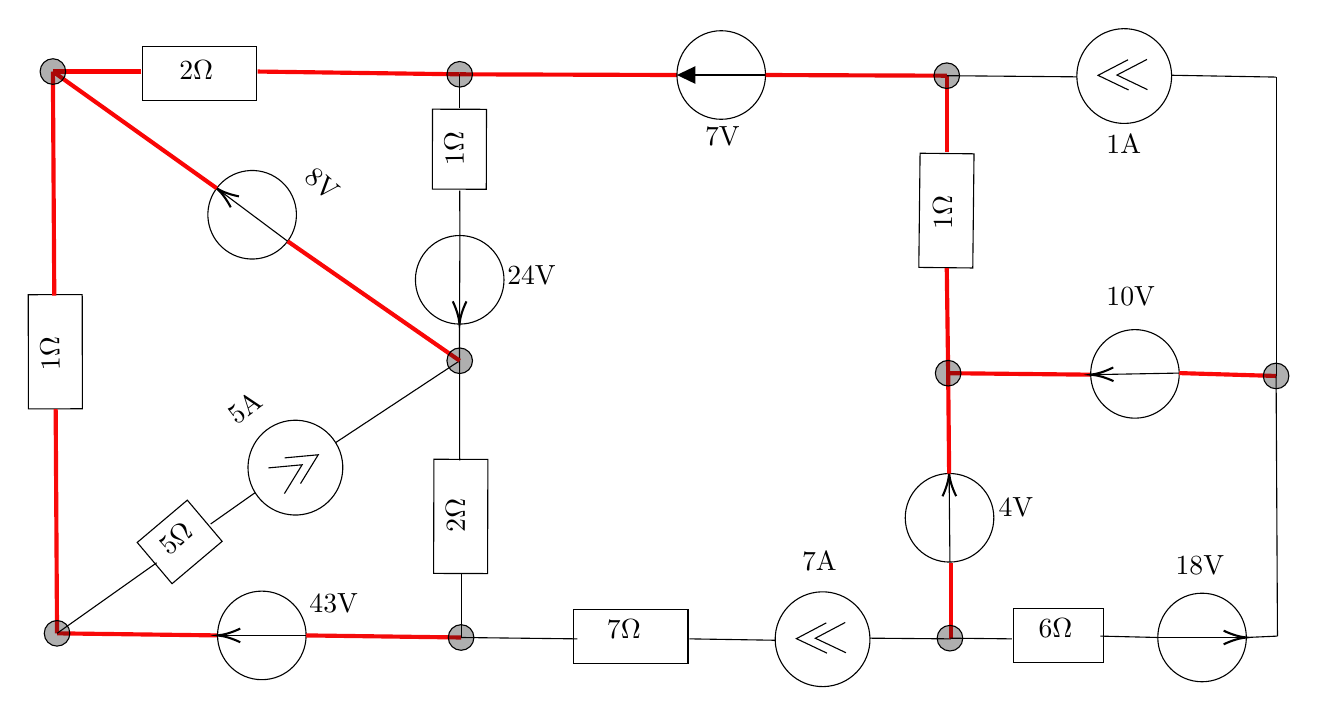
\begin{tikzpicture}[x=0.75pt,y=0.75pt,yscale=-1,xscale=1]
%uncomment if require: \path (0,470); %set diagram left start at 0, and has height of 470

%Flowchart: Connector [id:dp3210958141129272] 
\draw   (554.67,365.67) .. controls (554.67,353.88) and (564.22,344.33) .. (576,344.33) .. controls (587.78,344.33) and (597.33,353.88) .. (597.33,365.67) .. controls (597.33,377.45) and (587.78,387) .. (576,387) .. controls (564.22,387) and (554.67,377.45) .. (554.67,365.67) -- cycle ;
%Straight Lines [id:da07866549022195546] 
\draw    (554.67,365.67) -- (595.33,365.67) ;
\draw [shift={(597.33,365.67)}, rotate = 180] [color={rgb, 255:red, 0; green, 0; blue, 0 }  ][line width=0.75]    (10.93,-3.29) .. controls (6.95,-1.4) and (3.31,-0.3) .. (0,0) .. controls (3.31,0.3) and (6.95,1.4) .. (10.93,3.29)   ;

%Shape: Rectangle [id:dp0733903504183755] 
\draw   (485.33,351.67) -- (528.33,351.67) -- (528.33,377.67) -- (485.33,377.67) -- cycle ;
%Shape: Rectangle [id:dp815014661772993] 
\draw   (65.33,81) -- (120.33,81) -- (120.33,107) -- (65.33,107) -- cycle ;
%Straight Lines [id:da3447478282084555] 
\draw [color={rgb, 255:red, 249; green, 2; blue, 2 }  ,draw opacity=1 ][line width=1.5]    (65,93) -- (22.33,93) ;
%Shape: Rectangle [id:dp6563430844169236] 
\draw   (36.45,200.48) -- (36.55,255.48) -- (10.55,255.52) -- (10.45,200.52) -- cycle ;
%Straight Lines [id:da5780959071676919] 
\draw [color={rgb, 255:red, 249; green, 7; blue, 7 }  ,draw opacity=1 ][line width=1.5]    (22.33,93) -- (23,201) ;
%Straight Lines [id:da5720390620758491] 
\draw [color={rgb, 255:red, 249; green, 10; blue, 10 }  ,draw opacity=1 ][line width=1.5]    (23.67,255.67) -- (24.33,363.67) ;
%Straight Lines [id:da7033452915585461] 
\draw [color={rgb, 255:red, 249; green, 9; blue, 9 }  ,draw opacity=1 ][line width=1.5]    (24.33,363.67) -- (101.67,364.67) ;
%Flowchart: Connector [id:dp07523236477311368] 
\draw   (144.33,364.67) .. controls (144.33,376.45) and (134.78,386) .. (123,386) .. controls (111.22,386) and (101.67,376.45) .. (101.67,364.67) .. controls (101.67,352.88) and (111.22,343.33) .. (123,343.33) .. controls (134.78,343.33) and (144.33,352.88) .. (144.33,364.67) -- cycle ;
%Straight Lines [id:da4040766459348697] 
\draw    (144.33,364.67) -- (103.67,364.67) ;
\draw [shift={(101.67,364.67)}, rotate = 360] [color={rgb, 255:red, 0; green, 0; blue, 0 }  ][line width=0.75]    (10.93,-3.29) .. controls (6.95,-1.4) and (3.31,-0.3) .. (0,0) .. controls (3.31,0.3) and (6.95,1.4) .. (10.93,3.29)   ;

%Straight Lines [id:da15036978699151526] 
\draw [color={rgb, 255:red, 244; green, 11; blue, 11 }  ,draw opacity=1 ][line width=1.5]    (219,365.67) -- (144.33,364.67) ;
%Straight Lines [id:da09841377869386081] 
\draw [color={rgb, 255:red, 249; green, 6; blue, 6 }  ,draw opacity=1 ][line width=1.5]    (121,93) -- (218.33,94.33) ;
%Straight Lines [id:da41036930721590803] 
\draw    (219,335) -- (219,365.67) ;
%Shape: Rectangle [id:dp18758945298491625] 
\draw   (231.91,279.87) -- (231.76,334.87) -- (205.76,334.8) -- (205.91,279.8) -- cycle ;
%Straight Lines [id:da26803149611279387] 
\draw    (218.33,94.33) -- (218.33,110.33) ;
%Shape: Rectangle [id:dp3702874458598744] 
\draw   (231.24,111.2) -- (231.14,149.71) -- (205.14,149.64) -- (205.24,111.13) -- cycle ;
%Straight Lines [id:da34174091687156083] 
\draw    (218.33,150.33) -- (218.44,172) ;
%Flowchart: Connector [id:dp1879093936845193] 
\draw   (218.44,172) .. controls (230.22,172.06) and (239.73,181.66) .. (239.67,193.44) .. controls (239.61,205.22) and (230.01,214.73) .. (218.23,214.67) .. controls (206.44,214.61) and (196.94,205.01) .. (197,193.23) .. controls (197.06,181.44) and (206.66,171.94) .. (218.44,172) -- cycle ;
%Straight Lines [id:da6984770042828856] 
\draw    (218.44,172) -- (218.24,212.67) ;
\draw [shift={(218.23,214.67)}, rotate = 270.29] [color={rgb, 255:red, 0; green, 0; blue, 0 }  ][line width=0.75]    (10.93,-3.29) .. controls (6.95,-1.4) and (3.31,-0.3) .. (0,0) .. controls (3.31,0.3) and (6.95,1.4) .. (10.93,3.29)   ;

%Straight Lines [id:da8682198992176204] 
\draw    (218.33,280.33) -- (218.23,214.67) ;
%Shape: Rectangle [id:dp1566723996271735] 
\draw   (62.96,319.88) -- (87.09,299.5) -- (103.87,319.36) -- (79.74,339.75) -- cycle ;
%Flowchart: Connector [id:dp21667754209716672] 
\draw   (119.77,295.89) .. controls (113.12,285.18) and (116.4,271.1) .. (127.11,264.44) .. controls (137.82,257.78) and (151.9,261.07) .. (158.56,271.78) .. controls (165.22,282.49) and (161.93,296.57) .. (151.22,303.23) .. controls (140.51,309.88) and (126.43,306.6) .. (119.77,295.89) -- cycle ;
\draw   (126.19,283.96) -- (142.41,282.46) -- (133.88,296.34) ;
\draw   (133.95,279.14) -- (150.17,277.64) -- (141.64,291.52) ;

%Straight Lines [id:da27140106213347037] 
\draw    (24.33,363.67) -- (72.33,329.67) ;
%Straight Lines [id:da21070508776387298] 
\draw    (119.77,295.89) -- (98.33,311) ;
%Straight Lines [id:da23567601049469555] 
\draw    (218.33,232.33) -- (158.56,271.78) ;
%Flowchart: Connector [id:dp12878142372533685] 
\draw   (135.43,174.76) .. controls (128.38,184.2) and (115.01,186.14) .. (105.57,179.09) .. controls (96.13,172.04) and (94.19,158.68) .. (101.24,149.24) .. controls (108.29,139.8) and (121.66,137.86) .. (131.1,144.91) .. controls (140.54,151.96) and (142.48,165.32) .. (135.43,174.76) -- cycle ;
%Straight Lines [id:da10596466369319968] 
\draw    (135.43,174.76) -- (102.84,150.43) ;
\draw [shift={(101.24,149.24)}, rotate = 36.75] [color={rgb, 255:red, 0; green, 0; blue, 0 }  ][line width=0.75]    (10.93,-3.29) .. controls (6.95,-1.4) and (3.31,-0.3) .. (0,0) .. controls (3.31,0.3) and (6.95,1.4) .. (10.93,3.29)   ;

%Straight Lines [id:da3839166365607982] 
\draw [color={rgb, 255:red, 249; green, 5; blue, 5 }  ,draw opacity=1 ][line width=1.5]    (22.33,93) -- (101.24,149.24) ;
%Straight Lines [id:da7307405187234841] 
\draw [color={rgb, 255:red, 249; green, 7; blue, 7 }  ,draw opacity=1 ][line width=1.5]    (135.43,174.76) -- (218.33,232.33) ;
%Straight Lines [id:da33051655298874794] 
\draw [color={rgb, 255:red, 247; green, 6; blue, 6 }  ,draw opacity=1 ][line width=1.5]    (218.33,94.33) -- (323,94.67) ;
%Flowchart: Connector [id:dp27444083308843714] 
\draw   (323,94.67) .. controls (323,82.88) and (332.55,73.33) .. (344.33,73.33) .. controls (356.12,73.33) and (365.67,82.88) .. (365.67,94.67) .. controls (365.67,106.45) and (356.12,116) .. (344.33,116) .. controls (332.55,116) and (323,106.45) .. (323,94.67) -- cycle ;
%Straight Lines [id:da10634322213074276] 
\draw    (326,94.67) -- (365.67,94.67) ;
\draw [shift={(323,94.67)}, rotate = 0] [fill={rgb, 255:red, 0; green, 0; blue, 0 }  ][line width=0.08]  [draw opacity=0] (8.93,-4.29) -- (0,0) -- (8.93,4.29) -- cycle    ;
%Straight Lines [id:da8303026510438918] 
\draw [color={rgb, 255:red, 241; green, 8; blue, 8 }  ,draw opacity=1 ][line width=1.5]    (365.67,94.67) -- (453,95) ;
%Straight Lines [id:da2424876961741227] 
\draw    (275,366.33) -- (219,365.67) ;
%Shape: Rectangle [id:dp48890693633102833] 
\draw   (273.33,352.33) -- (328.33,352.33) -- (328.33,378.33) -- (273.33,378.33) -- cycle ;
%Straight Lines [id:da5366162705320632] 
\draw    (370.34,367) -- (329,366.33) ;
%Flowchart: Connector [id:dp28328937943264787] 
\draw   (415.99,366) .. controls (416.27,378.61) and (406.28,389.05) .. (393.67,389.33) .. controls (381.06,389.61) and (370.62,379.61) .. (370.34,367) .. controls (370.06,354.39) and (380.06,343.95) .. (392.66,343.67) .. controls (405.27,343.39) and (415.72,353.39) .. (415.99,366) -- cycle ;
\draw   (404.4,373) -- (389.68,366.03) -- (404.08,358.43) ;
\draw   (395.27,373.2) -- (380.55,366.23) -- (394.95,358.63) ;

%Straight Lines [id:da501944318250001] 
\draw    (455,366.33) -- (415.99,366) ;
%Straight Lines [id:da010048066151360224] 
\draw [color={rgb, 255:red, 247; green, 7; blue, 7 }  ,draw opacity=1 ][line width=1.5]    (455,329.67) -- (455,366.33) ;
%Flowchart: Connector [id:dp3568489364760634] 
\draw   (454.53,329.33) .. controls (442.75,329.44) and (433.11,319.98) .. (433,308.2) .. controls (432.89,296.42) and (442.35,286.78) .. (454.14,286.67) .. controls (465.92,286.56) and (475.56,296.02) .. (475.67,307.8) .. controls (475.77,319.58) and (466.31,329.22) .. (454.53,329.33) -- cycle ;
%Straight Lines [id:da02300283310510487] 
\draw    (454.53,329.33) -- (454.15,288.67) ;
\draw [shift={(454.14,286.67)}, rotate = 89.47] [color={rgb, 255:red, 0; green, 0; blue, 0 }  ][line width=0.75]    (10.93,-3.29) .. controls (6.95,-1.4) and (3.31,-0.3) .. (0,0) .. controls (3.31,0.3) and (6.95,1.4) .. (10.93,3.29)   ;

%Straight Lines [id:da04787649270694083] 
\draw [color={rgb, 255:red, 249; green, 6; blue, 6 }  ,draw opacity=1 ][line width=1.5]    (453.67,238.33) -- (454.14,286.67) ;
%Straight Lines [id:da30604017130778627] 
\draw [color={rgb, 255:red, 246; green, 7; blue, 7 }  ,draw opacity=1 ][line width=1.5]    (453,95) -- (453,131.67) ;
%Shape: Rectangle [id:dp9754718302832084] 
\draw   (466.13,132.64) -- (465.53,187.64) -- (439.53,187.36) -- (440.14,132.36) -- cycle ;
%Straight Lines [id:da6105669786923551] 
\draw [color={rgb, 255:red, 247; green, 6; blue, 6 }  ,draw opacity=1 ][line width=1.5]    (453.67,238.33) -- (453,187.67) ;
%Straight Lines [id:da8939074279223695] 
\draw    (453,95) -- (515.67,95.55) ;
%Flowchart: Connector [id:dp612895851327713] 
\draw   (561.33,94.79) .. controls (561.54,107.4) and (551.49,117.79) .. (538.88,118) .. controls (526.27,118.21) and (515.88,108.15) .. (515.67,95.55) .. controls (515.46,82.94) and (525.51,72.55) .. (538.12,72.34) .. controls (550.73,72.13) and (561.12,82.18) .. (561.33,94.79) -- cycle ;
\draw   (549.7,101.72) -- (535.01,94.68) -- (549.46,87.16) ;
\draw   (540.57,101.87) -- (525.88,94.83) -- (540.33,87.31) ;

%Straight Lines [id:da1279159192586743] 
\draw    (561.33,94.79) -- (611.67,95.67) ;
%Straight Lines [id:da9418510606496968] 
\draw    (611.67,95.67) -- (611.67,239.67) ;
%Straight Lines [id:da21363637869866992] 
\draw [color={rgb, 255:red, 247; green, 6; blue, 6 }  ,draw opacity=1 ][line width=1.5]    (522.34,239.05) -- (453.67,238.33) ;
%Flowchart: Connector [id:dp3082464000994043] 
\draw   (565,238.28) .. controls (565.21,250.06) and (555.83,259.78) .. (544.05,260) .. controls (532.27,260.21) and (522.55,250.83) .. (522.34,239.05) .. controls (522.12,227.27) and (531.5,217.55) .. (543.28,217.34) .. controls (555.06,217.12) and (564.78,226.5) .. (565,238.28) -- cycle ;
%Straight Lines [id:da276919145248651] 
\draw    (565,238.28) -- (524.34,239.02) ;
\draw [shift={(522.34,239.05)}, rotate = 358.96] [color={rgb, 255:red, 0; green, 0; blue, 0 }  ][line width=0.75]    (10.93,-3.29) .. controls (6.95,-1.4) and (3.31,-0.3) .. (0,0) .. controls (3.31,0.3) and (6.95,1.4) .. (10.93,3.29)   ;

%Straight Lines [id:da2879201544999874] 
\draw [color={rgb, 255:red, 251; green, 9; blue, 9 }  ,draw opacity=1 ][line width=1.5]    (565,238.28) -- (611.67,239.67) ;
%Straight Lines [id:da5060118653855656] 
\draw    (454.53,366) -- (484.33,366.33) ;
%Straight Lines [id:da10448839374887964] 
\draw    (554.67,365.67) -- (527,365) ;
%Straight Lines [id:da4990191450586339] 
\draw    (611.67,239.67) -- (612.33,365) ;
%Straight Lines [id:da5714047938015874] 
\draw    (597.33,365.67) -- (612.33,365) ;
%Shape: Circle [id:dp24920222224276234] 
\draw  [fill={rgb, 255:red, 13; green, 12; blue, 12 }  ,fill opacity=0.33 ] (16.17,93) .. controls (16.17,89.59) and (18.93,86.83) .. (22.33,86.83) .. controls (25.74,86.83) and (28.5,89.59) .. (28.5,93) .. controls (28.5,96.41) and (25.74,99.17) .. (22.33,99.17) .. controls (18.93,99.17) and (16.17,96.41) .. (16.17,93) -- cycle ;
%Shape: Circle [id:dp3331654409671472] 
\draw  [fill={rgb, 255:red, 13; green, 12; blue, 12 }  ,fill opacity=0.33 ] (212.17,94.33) .. controls (212.17,90.93) and (214.93,88.17) .. (218.33,88.17) .. controls (221.74,88.17) and (224.5,90.93) .. (224.5,94.33) .. controls (224.5,97.74) and (221.74,100.5) .. (218.33,100.5) .. controls (214.93,100.5) and (212.17,97.74) .. (212.17,94.33) -- cycle ;
%Shape: Circle [id:dp1437361575986893] 
\draw  [fill={rgb, 255:red, 13; green, 12; blue, 12 }  ,fill opacity=0.33 ] (212.17,232.33) .. controls (212.17,228.93) and (214.93,226.17) .. (218.33,226.17) .. controls (221.74,226.17) and (224.5,228.93) .. (224.5,232.33) .. controls (224.5,235.74) and (221.74,238.5) .. (218.33,238.5) .. controls (214.93,238.5) and (212.17,235.74) .. (212.17,232.33) -- cycle ;
%Shape: Circle [id:dp07744114237243482] 
\draw  [fill={rgb, 255:red, 13; green, 12; blue, 12 }  ,fill opacity=0.33 ] (18.17,363.67) .. controls (18.17,360.26) and (20.93,357.5) .. (24.33,357.5) .. controls (27.74,357.5) and (30.5,360.26) .. (30.5,363.67) .. controls (30.5,367.07) and (27.74,369.83) .. (24.33,369.83) .. controls (20.93,369.83) and (18.17,367.07) .. (18.17,363.67) -- cycle ;
%Shape: Circle [id:dp64990439183675] 
\draw  [fill={rgb, 255:red, 13; green, 12; blue, 12 }  ,fill opacity=0.33 ] (212.83,365.67) .. controls (212.83,362.26) and (215.59,359.5) .. (219,359.5) .. controls (222.41,359.5) and (225.17,362.26) .. (225.17,365.67) .. controls (225.17,369.07) and (222.41,371.83) .. (219,371.83) .. controls (215.59,371.83) and (212.83,369.07) .. (212.83,365.67) -- cycle ;
%Shape: Circle [id:dp7954253935664477] 
\draw  [fill={rgb, 255:red, 13; green, 12; blue, 12 }  ,fill opacity=0.33 ] (446.83,95) .. controls (446.83,91.59) and (449.59,88.83) .. (453,88.83) .. controls (456.41,88.83) and (459.17,91.59) .. (459.17,95) .. controls (459.17,98.41) and (456.41,101.17) .. (453,101.17) .. controls (449.59,101.17) and (446.83,98.41) .. (446.83,95) -- cycle ;
%Shape: Circle [id:dp709962156209754] 
\draw  [fill={rgb, 255:red, 13; green, 12; blue, 12 }  ,fill opacity=0.33 ] (447.5,238.33) .. controls (447.5,234.93) and (450.26,232.17) .. (453.67,232.17) .. controls (457.07,232.17) and (459.83,234.93) .. (459.83,238.33) .. controls (459.83,241.74) and (457.07,244.5) .. (453.67,244.5) .. controls (450.26,244.5) and (447.5,241.74) .. (447.5,238.33) -- cycle ;
%Shape: Circle [id:dp7285135438214401] 
\draw  [fill={rgb, 255:red, 13; green, 12; blue, 12 }  ,fill opacity=0.33 ] (448.36,366) .. controls (448.36,362.59) and (451.12,359.83) .. (454.53,359.83) .. controls (457.94,359.83) and (460.7,362.59) .. (460.7,366) .. controls (460.7,369.4) and (457.94,372.17) .. (454.53,372.17) .. controls (451.12,372.17) and (448.36,369.4) .. (448.36,366) -- cycle ;
%Shape: Circle [id:dp7258439966825425] 
\draw  [fill={rgb, 255:red, 13; green, 12; blue, 12 }  ,fill opacity=0.33 ] (605.5,239.67) .. controls (605.5,236.26) and (608.26,233.5) .. (611.67,233.5) .. controls (615.07,233.5) and (617.83,236.26) .. (617.83,239.67) .. controls (617.83,243.07) and (615.07,245.83) .. (611.67,245.83) .. controls (608.26,245.83) and (605.5,243.07) .. (605.5,239.67) -- cycle ;

% Text Node
\draw (103.56,256.09) node [anchor=north west][inner sep=0.75pt]  [rotate=-322.88] [align=left] {5A};
% Text Node
\draw (144.67,343.33) node [anchor=north west][inner sep=0.75pt]   [align=left] {43V};
% Text Node
\draw (148.7,136.52) node [anchor=north west][inner sep=0.75pt]  [rotate=-41.03] [align=left] {8V};
% Text Node
\draw (240,185) node [anchor=north west][inner sep=0.75pt]   [align=left] {24V};
% Text Node
\draw (335.33,118.33) node [anchor=north west][inner sep=0.75pt]   [align=left] {7V};
% Text Node
\draw (382,323) node [anchor=north west][inner sep=0.75pt]   [align=left] {7A};
% Text Node
\draw (476.67,297) node [anchor=north west][inner sep=0.75pt]   [align=left] {4V};
% Text Node
\draw (562,325) node [anchor=north west][inner sep=0.75pt]   [align=left] {18V};
% Text Node
\draw (528.67,195.33) node [anchor=north west][inner sep=0.75pt]   [align=left] {10V};
% Text Node
\draw (528.67,122) node [anchor=north west][inner sep=0.75pt]   [align=left] {1A};
% Text Node
\draw (82,86.67) node [anchor=north west][inner sep=0.75pt]   [align=left] {2\ohm};
% Text Node
\draw (15.41,238.35) node [anchor=north west][inner sep=0.75pt]  [rotate=-268.74] [align=left] {1\ohm};
% Text Node
\draw (70.47,319.8) node [anchor=north west][inner sep=0.75pt]  [rotate=-318.32] [align=left] {5\ohm};
% Text Node
\draw (210.39,316.08) node [anchor=north west][inner sep=0.75pt]  [rotate=-270.58] [align=left] {2\ohm};
% Text Node
\draw (209.96,139.6) node [anchor=north west][inner sep=0.75pt]  [rotate=-269.34] [align=left] {1\ohm};
% Text Node
\draw (288,355.67) node [anchor=north west][inner sep=0.75pt]   [align=left] {7\ohm};
% Text Node
\draw (445.15,170.49) node [anchor=north west][inner sep=0.75pt]  [rotate=-270.09] [align=left] {1\ohm};
% Text Node
\draw (496,355.33) node [anchor=north west][inner sep=0.75pt]   [align=left] {6\ohm};


\end{tikzpicture}

\end{center}

Pentru acest circuit electric liniar rezistiv cunoaștem topologia acestuia, astfel încurajăm cititorul să facă un pas către următoarea secțiune unde vom discuta care este cea mai eficientă metodă sistematică pentru circuitul de mai sus, iar apoi vom prezenta pașii și rezolvarea acelei metode.
\newpage

\section{Metode sistematice eficiente}
Pentru a putea transla problema circuitului electric la metodele sistematice trebuie să cunoaștem topologia circuitului care am enunțat-o mai sus, plus $n_{SIT} = 4$ și $n_{SIC} = NO(SRC\;||\;SIC) = 3$.\\
Pentru fiecare metodă sistematică de mai jos vom afișa de câte ecuații avem nevoie pentru a afla toate informațiile utile despre circuit.
\begin{itemize}
    \item $ Kirchhoff \;clasic \Rightarrow \;2L = 2\cdot{}14 = 28 \;ecuații$
    \item $ Kirchhoff \;în \;curenți \Rightarrow \;L - N + 1 = 6 \;ecuații$
    \item $ Kirchhoff  în tensiuni \Rightarrow N - 1 = 8 ecuații$
    \item $ Curenți \;de \;coarde \Rightarrow \;L - N + 1 - n_{SIC}  = 3\;ecuații$
    \item $ Tensiuni \;în \;ramuri \Rightarrow \;N - 1 - n_{SIT} = 4\;ecuații$
\end{itemize}
Conform studiului metodelor sistematice, rezultă că pentru circuitul descris în secțiunea anterioară cea mai efecientă metodă sistematică din cele propuse mai sus ar fi \emph{"Curenți de coarde"}.\\
Pentru a putea rezolva problema propusă trebuie să facem câteva notații pe circuitul nostru. Vom nota nodurile la alegerea noastră, vom alege sensuri de referință arbitrare și vom nota cu simboluri curenții din coardele SRT și cu valori numerice intensitățile din coardele SIC. Mai apoi vom alege la fel arbitrar sensurile de referință pentru curenții plasați pe arborele normal al circuitului și îi vom determina simbolic în funcție de intensitățile din coarde. După aceste notații vom determina 3 bucle care sunt generate de coardele care nu au în compoziția lor un SIC, apoi cu ajutorul lui \emph{Kirchhoff II} pentru buclele alese vom deduce 3 relații care ne vor ajuta la rezolvarea sistemului liniar cu 3 necunoscute.\\
După ce am aflat curenții necunoscuți vom completa graful de curenți și graful de tensiuni, însă pentru graful de tensiuni trebuie să fim atenți fiindcă pe laturile SRT tensiunile rezultă din relațiile constructive, iar pe laturile \textbf{SIC} tensiunile rezultă din \emph{Kirchhoff II}.
La final de metodă sistematică vom verifica bilanțul de puteri pentru a fi siguri că nu am greșit în metodele noastre de calcul.
\newpage

\begin{center}
    



\tikzset{every picture/.style={line width=0.75pt}} %set default line width to 0.75pt        

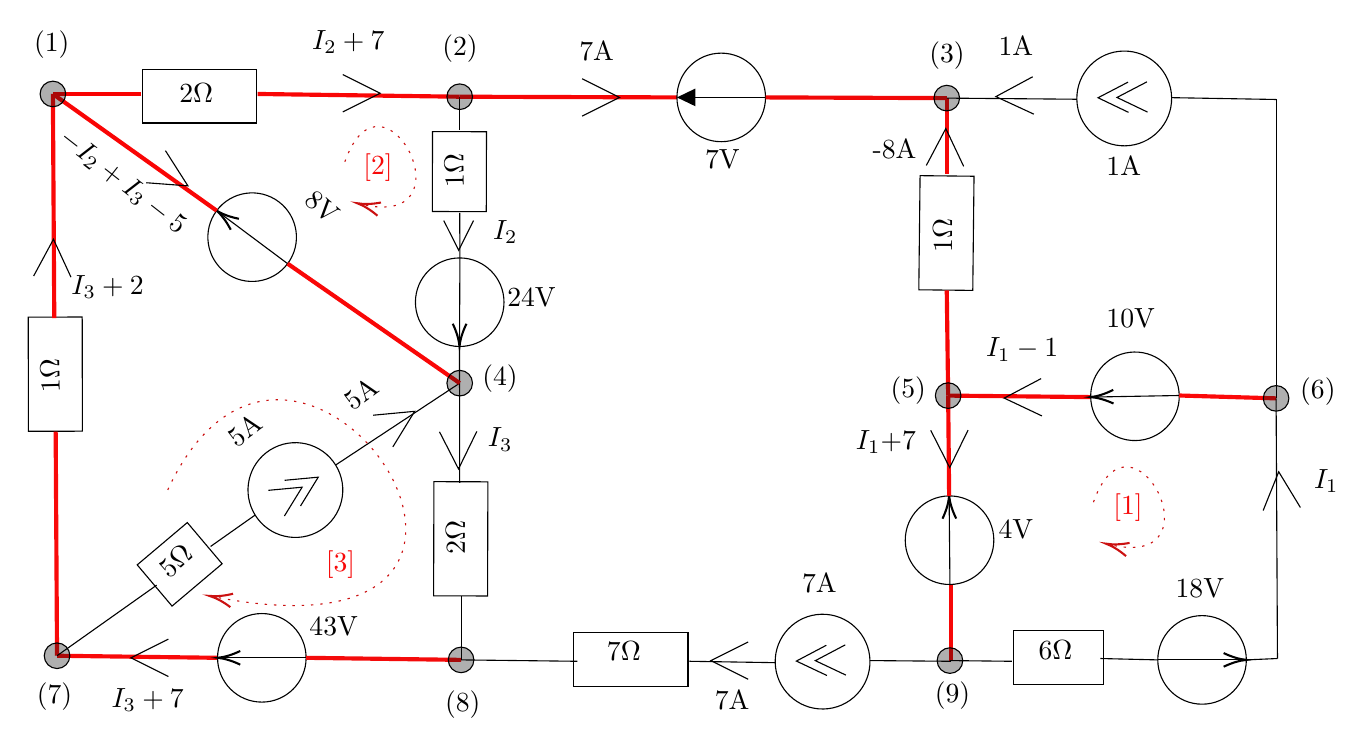
\begin{tikzpicture}[x=0.75pt,y=0.75pt,yscale=-1,xscale=1]
%uncomment if require: \path (0,398); %set diagram left start at 0, and has height of 398

%Flowchart: Connector [id:dp3845657900753279] 
\draw   (566.67,326.33) .. controls (566.67,314.55) and (576.22,305) .. (588,305) .. controls (599.78,305) and (609.33,314.55) .. (609.33,326.33) .. controls (609.33,338.12) and (599.78,347.67) .. (588,347.67) .. controls (576.22,347.67) and (566.67,338.12) .. (566.67,326.33) -- cycle ;
%Straight Lines [id:da16399958302066242] 
\draw    (566.67,326.33) -- (607.33,326.33) ;
\draw [shift={(609.33,326.33)}, rotate = 180] [color={rgb, 255:red, 0; green, 0; blue, 0 }  ][line width=0.75]    (10.93,-3.29) .. controls (6.95,-1.4) and (3.31,-0.3) .. (0,0) .. controls (3.31,0.3) and (6.95,1.4) .. (10.93,3.29)   ;

%Shape: Rectangle [id:dp2577955771553695] 
\draw   (497.33,312.33) -- (540.33,312.33) -- (540.33,338.33) -- (497.33,338.33) -- cycle ;
%Shape: Rectangle [id:dp5395909408827155] 
\draw   (77.33,41.67) -- (132.33,41.67) -- (132.33,67.67) -- (77.33,67.67) -- cycle ;
%Straight Lines [id:da9819662797927184] 
\draw [color={rgb, 255:red, 249; green, 2; blue, 2 }  ,draw opacity=1 ][line width=1.5]    (77,53.67) -- (34.33,53.67) ;
%Shape: Rectangle [id:dp2089139540837528] 
\draw   (48.45,161.14) -- (48.55,216.14) -- (22.55,216.19) -- (22.45,161.19) -- cycle ;
%Straight Lines [id:da9259746238050017] 
\draw [color={rgb, 255:red, 249; green, 7; blue, 7 }  ,draw opacity=1 ][line width=1.5]    (34.33,53.67) -- (35,161.67) ;
%Straight Lines [id:da6727499311363383] 
\draw [color={rgb, 255:red, 249; green, 10; blue, 10 }  ,draw opacity=1 ][line width=1.5]    (35.67,216.33) -- (36.33,324.33) ;
%Straight Lines [id:da05854884525038884] 
\draw [color={rgb, 255:red, 249; green, 9; blue, 9 }  ,draw opacity=1 ][line width=1.5]    (36.33,324.33) -- (113.67,325.33) ;
%Flowchart: Connector [id:dp8729559873962527] 
\draw   (156.33,325.33) .. controls (156.33,337.12) and (146.78,346.67) .. (135,346.67) .. controls (123.22,346.67) and (113.67,337.12) .. (113.67,325.33) .. controls (113.67,313.55) and (123.22,304) .. (135,304) .. controls (146.78,304) and (156.33,313.55) .. (156.33,325.33) -- cycle ;
%Straight Lines [id:da1974412985974312] 
\draw    (156.33,325.33) -- (115.67,325.33) ;
\draw [shift={(113.67,325.33)}, rotate = 360] [color={rgb, 255:red, 0; green, 0; blue, 0 }  ][line width=0.75]    (10.93,-3.29) .. controls (6.95,-1.4) and (3.31,-0.3) .. (0,0) .. controls (3.31,0.3) and (6.95,1.4) .. (10.93,3.29)   ;

%Straight Lines [id:da6163793132781621] 
\draw [color={rgb, 255:red, 244; green, 11; blue, 11 }  ,draw opacity=1 ][line width=1.5]    (231,326.33) -- (156.33,325.33) ;
%Straight Lines [id:da5155610054408897] 
\draw [color={rgb, 255:red, 249; green, 6; blue, 6 }  ,draw opacity=1 ][line width=1.5]    (133,53.67) -- (230.33,55) ;
%Straight Lines [id:da035475980090706516] 
\draw    (231,295.67) -- (231,326.33) ;
%Shape: Rectangle [id:dp9423684458314621] 
\draw   (243.91,240.54) -- (243.76,295.54) -- (217.76,295.46) -- (217.91,240.46) -- cycle ;
%Straight Lines [id:da30757280745923476] 
\draw    (230.33,55) -- (230.33,71) ;
%Shape: Rectangle [id:dp8494085552821424] 
\draw   (243.24,71.87) -- (243.14,110.38) -- (217.14,110.3) -- (217.24,71.8) -- cycle ;
%Straight Lines [id:da3959702190800809] 
\draw    (230.33,111) -- (230.44,132.67) ;
%Flowchart: Connector [id:dp8820531383018047] 
\draw   (230.44,132.67) .. controls (242.22,132.73) and (251.73,142.33) .. (251.67,154.11) .. controls (251.61,165.89) and (242.01,175.39) .. (230.23,175.33) .. controls (218.44,175.27) and (208.94,165.67) .. (209,153.89) .. controls (209.06,142.11) and (218.66,132.61) .. (230.44,132.67) -- cycle ;
%Straight Lines [id:da6746866455321117] 
\draw    (230.44,132.67) -- (230.24,173.33) ;
\draw [shift={(230.23,175.33)}, rotate = 270.29] [color={rgb, 255:red, 0; green, 0; blue, 0 }  ][line width=0.75]    (10.93,-3.29) .. controls (6.95,-1.4) and (3.31,-0.3) .. (0,0) .. controls (3.31,0.3) and (6.95,1.4) .. (10.93,3.29)   ;

%Straight Lines [id:da6116884732069012] 
\draw    (230.33,241) -- (230.23,175.33) ;
%Shape: Rectangle [id:dp1003407433166239] 
\draw   (74.96,280.55) -- (99.09,260.17) -- (115.87,280.03) -- (91.74,300.41) -- cycle ;
%Flowchart: Connector [id:dp14606866485045367] 
\draw   (131.77,256.55) .. controls (125.12,245.84) and (128.4,231.76) .. (139.11,225.11) .. controls (149.82,218.45) and (163.9,221.74) .. (170.56,232.45) .. controls (177.22,243.16) and (173.93,257.24) .. (163.22,263.89) .. controls (152.51,270.55) and (138.43,267.26) .. (131.77,256.55) -- cycle ;
\draw   (138.19,244.63) -- (154.41,243.13) -- (145.88,257) ;
\draw   (145.95,239.81) -- (162.17,238.3) -- (153.64,252.18) ;

%Straight Lines [id:da34840521409214276] 
\draw    (36.33,324.33) -- (84.33,290.33) ;
%Straight Lines [id:da8371724717521718] 
\draw    (131.77,256.55) -- (110.33,271.67) ;
%Straight Lines [id:da4891706641573459] 
\draw    (230.33,193) -- (170.56,232.45) ;
%Flowchart: Connector [id:dp6824147364869027] 
\draw   (147.43,135.43) .. controls (140.38,144.87) and (127.01,146.81) .. (117.57,139.76) .. controls (108.13,132.71) and (106.19,119.34) .. (113.24,109.9) .. controls (120.29,100.46) and (133.66,98.52) .. (143.1,105.57) .. controls (152.54,112.62) and (154.48,125.99) .. (147.43,135.43) -- cycle ;
%Straight Lines [id:da9205678856577881] 
\draw    (147.43,135.43) -- (114.84,111.1) ;
\draw [shift={(113.24,109.9)}, rotate = 36.75] [color={rgb, 255:red, 0; green, 0; blue, 0 }  ][line width=0.75]    (10.93,-3.29) .. controls (6.95,-1.4) and (3.31,-0.3) .. (0,0) .. controls (3.31,0.3) and (6.95,1.4) .. (10.93,3.29)   ;

%Straight Lines [id:da6919263546494281] 
\draw [color={rgb, 255:red, 249; green, 5; blue, 5 }  ,draw opacity=1 ][line width=1.5]    (34.33,53.67) -- (113.24,109.9) ;
%Straight Lines [id:da9806817330056354] 
\draw [color={rgb, 255:red, 249; green, 7; blue, 7 }  ,draw opacity=1 ][line width=1.5]    (147.43,135.43) -- (230.33,193) ;
%Straight Lines [id:da4293419307916777] 
\draw [color={rgb, 255:red, 247; green, 6; blue, 6 }  ,draw opacity=1 ][line width=1.5]    (230.33,55) -- (335,55.33) ;
%Flowchart: Connector [id:dp5905429133148798] 
\draw   (335,55.33) .. controls (335,43.55) and (344.55,34) .. (356.33,34) .. controls (368.12,34) and (377.67,43.55) .. (377.67,55.33) .. controls (377.67,67.12) and (368.12,76.67) .. (356.33,76.67) .. controls (344.55,76.67) and (335,67.12) .. (335,55.33) -- cycle ;
%Straight Lines [id:da9964888123159952] 
\draw    (338,55.33) -- (377.67,55.33) ;
\draw [shift={(335,55.33)}, rotate = 0] [fill={rgb, 255:red, 0; green, 0; blue, 0 }  ][line width=0.08]  [draw opacity=0] (8.93,-4.29) -- (0,0) -- (8.93,4.29) -- cycle    ;
%Straight Lines [id:da1898242648100037] 
\draw [color={rgb, 255:red, 241; green, 8; blue, 8 }  ,draw opacity=1 ][line width=1.5]    (377.67,55.33) -- (465,55.67) ;
%Straight Lines [id:da3294415007541591] 
\draw    (287,327) -- (231,326.33) ;
%Shape: Rectangle [id:dp11490755977265366] 
\draw   (285.33,313) -- (340.33,313) -- (340.33,339) -- (285.33,339) -- cycle ;
%Straight Lines [id:da6996779414528238] 
\draw    (382.34,327.67) -- (341,327) ;
%Flowchart: Connector [id:dp21779532152656977] 
\draw   (427.99,326.66) .. controls (428.27,339.27) and (418.28,349.72) .. (405.67,349.99) .. controls (393.06,350.27) and (382.62,340.28) .. (382.34,327.67) .. controls (382.06,315.06) and (392.06,304.62) .. (404.66,304.34) .. controls (417.27,304.06) and (427.72,314.06) .. (427.99,326.66) -- cycle ;
\draw   (416.4,333.66) -- (401.68,326.7) -- (416.08,319.1) ;
\draw   (407.27,333.86) -- (392.55,326.9) -- (406.95,319.3) ;

%Straight Lines [id:da9165720042883092] 
\draw    (467,327) -- (427.99,326.66) ;
%Straight Lines [id:da6769363901689145] 
\draw [color={rgb, 255:red, 247; green, 7; blue, 7 }  ,draw opacity=1 ][line width=1.5]    (467,290.33) -- (467,327) ;
%Flowchart: Connector [id:dp38679266638139387] 
\draw   (466.53,290) .. controls (454.75,290.11) and (445.11,280.65) .. (445,268.86) .. controls (444.89,257.08) and (454.35,247.44) .. (466.14,247.33) .. controls (477.92,247.23) and (487.56,256.69) .. (487.67,268.47) .. controls (487.77,280.25) and (478.31,289.89) .. (466.53,290) -- cycle ;
%Straight Lines [id:da7192186244884375] 
\draw    (466.53,290) -- (466.15,249.33) ;
\draw [shift={(466.14,247.33)}, rotate = 89.47] [color={rgb, 255:red, 0; green, 0; blue, 0 }  ][line width=0.75]    (10.93,-3.29) .. controls (6.95,-1.4) and (3.31,-0.3) .. (0,0) .. controls (3.31,0.3) and (6.95,1.4) .. (10.93,3.29)   ;

%Straight Lines [id:da8180476475710179] 
\draw [color={rgb, 255:red, 249; green, 6; blue, 6 }  ,draw opacity=1 ][line width=1.5]    (465.67,199) -- (466.14,247.33) ;
%Straight Lines [id:da0619442941070103] 
\draw [color={rgb, 255:red, 246; green, 7; blue, 7 }  ,draw opacity=1 ][line width=1.5]    (465,55.67) -- (465,92.33) ;
%Shape: Rectangle [id:dp8853596728704927] 
\draw   (478.13,93.31) -- (477.53,148.31) -- (451.53,148.02) -- (452.14,93.03) -- cycle ;
%Straight Lines [id:da7083644085402234] 
\draw [color={rgb, 255:red, 247; green, 6; blue, 6 }  ,draw opacity=1 ][line width=1.5]    (465.67,199) -- (465,148.33) ;
%Straight Lines [id:da19762246562272745] 
\draw    (465,55.67) -- (527.67,56.21) ;
%Flowchart: Connector [id:dp904294952747905] 
\draw   (573.33,55.45) .. controls (573.54,68.06) and (563.49,78.45) .. (550.88,78.66) .. controls (538.27,78.87) and (527.88,68.82) .. (527.67,56.21) .. controls (527.46,43.6) and (537.51,33.21) .. (550.12,33) .. controls (562.73,32.79) and (573.12,42.85) .. (573.33,55.45) -- cycle ;
\draw   (561.7,62.39) -- (547.01,55.35) -- (561.46,47.82) ;
\draw   (552.57,62.54) -- (537.88,55.5) -- (552.33,47.97) ;

%Straight Lines [id:da6046084287297446] 
\draw    (573.33,55.45) -- (623.67,56.33) ;
%Straight Lines [id:da5751838614974658] 
\draw    (623.67,56.33) -- (623.67,200.33) ;
%Straight Lines [id:da45774203391591994] 
\draw [color={rgb, 255:red, 247; green, 6; blue, 6 }  ,draw opacity=1 ][line width=1.5]    (534.34,199.72) -- (465.67,199) ;
%Flowchart: Connector [id:dp9690613790602691] 
\draw   (577,198.95) .. controls (577.21,210.73) and (567.83,220.45) .. (556.05,220.66) .. controls (544.27,220.88) and (534.55,211.5) .. (534.34,199.72) .. controls (534.12,187.94) and (543.5,178.22) .. (555.28,178) .. controls (567.06,177.79) and (576.78,187.17) .. (577,198.95) -- cycle ;
%Straight Lines [id:da2887844097342669] 
\draw    (577,198.95) -- (536.34,199.68) ;
\draw [shift={(534.34,199.72)}, rotate = 358.96] [color={rgb, 255:red, 0; green, 0; blue, 0 }  ][line width=0.75]    (10.93,-3.29) .. controls (6.95,-1.4) and (3.31,-0.3) .. (0,0) .. controls (3.31,0.3) and (6.95,1.4) .. (10.93,3.29)   ;

%Straight Lines [id:da4543189731044286] 
\draw [color={rgb, 255:red, 251; green, 9; blue, 9 }  ,draw opacity=1 ][line width=1.5]    (577,198.95) -- (623.67,200.33) ;
%Straight Lines [id:da08714308399957438] 
\draw    (466.53,326.67) -- (496.33,327) ;
%Straight Lines [id:da17382375080838308] 
\draw    (566.67,326.33) -- (539,325.67) ;
%Straight Lines [id:da17591417917014907] 
\draw    (623.67,200.33) -- (624.33,325.67) ;
%Straight Lines [id:da9491569937908073] 
\draw    (609.33,326.33) -- (624.33,325.67) ;
%Shape: Circle [id:dp39946719710190925] 
\draw  [fill={rgb, 255:red, 13; green, 12; blue, 12 }  ,fill opacity=0.33 ] (28.17,53.67) .. controls (28.17,50.26) and (30.93,47.5) .. (34.33,47.5) .. controls (37.74,47.5) and (40.5,50.26) .. (40.5,53.67) .. controls (40.5,57.07) and (37.74,59.83) .. (34.33,59.83) .. controls (30.93,59.83) and (28.17,57.07) .. (28.17,53.67) -- cycle ;
%Shape: Circle [id:dp21653719425053142] 
\draw  [fill={rgb, 255:red, 13; green, 12; blue, 12 }  ,fill opacity=0.33 ] (224.17,55) .. controls (224.17,51.59) and (226.93,48.83) .. (230.33,48.83) .. controls (233.74,48.83) and (236.5,51.59) .. (236.5,55) .. controls (236.5,58.41) and (233.74,61.17) .. (230.33,61.17) .. controls (226.93,61.17) and (224.17,58.41) .. (224.17,55) -- cycle ;
%Shape: Circle [id:dp24345331615652155] 
\draw  [fill={rgb, 255:red, 13; green, 12; blue, 12 }  ,fill opacity=0.33 ] (224.17,193) .. controls (224.17,189.59) and (226.93,186.83) .. (230.33,186.83) .. controls (233.74,186.83) and (236.5,189.59) .. (236.5,193) .. controls (236.5,196.41) and (233.74,199.17) .. (230.33,199.17) .. controls (226.93,199.17) and (224.17,196.41) .. (224.17,193) -- cycle ;
%Shape: Circle [id:dp16895975288384535] 
\draw  [fill={rgb, 255:red, 13; green, 12; blue, 12 }  ,fill opacity=0.33 ] (30.17,324.33) .. controls (30.17,320.93) and (32.93,318.17) .. (36.33,318.17) .. controls (39.74,318.17) and (42.5,320.93) .. (42.5,324.33) .. controls (42.5,327.74) and (39.74,330.5) .. (36.33,330.5) .. controls (32.93,330.5) and (30.17,327.74) .. (30.17,324.33) -- cycle ;
%Shape: Circle [id:dp598048275357975] 
\draw  [fill={rgb, 255:red, 13; green, 12; blue, 12 }  ,fill opacity=0.33 ] (224.83,326.33) .. controls (224.83,322.93) and (227.59,320.17) .. (231,320.17) .. controls (234.41,320.17) and (237.17,322.93) .. (237.17,326.33) .. controls (237.17,329.74) and (234.41,332.5) .. (231,332.5) .. controls (227.59,332.5) and (224.83,329.74) .. (224.83,326.33) -- cycle ;
%Shape: Circle [id:dp41622148120296654] 
\draw  [fill={rgb, 255:red, 13; green, 12; blue, 12 }  ,fill opacity=0.33 ] (458.83,55.67) .. controls (458.83,52.26) and (461.59,49.5) .. (465,49.5) .. controls (468.41,49.5) and (471.17,52.26) .. (471.17,55.67) .. controls (471.17,59.07) and (468.41,61.83) .. (465,61.83) .. controls (461.59,61.83) and (458.83,59.07) .. (458.83,55.67) -- cycle ;
%Shape: Circle [id:dp811559586012514] 
\draw  [fill={rgb, 255:red, 13; green, 12; blue, 12 }  ,fill opacity=0.33 ] (459.5,199) .. controls (459.5,195.59) and (462.26,192.83) .. (465.67,192.83) .. controls (469.07,192.83) and (471.83,195.59) .. (471.83,199) .. controls (471.83,202.41) and (469.07,205.17) .. (465.67,205.17) .. controls (462.26,205.17) and (459.5,202.41) .. (459.5,199) -- cycle ;
%Shape: Circle [id:dp2146664353696257] 
\draw  [fill={rgb, 255:red, 13; green, 12; blue, 12 }  ,fill opacity=0.33 ] (460.36,326.67) .. controls (460.36,323.26) and (463.12,320.5) .. (466.53,320.5) .. controls (469.94,320.5) and (472.7,323.26) .. (472.7,326.67) .. controls (472.7,330.07) and (469.94,332.83) .. (466.53,332.83) .. controls (463.12,332.83) and (460.36,330.07) .. (460.36,326.67) -- cycle ;
%Shape: Circle [id:dp6051563489559515] 
\draw  [fill={rgb, 255:red, 13; green, 12; blue, 12 }  ,fill opacity=0.33 ] (617.5,200.33) .. controls (617.5,196.93) and (620.26,194.17) .. (623.67,194.17) .. controls (627.07,194.17) and (629.83,196.93) .. (629.83,200.33) .. controls (629.83,203.74) and (627.07,206.5) .. (623.67,206.5) .. controls (620.26,206.5) and (617.5,203.74) .. (617.5,200.33) -- cycle ;
\draw   (174,44.33) -- (192,53.33) -- (174,62.33) ;
\draw   (88.56,80.99) -- (99.39,97.95) -- (79.32,96.44) ;
\draw   (25.06,141.38) -- (34.61,123.67) -- (43.05,141.94) ;
\draw   (90,334.33) -- (72,325.33) -- (90,316.33) ;
\draw   (188.6,208.45) -- (208.64,206.58) -- (198.11,223.73) ;
\draw   (238.58,216.25) -- (229.75,234.33) -- (220.59,216.42) ;
\draw   (237,114.65) -- (229.85,129) -- (222.66,114.68) ;
\draw   (369.33,335.67) -- (351.33,326.67) -- (369.33,317.67) ;
\draw   (289.33,46.33) -- (307.33,55.33) -- (289.33,64.33) ;
\draw   (455.14,88.13) -- (464.53,70.34) -- (473.13,88.53) ;
\draw   (506.94,63.39) -- (488.67,54.94) -- (506.39,45.39) ;
\draw   (510.86,208.8) -- (492.67,200.2) -- (510.47,190.8) ;
\draw   (475.27,215.6) -- (466.4,233.67) -- (457.27,215.73) ;
\draw   (617.43,254.37) -- (624.93,235.7) -- (635.37,252.9) ;
%Curve Lines [id:da8694221562471078] 
\draw [color={rgb, 255:red, 203; green, 17; blue, 17 }  ,draw opacity=1 ] [dash pattern={on 0.84pt off 2.51pt}]  (535.67,250.33) .. controls (554.15,198.19) and (598.11,283.92) .. (543.36,270.76) ;
\draw [shift={(541.67,270.33)}, rotate = 14.97] [color={rgb, 255:red, 203; green, 17; blue, 17 }  ,draw opacity=1 ][line width=0.75]    (10.93,-3.29) .. controls (6.95,-1.4) and (3.31,-0.3) .. (0,0) .. controls (3.31,0.3) and (6.95,1.4) .. (10.93,3.29)   ;

%Curve Lines [id:da6086378210342913] 
\draw [color={rgb, 255:red, 203; green, 17; blue, 17 }  ,draw opacity=1 ] [dash pattern={on 0.84pt off 2.51pt}]  (175,86.33) .. controls (193.48,34.19) and (237.44,119.92) .. (182.69,106.76) ;
\draw [shift={(181,106.33)}, rotate = 14.97] [color={rgb, 255:red, 203; green, 17; blue, 17 }  ,draw opacity=1 ][line width=0.75]    (10.93,-3.29) .. controls (6.95,-1.4) and (3.31,-0.3) .. (0,0) .. controls (3.31,0.3) and (6.95,1.4) .. (10.93,3.29)   ;

%Curve Lines [id:da4497642472341039] 
\draw [color={rgb, 255:red, 203; green, 17; blue, 17 }  ,draw opacity=1 ] [dash pattern={on 0.84pt off 2.51pt}]  (89.67,244.41) .. controls (152.18,109.86) and (301.78,334.67) .. (109.76,295.5) ;
\draw [shift={(109.76,295.5)}, rotate = 11.53] [color={rgb, 255:red, 203; green, 17; blue, 17 }  ,draw opacity=1 ][line width=0.75]    (10.93,-3.29) .. controls (6.95,-1.4) and (3.31,-0.3) .. (0,0) .. controls (3.31,0.3) and (6.95,1.4) .. (10.93,3.29)   ;


% Text Node
\draw (115.56,216.76) node [anchor=north west][inner sep=0.75pt]  [rotate=-322.88] [align=left] {5A};
% Text Node
\draw (156.67,304) node [anchor=north west][inner sep=0.75pt]   [align=left] {43V};
% Text Node
\draw (160.7,97.19) node [anchor=north west][inner sep=0.75pt]  [rotate=-41.03] [align=left] {8V};
% Text Node
\draw (252,145.67) node [anchor=north west][inner sep=0.75pt]   [align=left] {24V};
% Text Node
\draw (347.33,79) node [anchor=north west][inner sep=0.75pt]   [align=left] {7V};
% Text Node
\draw (394,283.67) node [anchor=north west][inner sep=0.75pt]   [align=left] {7A};
% Text Node
\draw (488.67,257.67) node [anchor=north west][inner sep=0.75pt]   [align=left] {4V};
% Text Node
\draw (574,285.67) node [anchor=north west][inner sep=0.75pt]   [align=left] {18V};
% Text Node
\draw (540.67,156) node [anchor=north west][inner sep=0.75pt]   [align=left] {10V};
% Text Node
\draw (540.67,82.67) node [anchor=north west][inner sep=0.75pt]   [align=left] {1A};
% Text Node
\draw (94,47.33) node [anchor=north west][inner sep=0.75pt]   [align=left] {2\ohm};
% Text Node
\draw (27.41,199.02) node [anchor=north west][inner sep=0.75pt]  [rotate=-268.74] [align=left] {1\ohm};
% Text Node
\draw (82.47,280.47) node [anchor=north west][inner sep=0.75pt]  [rotate=-318.32] [align=left] {5\ohm};
% Text Node
\draw (222.39,276.75) node [anchor=north west][inner sep=0.75pt]  [rotate=-270.58] [align=left] {2\ohm};
% Text Node
\draw (221.96,100.26) node [anchor=north west][inner sep=0.75pt]  [rotate=-269.34] [align=left] {1\ohm};
% Text Node
\draw (300,316.33) node [anchor=north west][inner sep=0.75pt]   [align=left] {7\ohm};
% Text Node
\draw (457.15,131.15) node [anchor=north west][inner sep=0.75pt]  [rotate=-270.09] [align=left] {1\ohm};
% Text Node
\draw (508,316) node [anchor=north west][inner sep=0.75pt]   [align=left] {6\ohm};
% Text Node
\draw (640.67,233.33) node [anchor=north west][inner sep=0.75pt]   [align=left] {$\displaystyle I_{1}$};
% Text Node
\draw (420,214.67) node [anchor=north west][inner sep=0.75pt]   [align=left] {$\displaystyle I_{1}$+7};
% Text Node
\draw (482.67,170) node [anchor=north west][inner sep=0.75pt]   [align=left] {$\displaystyle I_{1} -1$};
% Text Node
\draw (428,74.33) node [anchor=north west][inner sep=0.75pt]   [align=left] {\mbox{-}8A};
% Text Node
\draw (488.67,25) node [anchor=north west][inner sep=0.75pt]   [align=left] {1A};
% Text Node
\draw (286.67,27.33) node [anchor=north west][inner sep=0.75pt]   [align=left] {7A};
% Text Node
\draw (158,22) node [anchor=north west][inner sep=0.75pt]   [align=left] {$\displaystyle I_{2} +7$};
% Text Node
\draw (245.14,113.38) node [anchor=north west][inner sep=0.75pt]   [align=left] {$\displaystyle I_{2}$};
% Text Node
\draw (242.67,213.33) node [anchor=north west][inner sep=0.75pt]   [align=left] {$\displaystyle I_{3}$};
% Text Node
\draw (352,339.67) node [anchor=north west][inner sep=0.75pt]   [align=left] {7A};
% Text Node
\draw (61.33,338.67) node [anchor=north west][inner sep=0.75pt]   [align=left] {$\displaystyle I_{3} +7$};
% Text Node
\draw (171.57,199.27) node [anchor=north west][inner sep=0.75pt]  [rotate=-323.55] [align=left] {5A};
% Text Node
\draw (42,140) node [anchor=north west][inner sep=0.75pt]   [align=left] {$\displaystyle I_{3} +2$};
% Text Node
\draw (42.28,67.29) node [anchor=north west][inner sep=0.75pt]  [rotate=-38.09] [align=left] {$\displaystyle -I_{2} +I_{3} -5$};
% Text Node
\draw (544,245) node [anchor=north west][inner sep=0.75pt]  [color={rgb, 255:red, 247; green, 9; blue, 9 }  ,opacity=1 ] [align=left] {[1]};
% Text Node
\draw (182.67,81) node [anchor=north west][inner sep=0.75pt]  [color={rgb, 255:red, 247; green, 9; blue, 9 }  ,opacity=1 ] [align=left] {[2]};
% Text Node
\draw (164.56,272.66) node [anchor=north west][inner sep=0.75pt]  [color={rgb, 255:red, 247; green, 9; blue, 9 }  ,opacity=1 ] [align=left] {[3]};
% Text Node
\draw (24,22) node [anchor=north west][inner sep=0.75pt]   [align=left] {(1)};
% Text Node
\draw (220.67,24) node [anchor=north west][inner sep=0.75pt]   [align=left] {(2)};
% Text Node
\draw (455.33,27.33) node [anchor=north west][inner sep=0.75pt]   [align=left] {(3)};
% Text Node
\draw (240,183) node [anchor=north west][inner sep=0.75pt]   [align=left] {(4)};
% Text Node
\draw (436.67,188.67) node [anchor=north west][inner sep=0.75pt]   [align=left] {(5)};
% Text Node
\draw (634,189.33) node [anchor=north west][inner sep=0.75pt]   [align=left] {(6)};
% Text Node
\draw (25.33,336) node [anchor=north west][inner sep=0.75pt]   [align=left] {(7)};
% Text Node
\draw (222,340) node [anchor=north west][inner sep=0.75pt]   [align=left] {(8)};
% Text Node
\draw (458,335.67) node [anchor=north west][inner sep=0.75pt]   [align=left] {(9)};


\end{tikzpicture}

\end{center}
Rescriind ecuațiile rezultante din buclele [1], [2], [3] din \emph{Kirchhoff II} obținem următorul sistem:

\begin{equation}\nonumber
        \left\{
        \begin{array}{lr}
            -6I_1\;=\;-18 + 4 - 10\\[10pt]
            I_2 + 2(I_2 + 7)\;=\;24 + 8\\[10pt]
            2I_3 + (I_3 + 2) = 43 - 8
        \end{array}
        \right.
\end{equation}
Cum avem noroc acest sistem se rezolvă foarte ușor, rezultând soluția:
\begin{equation}\nonumber
        \left\{
        \begin{array}{lr}
            I_1\;=\;4A\\[10pt]
            I_2\;=\;6A\\[10pt]
            I_3\;=\;11A
        \end{array}
        \right.
\end{equation}
\newpage
\subsection{Graful de curenți, de tensiuni și bilanțul de puteri}
În urma rezolvărilor pașilor de mai sus am aflat toate intensitățile prezente în circuit.

\begin{center}
    

\tikzset{every picture/.style={line width=0.75pt}} %set default line width to 0.75pt        

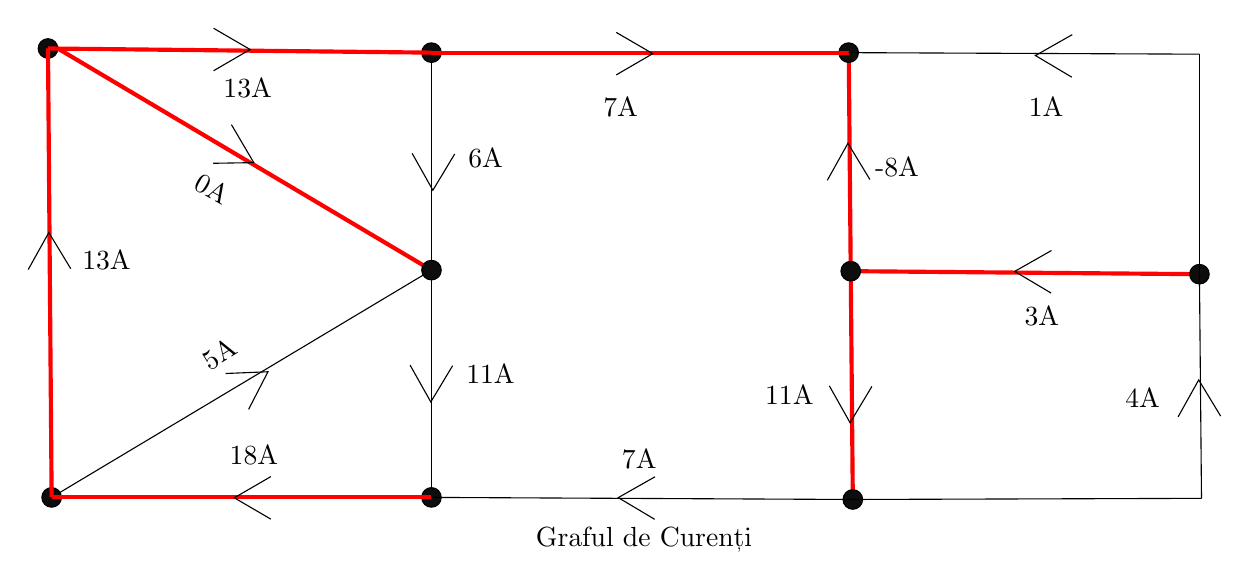
\begin{tikzpicture}[x=0.75pt,y=0.75pt,yscale=-1,xscale=1]
%uncomment if require: \path (0,300); %set diagram left start at 0, and has height of 300

%Straight Lines [id:da21045800549237814] 
\draw [color={rgb, 255:red, 251; green, 0; blue, 0 }  ,draw opacity=1 ][line width=1.5]    (443,266.05) -- (441,46.05) ;
%Straight Lines [id:da004890146660028849] 
\draw    (240,46.05) -- (240,265.05) ;
%Straight Lines [id:da9436228030524887] 
\draw [color={rgb, 255:red, 255; green, 0; blue, 0 }  ,draw opacity=1 ][line width=1.5]    (57,47) -- (240,155.55) ;
%Straight Lines [id:da5807636430233452] 
\draw    (57,265.05) -- (240,155.55) ;
%Straight Lines [id:da07520304550863566] 
\draw [color={rgb, 255:red, 251; green, 4; blue, 4 }  ,draw opacity=1 ][line width=1.5]    (610,157.5) -- (442,156.05) ;
%Shape: Circle [id:dp8908991627382346] 
\draw  [fill={rgb, 255:red, 14; green, 13; blue, 13 }  ,fill opacity=1 ] (50.52,48.76) .. controls (50.52,46.16) and (52.63,44.05) .. (55.24,44.05) .. controls (57.84,44.05) and (59.95,46.16) .. (59.95,48.76) .. controls (59.95,51.37) and (57.84,53.48) .. (55.24,53.48) .. controls (52.63,53.48) and (50.52,51.37) .. (50.52,48.76) -- cycle ;
%Shape: Circle [id:dp11473877397988663] 
\draw  [fill={rgb, 255:red, 14; green, 13; blue, 13 }  ,fill opacity=1 ] (52.29,265.05) .. controls (52.29,262.44) and (54.4,260.33) .. (57,260.33) .. controls (59.6,260.33) and (61.71,262.44) .. (61.71,265.05) .. controls (61.71,267.65) and (59.6,269.76) .. (57,269.76) .. controls (54.4,269.76) and (52.29,267.65) .. (52.29,265.05) -- cycle ;
%Shape: Circle [id:dp5807254321001776] 
\draw  [fill={rgb, 255:red, 14; green, 13; blue, 13 }  ,fill opacity=1 ] (235.29,155.55) .. controls (235.29,152.94) and (237.4,150.83) .. (240,150.83) .. controls (242.6,150.83) and (244.71,152.94) .. (244.71,155.55) .. controls (244.71,158.15) and (242.6,160.26) .. (240,160.26) .. controls (237.4,160.26) and (235.29,158.15) .. (235.29,155.55) -- cycle ;
%Shape: Circle [id:dp3646520570999061] 
\draw  [fill={rgb, 255:red, 14; green, 13; blue, 13 }  ,fill opacity=1 ] (235.29,50.76) .. controls (235.29,48.16) and (237.4,46.05) .. (240,46.05) .. controls (242.6,46.05) and (244.71,48.16) .. (244.71,50.76) .. controls (244.71,53.37) and (242.6,55.48) .. (240,55.48) .. controls (237.4,55.48) and (235.29,53.37) .. (235.29,50.76) -- cycle ;
%Shape: Circle [id:dp5825982820045075] 
\draw  [fill={rgb, 255:red, 14; green, 13; blue, 13 }  ,fill opacity=1 ] (235.29,265.05) .. controls (235.29,262.44) and (237.4,260.33) .. (240,260.33) .. controls (242.6,260.33) and (244.71,262.44) .. (244.71,265.05) .. controls (244.71,267.65) and (242.6,269.76) .. (240,269.76) .. controls (237.4,269.76) and (235.29,267.65) .. (235.29,265.05) -- cycle ;
%Shape: Circle [id:dp14863797103649068] 
\draw  [fill={rgb, 255:red, 14; green, 13; blue, 13 }  ,fill opacity=1 ] (437.29,156.05) .. controls (437.29,153.44) and (439.4,151.33) .. (442,151.33) .. controls (444.6,151.33) and (446.71,153.44) .. (446.71,156.05) .. controls (446.71,158.65) and (444.6,160.76) .. (442,160.76) .. controls (439.4,160.76) and (437.29,158.65) .. (437.29,156.05) -- cycle ;
%Shape: Circle [id:dp6624636049301356] 
\draw  [fill={rgb, 255:red, 14; green, 13; blue, 13 }  ,fill opacity=1 ] (436.29,50.76) .. controls (436.29,48.16) and (438.4,46.05) .. (441,46.05) .. controls (443.6,46.05) and (445.71,48.16) .. (445.71,50.76) .. controls (445.71,53.37) and (443.6,55.48) .. (441,55.48) .. controls (438.4,55.48) and (436.29,53.37) .. (436.29,50.76) -- cycle ;
%Shape: Circle [id:dp09770898595203037] 
\draw  [fill={rgb, 255:red, 14; green, 13; blue, 13 }  ,fill opacity=1 ] (438.29,266.05) .. controls (438.29,263.44) and (440.4,261.33) .. (443,261.33) .. controls (445.6,261.33) and (447.71,263.44) .. (447.71,266.05) .. controls (447.71,268.65) and (445.6,270.76) .. (443,270.76) .. controls (440.4,270.76) and (438.29,268.65) .. (438.29,266.05) -- cycle ;
%Shape: Circle [id:dp24800518053003495] 
\draw  [fill={rgb, 255:red, 14; green, 13; blue, 13 }  ,fill opacity=1 ] (605.29,157.5) .. controls (605.29,154.9) and (607.4,152.79) .. (610,152.79) .. controls (612.6,152.79) and (614.71,154.9) .. (614.71,157.5) .. controls (614.71,160.1) and (612.6,162.21) .. (610,162.21) .. controls (607.4,162.21) and (605.29,160.1) .. (605.29,157.5) -- cycle ;
%Straight Lines [id:da616679450964865] 
\draw [color={rgb, 255:red, 255; green, 0; blue, 0 }  ,draw opacity=1 ][line width=1.5]    (55.24,48.76) -- (240,50.76) ;
%Straight Lines [id:da45712321633467745] 
\draw [color={rgb, 255:red, 255; green, 0; blue, 0 }  ,draw opacity=1 ][fill={rgb, 255:red, 255; green, 0; blue, 0 }  ,fill opacity=1 ][line width=1.5]    (55.24,48.76) -- (57,265.05) ;
%Straight Lines [id:da7071492325225306] 
\draw [color={rgb, 255:red, 255; green, 0; blue, 0 }  ,draw opacity=1 ][line width=1.5]    (57,265.05) -- (240,265.05) ;
%Straight Lines [id:da5617837683084317] 
\draw [color={rgb, 255:red, 255; green, 0; blue, 0 }  ,draw opacity=1 ][line width=1.5]    (240,50.76) -- (441,50.76) ;
%Straight Lines [id:da7099031494228125] 
\draw    (443,266.05) -- (240,265.05) ;
%Straight Lines [id:da2756686295424895] 
\draw    (610,51.5) -- (441,50.76) ;
%Straight Lines [id:da9904378794079685] 
\draw    (610,51.5) -- (610,157.5) ;
%Straight Lines [id:da3335504328107153] 
\draw    (611,265.5) -- (443,266.05) ;
%Straight Lines [id:da3656330988117984] 
\draw    (611,265.5) -- (610,157.5) ;
\draw   (135,39) -- (152.62,49.25) -- (135,59.5) ;
\draw   (143.61,85.43) -- (154.38,103.75) -- (134.86,104.07) ;
\draw   (45.72,155.25) -- (55.65,137.44) -- (66.22,154.87) ;
\draw   (140.87,205.35) -- (161.23,204.51) -- (151.9,222.63) ;
\draw   (162.61,275.51) -- (145,265.24) -- (162.63,255.01) ;
\draw   (251.19,99.6) -- (240.68,117.06) -- (230.69,99.29) ;
\draw   (250.19,201.6) -- (239.68,219.06) -- (229.69,201.29) ;
\draw   (329,41) -- (346.62,51.25) -- (329,61.5) ;
\draw   (430.72,112.25) -- (440.65,94.44) -- (451.22,111.87) ;
\draw   (452.19,211.6) -- (441.68,229.06) -- (431.69,211.29) ;
\draw   (538.52,166.59) -- (521,156.16) -- (538.72,146.09) ;
\draw   (599.72,226.25) -- (609.65,208.44) -- (620.22,225.87) ;
\draw   (548.52,62.59) -- (531,52.16) -- (548.72,42.09) ;
\draw   (347.52,275.59) -- (330,265.16) -- (347.72,255.09) ;

% Text Node
\draw (157,67.75) node   [align=left] {\begin{minipage}[lt]{25.84pt}\setlength\topsep{0pt}
13A
\end{minipage}};
% Text Node
\draw (89,150.75) node   [align=left] {\begin{minipage}[lt]{25.84pt}\setlength\topsep{0pt}
13A
\end{minipage}};
% Text Node
\draw (145.29,191.22) node  [rotate=-328.16] [align=left] {\begin{minipage}[lt]{25.84pt}\setlength\topsep{0pt}
5A
\end{minipage}};
% Text Node
\draw (274,205.75) node   [align=left] {\begin{minipage}[lt]{25.84pt}\setlength\topsep{0pt}
11A
\end{minipage}};
% Text Node
\draw (160,244.75) node   [align=left] {\begin{minipage}[lt]{25.84pt}\setlength\topsep{0pt}
18A
\end{minipage}};
% Text Node
\draw (142,120.75) node  [rotate=-29.47] [align=left] {\begin{minipage}[lt]{25.84pt}\setlength\topsep{0pt}
0A
\end{minipage}};
% Text Node
\draw (275,101.75) node   [align=left] {\begin{minipage}[lt]{25.84pt}\setlength\topsep{0pt}
6A
\end{minipage}};
% Text Node
\draw (340,76.75) node   [align=left] {\begin{minipage}[lt]{25.84pt}\setlength\topsep{0pt}
7A
\end{minipage}};
% Text Node
\draw (545,76.75) node   [align=left] {\begin{minipage}[lt]{25.84pt}\setlength\topsep{0pt}
1A
\end{minipage}};
% Text Node
\draw (471,105.75) node   [align=left] {\begin{minipage}[lt]{25.84pt}\setlength\topsep{0pt}
\mbox{-}8A
\end{minipage}};
% Text Node
\draw (349,246.75) node   [align=left] {\begin{minipage}[lt]{25.84pt}\setlength\topsep{0pt}
7A
\end{minipage}};
% Text Node
\draw (418,215.75) node   [align=left] {\begin{minipage}[lt]{25.84pt}\setlength\topsep{0pt}
11A
\end{minipage}};
% Text Node
\draw (591.5,217.25) node   [align=left] {\begin{minipage}[lt]{25.84pt}\setlength\topsep{0pt}
4A
\end{minipage}};
% Text Node
\draw (543,177.75) node   [align=left] {\begin{minipage}[lt]{25.84pt}\setlength\topsep{0pt}
3A
\end{minipage}};
% Text Node
\draw (289,278) node [anchor=north west][inner sep=0.75pt]   [align=left] {Graful de Curenți};


\end{tikzpicture}

\end{center}

\begin{center}


\tikzset{every picture/.style={line width=0.75pt}} %set default line width to 0.75pt        

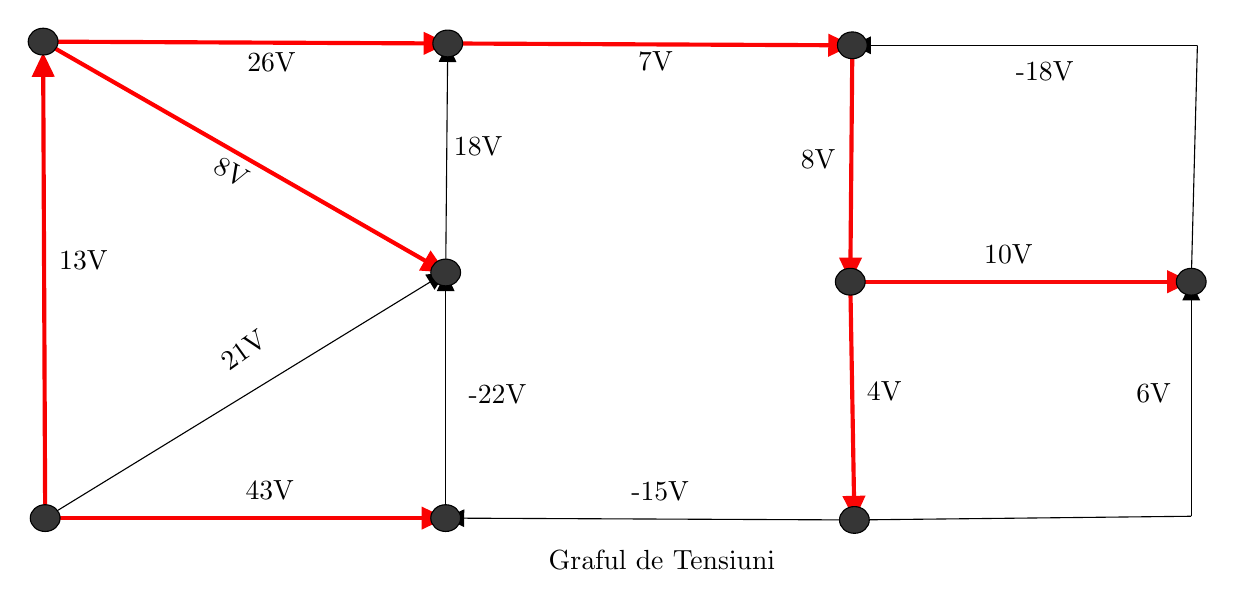
\begin{tikzpicture}[x=0.75pt,y=0.75pt,yscale=-1,xscale=1]
%uncomment if require: \path (0,300); %set diagram left start at 0, and has height of 300

%Straight Lines [id:da2007473758909839] 
\draw [color={rgb, 255:red, 254; green, 0; blue, 0 }  ,draw opacity=1 ][line width=1.5]    (44.01,19.28) -- (234.95,20.16) ;
\draw [shift={(238.95,20.17)}, rotate = 180.26] [fill={rgb, 255:red, 254; green, 0; blue, 0 }  ,fill opacity=1 ][line width=0.08]  [draw opacity=0] (11.61,-5.58) -- (0,0) -- (11.61,5.58) -- cycle    ;
%Straight Lines [id:da5805126599838257] 
\draw [color={rgb, 255:red, 247; green, 0; blue, 0 }  ,draw opacity=1 ][line width=1.5]    (45,248.85) -- (44.03,28.62) ;
\draw [shift={(44.01,24.62)}, rotate = 89.75] [fill={rgb, 255:red, 247; green, 0; blue, 0 }  ,fill opacity=1 ][line width=0.08]  [draw opacity=0] (11.61,-5.58) -- (0,0) -- (11.61,5.58) -- cycle    ;
%Straight Lines [id:da8738581165107147] 
\draw [color={rgb, 255:red, 249; green, 2; blue, 2 }  ,draw opacity=1 ][line width=1.5]    (45,248.85) -- (233.96,248.85) ;
\draw [shift={(237.96,248.85)}, rotate = 180] [fill={rgb, 255:red, 249; green, 2; blue, 2 }  ,fill opacity=1 ][line width=0.08]  [draw opacity=0] (11.61,-5.58) -- (0,0) -- (11.61,5.58) -- cycle    ;
%Straight Lines [id:da8246688638523951] 
\draw    (237.96,130.51) -- (238.92,23.17) ;
\draw [shift={(238.95,20.17)}, rotate = 90.51] [fill={rgb, 255:red, 0; green, 0; blue, 0 }  ][line width=0.08]  [draw opacity=0] (8.93,-4.29) -- (0,0) -- (8.93,4.29) -- cycle    ;
%Straight Lines [id:da1596653387550402] 
\draw    (237.96,248.85) -- (237.96,133.51) ;
\draw [shift={(237.96,130.51)}, rotate = 90] [fill={rgb, 255:red, 0; green, 0; blue, 0 }  ][line width=0.08]  [draw opacity=0] (8.93,-4.29) -- (0,0) -- (8.93,4.29) -- cycle    ;
%Straight Lines [id:da5555019763907534] 
\draw [color={rgb, 255:red, 255; green, 0; blue, 0 }  ,draw opacity=1 ][line width=1.5]    (44.01,19.28) -- (234.49,128.52) ;
\draw [shift={(237.96,130.51)}, rotate = 209.83] [fill={rgb, 255:red, 255; green, 0; blue, 0 }  ,fill opacity=1 ][line width=0.08]  [draw opacity=0] (11.61,-5.58) -- (0,0) -- (11.61,5.58) -- cycle    ;
%Straight Lines [id:da1584487637276637] 
\draw    (45,248.85) -- (235.4,132.08) ;
\draw [shift={(237.96,130.51)}, rotate = 148.48] [fill={rgb, 255:red, 0; green, 0; blue, 0 }  ][line width=0.08]  [draw opacity=0] (8.93,-4.29) -- (0,0) -- (8.93,4.29) -- cycle    ;
%Straight Lines [id:da07384074659043027] 
\draw [color={rgb, 255:red, 252; green, 4; blue, 4 }  ,draw opacity=1 ][line width=1.5]    (238.95,20.17) -- (429.89,21.05) ;
\draw [shift={(433.89,21.06)}, rotate = 180.26] [fill={rgb, 255:red, 252; green, 4; blue, 4 }  ,fill opacity=1 ][line width=0.08]  [draw opacity=0] (11.61,-5.58) -- (0,0) -- (11.61,5.58) -- cycle    ;
%Straight Lines [id:da6237409008125407] 
\draw    (434.87,249.74) -- (240.96,248.86) ;
\draw [shift={(237.96,248.85)}, rotate = 0.26] [fill={rgb, 255:red, 0; green, 0; blue, 0 }  ][line width=0.08]  [draw opacity=0] (8.93,-4.29) -- (0,0) -- (8.93,4.29) -- cycle    ;
%Straight Lines [id:da9464008767654883] 
\draw [color={rgb, 255:red, 247; green, 5; blue, 5 }  ,draw opacity=1 ][line width=1.5]    (433.89,21.06) -- (432.93,130.96) ;
\draw [shift={(432.9,134.96)}, rotate = 270.5] [fill={rgb, 255:red, 247; green, 5; blue, 5 }  ,fill opacity=1 ][line width=0.08]  [draw opacity=0] (11.61,-5.58) -- (0,0) -- (11.61,5.58) -- cycle    ;
%Straight Lines [id:da7590611938251033] 
\draw [color={rgb, 255:red, 251; green, 6; blue, 6 }  ,draw opacity=1 ][line width=1.5]    (432.9,134.96) -- (434.81,245.74) ;
\draw [shift={(434.87,249.74)}, rotate = 269.01] [fill={rgb, 255:red, 251; green, 6; blue, 6 }  ,fill opacity=1 ][line width=0.08]  [draw opacity=0] (11.61,-5.58) -- (0,0) -- (11.61,5.58) -- cycle    ;
%Straight Lines [id:da8684739282858722] 
\draw [color={rgb, 255:red, 249; green, 9; blue, 9 }  ,draw opacity=1 ][line width=1.5]    (432.9,134.96) -- (593.16,134.96) ;
\draw [shift={(597.16,134.96)}, rotate = 180] [fill={rgb, 255:red, 249; green, 9; blue, 9 }  ,fill opacity=1 ][line width=0.08]  [draw opacity=0] (11.61,-5.58) -- (0,0) -- (11.61,5.58) -- cycle    ;
%Straight Lines [id:da08465928321582727] 
\draw    (600.13,21.06) -- (436.89,21.06) ;
\draw [shift={(433.89,21.06)}, rotate = 360] [fill={rgb, 255:red, 0; green, 0; blue, 0 }  ][line width=0.08]  [draw opacity=0] (8.93,-4.29) -- (0,0) -- (8.93,4.29) -- cycle    ;
%Straight Lines [id:da07742523144624669] 
\draw    (600.13,21.06) -- (597.16,134.96) ;
%Straight Lines [id:da8674741768771632] 
\draw    (597.16,247.96) -- (597.16,137.96) ;
\draw [shift={(597.16,134.96)}, rotate = 90] [fill={rgb, 255:red, 0; green, 0; blue, 0 }  ][line width=0.08]  [draw opacity=0] (8.93,-4.29) -- (0,0) -- (8.93,4.29) -- cycle    ;
%Straight Lines [id:da3035074751642657] 
\draw    (434.87,249.74) -- (597.16,247.96) ;
%Shape: Ellipse [id:dp702105646651815] 
\draw  [fill={rgb, 255:red, 54; green, 54; blue, 54 }  ,fill opacity=1 ] (426.71,21.06) .. controls (426.71,17.5) and (429.92,14.61) .. (433.89,14.61) .. controls (437.85,14.61) and (441.06,17.5) .. (441.06,21.06) .. controls (441.06,24.63) and (437.85,27.51) .. (433.89,27.51) .. controls (429.92,27.51) and (426.71,24.63) .. (426.71,21.06) -- cycle ;
%Shape: Ellipse [id:dp20532633875874495] 
\draw  [fill={rgb, 255:red, 54; green, 54; blue, 54 }  ,fill opacity=1 ] (425.72,134.96) .. controls (425.72,131.39) and (428.93,128.51) .. (432.9,128.51) .. controls (436.86,128.51) and (440.07,131.39) .. (440.07,134.96) .. controls (440.07,138.52) and (436.86,141.41) .. (432.9,141.41) .. controls (428.93,141.41) and (425.72,138.52) .. (425.72,134.96) -- cycle ;
%Shape: Ellipse [id:dp7688627874216465] 
\draw  [fill={rgb, 255:red, 54; green, 54; blue, 54 }  ,fill opacity=1 ] (589.99,134.96) .. controls (589.99,131.39) and (593.2,128.51) .. (597.16,128.51) .. controls (601.12,128.51) and (604.33,131.39) .. (604.33,134.96) .. controls (604.33,138.52) and (601.12,141.41) .. (597.16,141.41) .. controls (593.2,141.41) and (589.99,138.52) .. (589.99,134.96) -- cycle ;
%Shape: Ellipse [id:dp4237078330938182] 
\draw  [fill={rgb, 255:red, 54; green, 54; blue, 54 }  ,fill opacity=1 ] (427.7,249.74) .. controls (427.7,246.18) and (430.91,243.29) .. (434.87,243.29) .. controls (438.84,243.29) and (442.05,246.18) .. (442.05,249.74) .. controls (442.05,253.3) and (438.84,256.19) .. (434.87,256.19) .. controls (430.91,256.19) and (427.7,253.3) .. (427.7,249.74) -- cycle ;
%Shape: Ellipse [id:dp9547436642438543] 
\draw  [fill={rgb, 255:red, 54; green, 54; blue, 54 }  ,fill opacity=1 ] (231.77,20.17) .. controls (231.77,16.61) and (234.98,13.72) .. (238.95,13.72) .. controls (242.91,13.72) and (246.12,16.61) .. (246.12,20.17) .. controls (246.12,23.74) and (242.91,26.63) .. (238.95,26.63) .. controls (234.98,26.63) and (231.77,23.74) .. (231.77,20.17) -- cycle ;
%Shape: Ellipse [id:dp7949325370928308] 
\draw  [fill={rgb, 255:red, 54; green, 54; blue, 54 }  ,fill opacity=1 ] (230.78,130.51) .. controls (230.78,126.95) and (233.99,124.06) .. (237.96,124.06) .. controls (241.92,124.06) and (245.13,126.95) .. (245.13,130.51) .. controls (245.13,134.07) and (241.92,136.96) .. (237.96,136.96) .. controls (233.99,136.96) and (230.78,134.07) .. (230.78,130.51) -- cycle ;
%Shape: Ellipse [id:dp44539204376449804] 
\draw  [fill={rgb, 255:red, 54; green, 54; blue, 54 }  ,fill opacity=1 ] (230.78,248.85) .. controls (230.78,245.29) and (233.99,242.4) .. (237.96,242.4) .. controls (241.92,242.4) and (245.13,245.29) .. (245.13,248.85) .. controls (245.13,252.41) and (241.92,255.3) .. (237.96,255.3) .. controls (233.99,255.3) and (230.78,252.41) .. (230.78,248.85) -- cycle ;
%Shape: Ellipse [id:dp21768997242867516] 
\draw  [fill={rgb, 255:red, 54; green, 54; blue, 54 }  ,fill opacity=1 ] (37.82,248.85) .. controls (37.82,245.29) and (41.03,242.4) .. (45,242.4) .. controls (48.96,242.4) and (52.17,245.29) .. (52.17,248.85) .. controls (52.17,252.41) and (48.96,255.3) .. (45,255.3) .. controls (41.03,255.3) and (37.82,252.41) .. (37.82,248.85) -- cycle ;
%Shape: Ellipse [id:dp5490196740132514] 
\draw  [fill={rgb, 255:red, 54; green, 54; blue, 54 }  ,fill opacity=1 ] (36.83,19.28) .. controls (36.83,15.72) and (40.05,12.83) .. (44.01,12.83) .. controls (47.97,12.83) and (51.18,15.72) .. (51.18,19.28) .. controls (51.18,22.85) and (47.97,25.74) .. (44.01,25.74) .. controls (40.05,25.74) and (36.83,22.85) .. (36.83,19.28) -- cycle ;

% Text Node
\draw (141.1,23.42) node [anchor=north west][inner sep=0.75pt]   [align=left] {26V};
% Text Node
\draw (50.49,118.47) node [anchor=north west][inner sep=0.75pt]   [align=left] {13V};
% Text Node
\draw (129.35,72.04) node [anchor=north west][inner sep=0.75pt]  [rotate=-29.97] [align=left] {8V};
% Text Node
\draw (126.61,170.68) node [anchor=north west][inner sep=0.75pt]  [rotate=-324.47] [align=left] {21V};
% Text Node
\draw (140.28,229.66) node [anchor=north west][inner sep=0.75pt]   [align=left] {43V};
% Text Node
\draw (247.77,183.42) node [anchor=north west][inner sep=0.75pt]   [align=left] {\mbox{-}22V};
% Text Node
\draw (240.68,63.79) node [anchor=north west][inner sep=0.75pt]   [align=left] {18V};
% Text Node
\draw (329.46,23.05) node [anchor=north west][inner sep=0.75pt]   [align=left] {7V};
% Text Node
\draw (326.13,230.03) node [anchor=north west][inner sep=0.75pt]   [align=left] {\mbox{-}15V};
% Text Node
\draw (439.65,181.59) node [anchor=north west][inner sep=0.75pt]   [align=left] {4V};
% Text Node
\draw (569.44,182.69) node [anchor=north west][inner sep=0.75pt]   [align=left] {6V};
% Text Node
\draw (407.82,70.02) node [anchor=north west][inner sep=0.75pt]   [align=left] {8V};
% Text Node
\draw (511.42,27.82) node [anchor=north west][inner sep=0.75pt]   [align=left] {\mbox{-}18V};
% Text Node
\draw (496.17,115.9) node [anchor=north west][inner sep=0.75pt]   [align=left] {10V};
% Text Node
\draw (286.33,263.06) node [anchor=north west][inner sep=0.75pt]   [align=left] {Graful de Tensiuni};


\end{tikzpicture}

\end{center}
Acum că am aflat cele două grafuri și avem și circuitul electric rezistiv liniar complet, vom verifica bilanțul de puteri ($P_c = P_g$).
$$P_c = 1\cdot13^2 + 2\cdot13^2 + 5\cdot5^2 + 1\cdot6^2 + 2\cdot11^2 + 7\cdot7^2 + 1\cdot8^2 + 6\cdot4^2 = 1413W$$
$$P_g = -8\cdot0 - 7\cdot7 +24\cdot6 + 10\cdot3 + 43\cdot18 - 4\cdot11 + 18\cdot4 + 4\cdot5 + 64\cdot7 + 18\cdot1 = 1413W$$

\newpage

\section{Generatorul echivalent de tensiune}
În această secțiune vom transforma circuitul electric liniar rezistiv din secțiunile de mai sus într-un generator echivalent de tensiune, față de bornele (1) și (2):

\begin{center}
    

\tikzset{every picture/.style={line width=0.75pt}} %set default line width to 0.75pt        

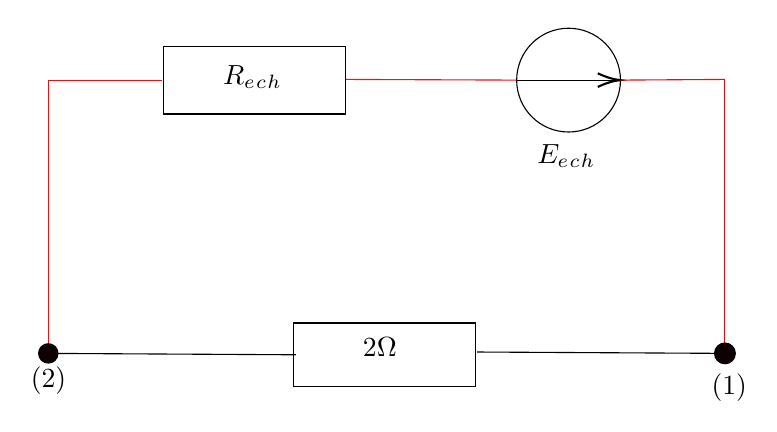
\begin{tikzpicture}[x=0.75pt,y=0.75pt,yscale=-1,xscale=1]
%uncomment if require: \path (0,300); %set diagram left start at 0, and has height of 300

%Straight Lines [id:da3224313797429348] 
\draw    (362.33,191.67) -- (481.67,192.33) ;
%Shape: Rectangle [id:dp6893354233123505] 
\draw   (273.67,177.67) -- (361.67,177.67) -- (361.67,208.33) -- (273.67,208.33) -- cycle ;
%Straight Lines [id:da9223439565409108] 
\draw    (155.67,192.33) -- (275,193) ;
%Straight Lines [id:da4026004964078189] 
\draw [color={rgb, 255:red, 249; green, 12; blue, 12 }  ,draw opacity=1 ]   (155.67,61) -- (155.67,192.33) ;
%Straight Lines [id:da7755220774610179] 
\draw [color={rgb, 255:red, 242; green, 8; blue, 8 }  ,draw opacity=1 ]   (481.67,60.33) -- (481.67,192.33) ;
%Shape: Rectangle [id:dp5308903226746371] 
\draw   (211,44.33) -- (299,44.33) -- (299,77) -- (211,77) -- cycle ;
%Shape: Circle [id:dp513529319607058] 
\draw   (381.33,60.67) .. controls (381.33,46.86) and (392.53,35.67) .. (406.33,35.67) .. controls (420.14,35.67) and (431.33,46.86) .. (431.33,60.67) .. controls (431.33,74.47) and (420.14,85.67) .. (406.33,85.67) .. controls (392.53,85.67) and (381.33,74.47) .. (381.33,60.67) -- cycle ;
%Straight Lines [id:da6344708178258509] 
\draw    (381.33,60.67) -- (429.33,60.67) ;
\draw [shift={(431.33,60.67)}, rotate = 180] [color={rgb, 255:red, 0; green, 0; blue, 0 }  ][line width=0.75]    (10.93,-3.29) .. controls (6.95,-1.4) and (3.31,-0.3) .. (0,0) .. controls (3.31,0.3) and (6.95,1.4) .. (10.93,3.29)   ;

%Straight Lines [id:da5413569904406206] 
\draw [color={rgb, 255:red, 247; green, 10; blue, 10 }  ,draw opacity=1 ]   (210.33,61) -- (155.67,61) ;
%Straight Lines [id:da9673200830998514] 
\draw [color={rgb, 255:red, 241; green, 18; blue, 18 }  ,draw opacity=1 ]   (299,60.33) -- (381.33,60.67) ;
%Straight Lines [id:da9317028525661359] 
\draw [color={rgb, 255:red, 244; green, 9; blue, 9 }  ,draw opacity=1 ]   (481.67,60.33) -- (431.33,60.67) ;
%Shape: Circle [id:dp19423452087766102] 
\draw  [fill={rgb, 255:red, 13; green, 1; blue, 1 }  ,fill opacity=1 ] (476.67,192.33) .. controls (476.67,189.57) and (478.91,187.33) .. (481.67,187.33) .. controls (484.43,187.33) and (486.67,189.57) .. (486.67,192.33) .. controls (486.67,195.09) and (484.43,197.33) .. (481.67,197.33) .. controls (478.91,197.33) and (476.67,195.09) .. (476.67,192.33) -- cycle ;
%Shape: Circle [id:dp6097035217414721] 
\draw  [fill={rgb, 255:red, 13; green, 1; blue, 1 }  ,fill opacity=1 ] (151,192.33) .. controls (151,189.76) and (153.09,187.67) .. (155.67,187.67) .. controls (158.24,187.67) and (160.33,189.76) .. (160.33,192.33) .. controls (160.33,194.91) and (158.24,197) .. (155.67,197) .. controls (153.09,197) and (151,194.91) .. (151,192.33) -- cycle ;

% Text Node
\draw (474,201) node [anchor=north west][inner sep=0.75pt]   [align=left] {(1)};
% Text Node
\draw (146,197.33) node [anchor=north west][inner sep=0.75pt]   [align=left] {(2)};
% Text Node
\draw (306,183.67) node [anchor=north west][inner sep=0.75pt]   [align=left] {$\displaystyle 2\si{\ohm}$};
% Text Node
\draw (238.67,52.33) node [anchor=north west][inner sep=0.75pt]   [align=left] {$\displaystyle R_{e}{}_{c}{}_{h}$};
% Text Node
\draw (390,90.33) node [anchor=north west][inner sep=0.75pt]   [align=left] {$\displaystyle E_{e}{}_{c}{}_{h}$};


\end{tikzpicture}

\end{center}
Din teorema lui \emph{Thevenin} rezultă că $E_{ech} = U_{120}$ și $R_{ech} = R_{120}|pasivizat$.\\
Pentru a putea afla în primul rând tensiunea echivalentă ne vom folosi de unealta dedicată \emph{LTSpice}, unde vom tăia din circuit rezistorul dintre bornele (1) și (2) și vom plasa nodul de masă la nodul (2), apoi V(1) va fi $E_{ech}$.
\subsection{Determinarea tensiunii și rezistenței de mers în gol}

\begin{center}
    

\tikzset{every picture/.style={line width=0.75pt}} %set default line width to 0.75pt        

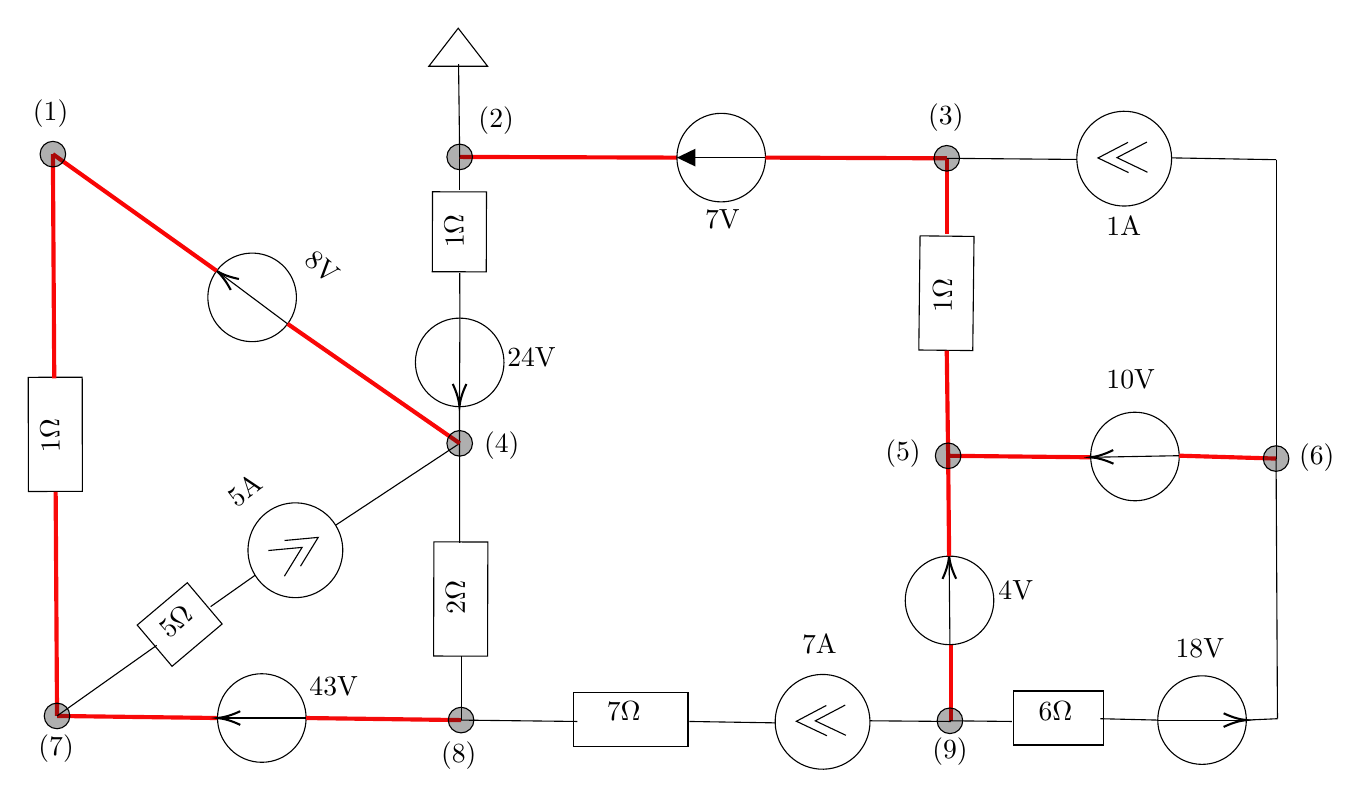
\begin{tikzpicture}[x=0.75pt,y=0.75pt,yscale=-1,xscale=1]
%uncomment if require: \path (0,441); %set diagram left start at 0, and has height of 441

%Flowchart: Connector [id:dp9270801755221227] 
\draw   (589.21,364.67) .. controls (589.21,352.88) and (598.76,343.33) .. (610.54,343.33) .. controls (622.33,343.33) and (631.88,352.88) .. (631.88,364.67) .. controls (631.88,376.45) and (622.33,386) .. (610.54,386) .. controls (598.76,386) and (589.21,376.45) .. (589.21,364.67) -- cycle ;
%Straight Lines [id:da6781562055832304] 
\draw    (589.21,364.67) -- (629.88,364.67) ;
\draw [shift={(631.88,364.67)}, rotate = 180] [color={rgb, 255:red, 0; green, 0; blue, 0 }  ][line width=0.75]    (10.93,-3.29) .. controls (6.95,-1.4) and (3.31,-0.3) .. (0,0) .. controls (3.31,0.3) and (6.95,1.4) .. (10.93,3.29)   ;

%Shape: Rectangle [id:dp4737566977396117] 
\draw   (519.88,350.67) -- (562.88,350.67) -- (562.88,376.67) -- (519.88,376.67) -- cycle ;
%Shape: Rectangle [id:dp9667802879586256] 
\draw   (71,199.48) -- (71.09,254.48) -- (45.09,254.52) -- (45,199.52) -- cycle ;
%Straight Lines [id:da7347210402357076] 
\draw [color={rgb, 255:red, 249; green, 7; blue, 7 }  ,draw opacity=1 ][line width=1.5]    (56.88,92) -- (57.54,200) ;
%Straight Lines [id:da30746269499196677] 
\draw [color={rgb, 255:red, 249; green, 10; blue, 10 }  ,draw opacity=1 ][line width=1.5]    (58.21,254.67) -- (58.88,362.67) ;
%Straight Lines [id:da16528068153435105] 
\draw [color={rgb, 255:red, 249; green, 9; blue, 9 }  ,draw opacity=1 ][line width=1.5]    (58.88,362.67) -- (136.21,363.67) ;
%Flowchart: Connector [id:dp40061918108006433] 
\draw   (178.88,363.67) .. controls (178.88,375.45) and (169.33,385) .. (157.54,385) .. controls (145.76,385) and (136.21,375.45) .. (136.21,363.67) .. controls (136.21,351.88) and (145.76,342.33) .. (157.54,342.33) .. controls (169.33,342.33) and (178.88,351.88) .. (178.88,363.67) -- cycle ;
%Straight Lines [id:da4449167399874583] 
\draw    (178.88,363.67) -- (138.21,363.67) ;
\draw [shift={(136.21,363.67)}, rotate = 360] [color={rgb, 255:red, 0; green, 0; blue, 0 }  ][line width=0.75]    (10.93,-3.29) .. controls (6.95,-1.4) and (3.31,-0.3) .. (0,0) .. controls (3.31,0.3) and (6.95,1.4) .. (10.93,3.29)   ;

%Straight Lines [id:da5423321266401198] 
\draw [color={rgb, 255:red, 244; green, 11; blue, 11 }  ,draw opacity=1 ][line width=1.5]    (253.54,364.67) -- (178.88,363.67) ;
%Straight Lines [id:da6672889723585598] 
\draw    (253.54,334) -- (253.54,364.67) ;
%Shape: Rectangle [id:dp2916318610646307] 
\draw   (266.45,278.87) -- (266.3,333.87) -- (240.3,333.8) -- (240.45,278.8) -- cycle ;
%Straight Lines [id:da1333229254706947] 
\draw    (252.88,93.33) -- (252.88,109.33) ;
%Shape: Rectangle [id:dp8147511147447091] 
\draw   (265.79,110.2) -- (265.68,148.71) -- (239.68,148.64) -- (239.79,110.13) -- cycle ;
%Straight Lines [id:da3752772298769764] 
\draw    (252.88,149.33) -- (252.99,171) ;
%Flowchart: Connector [id:dp9800044826411813] 
\draw   (252.99,171) .. controls (264.77,171.06) and (274.27,180.66) .. (274.21,192.44) .. controls (274.15,204.22) and (264.55,213.73) .. (252.77,213.67) .. controls (240.99,213.61) and (231.49,204.01) .. (231.54,192.23) .. controls (231.6,180.44) and (241.2,170.94) .. (252.99,171) -- cycle ;
%Straight Lines [id:da15518000296251477] 
\draw    (252.99,171) -- (252.78,211.67) ;
\draw [shift={(252.77,213.67)}, rotate = 270.29] [color={rgb, 255:red, 0; green, 0; blue, 0 }  ][line width=0.75]    (10.93,-3.29) .. controls (6.95,-1.4) and (3.31,-0.3) .. (0,0) .. controls (3.31,0.3) and (6.95,1.4) .. (10.93,3.29)   ;

%Straight Lines [id:da5102374999677335] 
\draw    (252.88,279.33) -- (252.77,213.67) ;
%Shape: Rectangle [id:dp4139885664271359] 
\draw   (97.51,318.88) -- (121.64,298.5) -- (138.42,318.36) -- (114.29,338.75) -- cycle ;
%Flowchart: Connector [id:dp8841244253872094] 
\draw   (154.32,294.89) .. controls (147.66,284.18) and (150.95,270.1) .. (161.66,263.44) .. controls (172.37,256.78) and (186.45,260.07) .. (193.1,270.78) .. controls (199.76,281.49) and (196.47,295.57) .. (185.76,302.23) .. controls (175.05,308.88) and (160.97,305.6) .. (154.32,294.89) -- cycle ;
\draw   (160.73,282.96) -- (176.95,281.46) -- (168.42,295.34) ;
\draw   (168.49,278.14) -- (184.71,276.64) -- (176.18,290.52) ;

%Straight Lines [id:da6498485089903523] 
\draw    (58.88,362.67) -- (106.88,328.67) ;
%Straight Lines [id:da1648330757903893] 
\draw    (154.32,294.89) -- (132.88,310) ;
%Straight Lines [id:da25570294871250665] 
\draw    (252.88,231.33) -- (193.1,270.78) ;
%Flowchart: Connector [id:dp5578065010047788] 
\draw   (169.97,173.76) .. controls (162.92,183.2) and (149.55,185.14) .. (140.11,178.09) .. controls (130.67,171.04) and (128.74,157.68) .. (135.78,148.24) .. controls (142.83,138.8) and (156.2,136.86) .. (165.64,143.91) .. controls (175.08,150.96) and (177.02,164.32) .. (169.97,173.76) -- cycle ;
%Straight Lines [id:da23421547181746738] 
\draw    (169.97,173.76) -- (137.39,149.43) ;
\draw [shift={(135.78,148.24)}, rotate = 36.75] [color={rgb, 255:red, 0; green, 0; blue, 0 }  ][line width=0.75]    (10.93,-3.29) .. controls (6.95,-1.4) and (3.31,-0.3) .. (0,0) .. controls (3.31,0.3) and (6.95,1.4) .. (10.93,3.29)   ;

%Straight Lines [id:da3360778513474214] 
\draw [color={rgb, 255:red, 249; green, 5; blue, 5 }  ,draw opacity=1 ][line width=1.5]    (56.88,92) -- (135.78,148.24) ;
%Straight Lines [id:da1355482709182445] 
\draw [color={rgb, 255:red, 249; green, 7; blue, 7 }  ,draw opacity=1 ][line width=1.5]    (169.97,173.76) -- (252.88,231.33) ;
%Straight Lines [id:da10802524495699561] 
\draw [color={rgb, 255:red, 247; green, 6; blue, 6 }  ,draw opacity=1 ][line width=1.5]    (252.88,93.33) -- (357.54,93.67) ;
%Flowchart: Connector [id:dp5057766104260943] 
\draw   (357.54,93.67) .. controls (357.54,81.88) and (367.1,72.33) .. (378.88,72.33) .. controls (390.66,72.33) and (400.21,81.88) .. (400.21,93.67) .. controls (400.21,105.45) and (390.66,115) .. (378.88,115) .. controls (367.1,115) and (357.54,105.45) .. (357.54,93.67) -- cycle ;
%Straight Lines [id:da3181224817766224] 
\draw    (360.54,93.67) -- (400.21,93.67) ;
\draw [shift={(357.54,93.67)}, rotate = 0] [fill={rgb, 255:red, 0; green, 0; blue, 0 }  ][line width=0.08]  [draw opacity=0] (8.93,-4.29) -- (0,0) -- (8.93,4.29) -- cycle    ;
%Straight Lines [id:da5180293715512814] 
\draw [color={rgb, 255:red, 241; green, 8; blue, 8 }  ,draw opacity=1 ][line width=1.5]    (400.21,93.67) -- (487.54,94) ;
%Straight Lines [id:da6785576903938952] 
\draw    (309.54,365.33) -- (253.54,364.67) ;
%Shape: Rectangle [id:dp43490317766124353] 
\draw   (307.88,351.33) -- (362.88,351.33) -- (362.88,377.33) -- (307.88,377.33) -- cycle ;
%Straight Lines [id:da06229672444698431] 
\draw    (404.88,366) -- (363.54,365.33) ;
%Flowchart: Connector [id:dp7851498713964808] 
\draw   (450.54,365) .. controls (450.82,377.61) and (440.82,388.05) .. (428.21,388.33) .. controls (415.61,388.61) and (405.16,378.61) .. (404.88,366) .. controls (404.61,353.39) and (414.6,342.95) .. (427.21,342.67) .. controls (439.82,342.39) and (450.26,352.39) .. (450.54,365) -- cycle ;
\draw   (438.95,372) -- (424.22,365.03) -- (438.63,357.43) ;
\draw   (429.82,372.2) -- (415.09,365.23) -- (429.5,357.63) ;

%Straight Lines [id:da9185246580674729] 
\draw    (489.54,365.33) -- (450.54,365) ;
%Straight Lines [id:da750326464081535] 
\draw [color={rgb, 255:red, 247; green, 7; blue, 7 }  ,draw opacity=1 ][line width=1.5]    (489.54,328.67) -- (489.54,365.33) ;
%Flowchart: Connector [id:dp2681269475222585] 
\draw   (489.08,328.33) .. controls (477.29,328.44) and (467.65,318.98) .. (467.55,307.2) .. controls (467.44,295.42) and (476.9,285.78) .. (488.68,285.67) .. controls (500.46,285.56) and (510.1,295.02) .. (510.21,306.8) .. controls (510.32,318.58) and (500.86,328.22) .. (489.08,328.33) -- cycle ;
%Straight Lines [id:da46089558980747936] 
\draw    (489.08,328.33) -- (488.7,287.67) ;
\draw [shift={(488.68,285.67)}, rotate = 89.47] [color={rgb, 255:red, 0; green, 0; blue, 0 }  ][line width=0.75]    (10.93,-3.29) .. controls (6.95,-1.4) and (3.31,-0.3) .. (0,0) .. controls (3.31,0.3) and (6.95,1.4) .. (10.93,3.29)   ;

%Straight Lines [id:da2321409034543207] 
\draw [color={rgb, 255:red, 249; green, 6; blue, 6 }  ,draw opacity=1 ][line width=1.5]    (488.21,237.33) -- (488.68,285.67) ;
%Straight Lines [id:da8769965982394923] 
\draw [color={rgb, 255:red, 246; green, 7; blue, 7 }  ,draw opacity=1 ][line width=1.5]    (487.54,94) -- (487.54,130.67) ;
%Shape: Rectangle [id:dp4867788140885223] 
\draw   (500.68,131.64) -- (500.07,186.64) -- (474.08,186.36) -- (474.68,131.36) -- cycle ;
%Straight Lines [id:da7875812451856252] 
\draw [color={rgb, 255:red, 247; green, 6; blue, 6 }  ,draw opacity=1 ][line width=1.5]    (488.21,237.33) -- (487.54,186.67) ;
%Straight Lines [id:da6536587562096758] 
\draw    (487.54,94) -- (550.21,94.55) ;
%Flowchart: Connector [id:dp17553917091137916] 
\draw   (595.87,93.79) .. controls (596.08,106.4) and (586.03,116.79) .. (573.42,117) .. controls (560.81,117.21) and (550.42,107.15) .. (550.21,94.55) .. controls (550.01,81.94) and (560.06,71.55) .. (572.67,71.34) .. controls (585.27,71.13) and (595.67,81.18) .. (595.87,93.79) -- cycle ;
\draw   (584.25,100.72) -- (569.56,93.68) -- (584,86.16) ;
\draw   (575.11,100.87) -- (560.42,93.83) -- (574.87,86.31) ;

%Straight Lines [id:da18482728121268854] 
\draw    (595.87,93.79) -- (646.21,94.67) ;
%Straight Lines [id:da7498258113423346] 
\draw    (646.21,94.67) -- (646.21,238.67) ;
%Straight Lines [id:da940259620577877] 
\draw [color={rgb, 255:red, 247; green, 6; blue, 6 }  ,draw opacity=1 ][line width=1.5]    (556.88,238.05) -- (488.21,237.33) ;
%Flowchart: Connector [id:dp6624088763704992] 
\draw   (599.54,237.28) .. controls (599.76,249.06) and (590.38,258.78) .. (578.6,259) .. controls (566.82,259.21) and (557.1,249.83) .. (556.88,238.05) .. controls (556.67,226.27) and (566.04,216.55) .. (577.82,216.34) .. controls (589.6,216.12) and (599.33,225.5) .. (599.54,237.28) -- cycle ;
%Straight Lines [id:da5732322951082511] 
\draw    (599.54,237.28) -- (558.88,238.02) ;
\draw [shift={(556.88,238.05)}, rotate = 358.96] [color={rgb, 255:red, 0; green, 0; blue, 0 }  ][line width=0.75]    (10.93,-3.29) .. controls (6.95,-1.4) and (3.31,-0.3) .. (0,0) .. controls (3.31,0.3) and (6.95,1.4) .. (10.93,3.29)   ;

%Straight Lines [id:da7773054828023371] 
\draw [color={rgb, 255:red, 251; green, 9; blue, 9 }  ,draw opacity=1 ][line width=1.5]    (599.54,237.28) -- (646.21,238.67) ;
%Straight Lines [id:da9651126430027448] 
\draw    (489.08,365) -- (518.88,365.33) ;
%Straight Lines [id:da23967528935399973] 
\draw    (589.21,364.67) -- (561.54,364) ;
%Straight Lines [id:da9296553319859571] 
\draw    (646.21,238.67) -- (646.88,364) ;
%Straight Lines [id:da38754316585407866] 
\draw    (631.88,364.67) -- (646.88,364) ;
%Shape: Circle [id:dp7882674071011084] 
\draw  [fill={rgb, 255:red, 13; green, 12; blue, 12 }  ,fill opacity=0.33 ] (50.71,92) .. controls (50.71,88.59) and (53.47,85.83) .. (56.88,85.83) .. controls (60.28,85.83) and (63.04,88.59) .. (63.04,92) .. controls (63.04,95.41) and (60.28,98.17) .. (56.88,98.17) .. controls (53.47,98.17) and (50.71,95.41) .. (50.71,92) -- cycle ;
%Shape: Circle [id:dp7538292901722516] 
\draw  [fill={rgb, 255:red, 13; green, 12; blue, 12 }  ,fill opacity=0.33 ] (246.71,93.33) .. controls (246.71,89.93) and (249.47,87.17) .. (252.88,87.17) .. controls (256.28,87.17) and (259.04,89.93) .. (259.04,93.33) .. controls (259.04,96.74) and (256.28,99.5) .. (252.88,99.5) .. controls (249.47,99.5) and (246.71,96.74) .. (246.71,93.33) -- cycle ;
%Shape: Circle [id:dp24657752652752118] 
\draw  [fill={rgb, 255:red, 13; green, 12; blue, 12 }  ,fill opacity=0.33 ] (246.71,231.33) .. controls (246.71,227.93) and (249.47,225.17) .. (252.88,225.17) .. controls (256.28,225.17) and (259.04,227.93) .. (259.04,231.33) .. controls (259.04,234.74) and (256.28,237.5) .. (252.88,237.5) .. controls (249.47,237.5) and (246.71,234.74) .. (246.71,231.33) -- cycle ;
%Shape: Circle [id:dp8023182388888381] 
\draw  [fill={rgb, 255:red, 13; green, 12; blue, 12 }  ,fill opacity=0.33 ] (52.71,362.67) .. controls (52.71,359.26) and (55.47,356.5) .. (58.88,356.5) .. controls (62.28,356.5) and (65.04,359.26) .. (65.04,362.67) .. controls (65.04,366.07) and (62.28,368.83) .. (58.88,368.83) .. controls (55.47,368.83) and (52.71,366.07) .. (52.71,362.67) -- cycle ;
%Shape: Circle [id:dp9965555730253974] 
\draw  [fill={rgb, 255:red, 13; green, 12; blue, 12 }  ,fill opacity=0.33 ] (247.38,364.67) .. controls (247.38,361.26) and (250.14,358.5) .. (253.54,358.5) .. controls (256.95,358.5) and (259.71,361.26) .. (259.71,364.67) .. controls (259.71,368.07) and (256.95,370.83) .. (253.54,370.83) .. controls (250.14,370.83) and (247.38,368.07) .. (247.38,364.67) -- cycle ;
%Shape: Circle [id:dp4863208895647082] 
\draw  [fill={rgb, 255:red, 13; green, 12; blue, 12 }  ,fill opacity=0.33 ] (481.38,94) .. controls (481.38,90.59) and (484.14,87.83) .. (487.54,87.83) .. controls (490.95,87.83) and (493.71,90.59) .. (493.71,94) .. controls (493.71,97.41) and (490.95,100.17) .. (487.54,100.17) .. controls (484.14,100.17) and (481.38,97.41) .. (481.38,94) -- cycle ;
%Shape: Circle [id:dp14045591679570468] 
\draw  [fill={rgb, 255:red, 13; green, 12; blue, 12 }  ,fill opacity=0.33 ] (482.04,237.33) .. controls (482.04,233.93) and (484.81,231.17) .. (488.21,231.17) .. controls (491.62,231.17) and (494.38,233.93) .. (494.38,237.33) .. controls (494.38,240.74) and (491.62,243.5) .. (488.21,243.5) .. controls (484.81,243.5) and (482.04,240.74) .. (482.04,237.33) -- cycle ;
%Shape: Circle [id:dp15823477089237037] 
\draw  [fill={rgb, 255:red, 13; green, 12; blue, 12 }  ,fill opacity=0.33 ] (482.91,365) .. controls (482.91,361.59) and (485.67,358.83) .. (489.08,358.83) .. controls (492.48,358.83) and (495.24,361.59) .. (495.24,365) .. controls (495.24,368.4) and (492.48,371.17) .. (489.08,371.17) .. controls (485.67,371.17) and (482.91,368.4) .. (482.91,365) -- cycle ;
%Shape: Circle [id:dp677101212612778] 
\draw  [fill={rgb, 255:red, 13; green, 12; blue, 12 }  ,fill opacity=0.33 ] (640.04,238.67) .. controls (640.04,235.26) and (642.81,232.5) .. (646.21,232.5) .. controls (649.62,232.5) and (652.38,235.26) .. (652.38,238.67) .. controls (652.38,242.07) and (649.62,244.83) .. (646.21,244.83) .. controls (642.81,244.83) and (640.04,242.07) .. (640.04,238.67) -- cycle ;
%Straight Lines [id:da3213476677310445] 
\draw    (252.33,48.67) -- (252.88,93.33) ;
%Shape: Triangle [id:dp7531206299066631] 
\draw   (252.17,31.33) -- (266.33,49.67) -- (238,49.67) -- cycle ;

% Text Node
\draw (138.11,255.09) node [anchor=north west][inner sep=0.75pt]  [rotate=-322.88] [align=left] {5A};
% Text Node
\draw (179.21,342.33) node [anchor=north west][inner sep=0.75pt]   [align=left] {43V};
% Text Node
\draw (183.25,135.52) node [anchor=north west][inner sep=0.75pt]  [rotate=-41.03] [align=left] {8V};
% Text Node
\draw (274.54,184) node [anchor=north west][inner sep=0.75pt]   [align=left] {24V};
% Text Node
\draw (369.88,117.33) node [anchor=north west][inner sep=0.75pt]   [align=left] {7V};
% Text Node
\draw (416.54,322) node [anchor=north west][inner sep=0.75pt]   [align=left] {7A};
% Text Node
\draw (511.21,296) node [anchor=north west][inner sep=0.75pt]   [align=left] {4V};
% Text Node
\draw (596.54,324) node [anchor=north west][inner sep=0.75pt]   [align=left] {18V};
% Text Node
\draw (563.21,194.33) node [anchor=north west][inner sep=0.75pt]   [align=left] {10V};
% Text Node
\draw (563.21,121) node [anchor=north west][inner sep=0.75pt]   [align=left] {1A};
% Text Node
\draw (49.96,237.35) node [anchor=north west][inner sep=0.75pt]  [rotate=-268.74] [align=left] {1\ohm};
% Text Node
\draw (105.01,318.8) node [anchor=north west][inner sep=0.75pt]  [rotate=-318.32] [align=left] {5\ohm};
% Text Node
\draw (244.93,315.08) node [anchor=north west][inner sep=0.75pt]  [rotate=-270.58] [align=left] {2\ohm};
% Text Node
\draw (244.51,138.6) node [anchor=north west][inner sep=0.75pt]  [rotate=-269.34] [align=left] {1\ohm};
% Text Node
\draw (322.54,354.67) node [anchor=north west][inner sep=0.75pt]   [align=left] {7\ohm};
% Text Node
\draw (479.69,169.49) node [anchor=north west][inner sep=0.75pt]  [rotate=-270.09] [align=left] {1\ohm};
% Text Node
\draw (530.54,354.33) node [anchor=north west][inner sep=0.75pt]   [align=left] {6\ohm};
% Text Node
\draw (46,64.33) node [anchor=north west][inner sep=0.75pt]   [align=left] {(1)};
% Text Node
\draw (260.67,68) node [anchor=north west][inner sep=0.75pt]   [align=left] {(2)};
% Text Node
\draw (477.33,66.33) node [anchor=north west][inner sep=0.75pt]   [align=left] {(3)};
% Text Node
\draw (263.33,224.33) node [anchor=north west][inner sep=0.75pt]   [align=left] {(4)};
% Text Node
\draw (456.67,228.33) node [anchor=north west][inner sep=0.75pt]   [align=left] {(5)};
% Text Node
\draw (656,230.33) node [anchor=north west][inner sep=0.75pt]   [align=left] {(6)};
% Text Node
\draw (48.67,370.33) node [anchor=north west][inner sep=0.75pt]   [align=left] {(7)};
% Text Node
\draw (242.67,374) node [anchor=north west][inner sep=0.75pt]   [align=left] {(8)};
% Text Node
\draw (479.33,372) node [anchor=north west][inner sep=0.75pt]   [align=left] {(9)};


\end{tikzpicture}

\end{center}
\newpage
Rulând acest circuit în \emph{LTSpice} obținem următoarea valoare pentru potențialul nodului (1), care va fi și tensiunea electromotoare căutată:
\begin{figure}[h]
    \centering
    \includegraphics[width=\linewidth, height=\textheight, keepaspectratio]{Tensiune_echivalenta.png}
    \caption{Tensiunea echivalentă}
    \label{fig:euler}
\end{figure}

Pentru a putea obține rezistența echivalentă, vom scurtcicuita circuitul echivalent, prin plasarea unui \textbf{SIT} cu valoarea \textbf{0}, între bornele (1) și (2), cum tensiunea echivalentă este pozitivă rezultă că intensitatea de scurtcircuit este orientată de la borna (1) la borna (2).

\begin{center}
    

\tikzset{every picture/.style={line width=0.75pt}} %set default line width to 0.75pt        

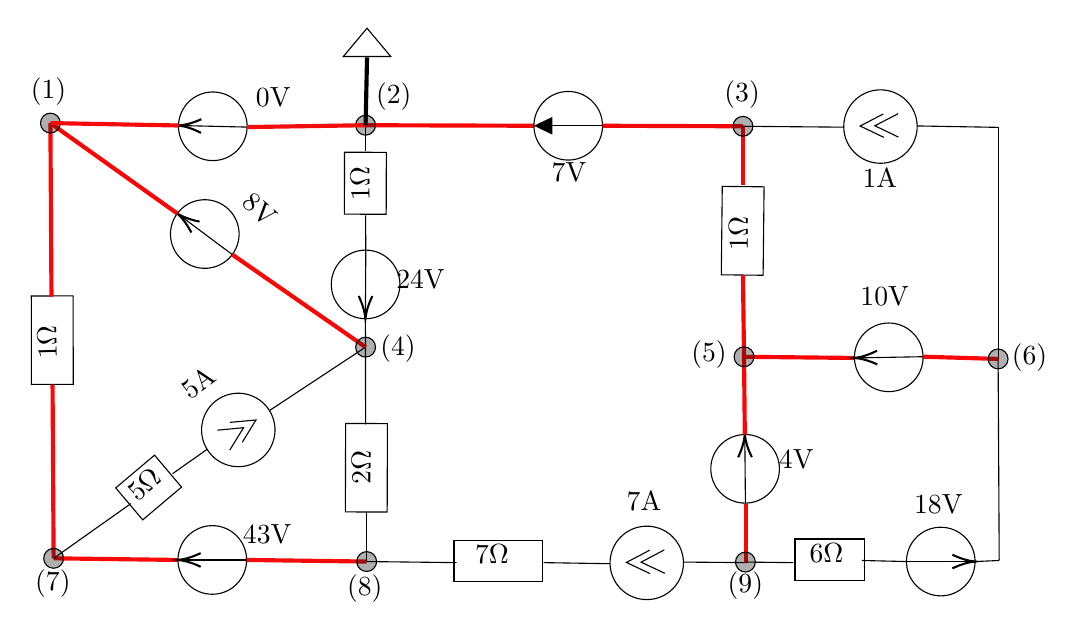
\begin{tikzpicture}[x=0.75pt,y=0.75pt,yscale=-1,xscale=1]
%uncomment if require: \path (0,441); %set diagram left start at 0, and has height of 441

%Flowchart: Connector [id:dp9270801755221227] 
\draw   (466.49,293.45) .. controls (466.49,284.32) and (473.89,276.92) .. (483.02,276.92) .. controls (492.14,276.92) and (499.54,284.32) .. (499.54,293.45) .. controls (499.54,302.58) and (492.14,309.98) .. (483.02,309.98) .. controls (473.89,309.98) and (466.49,302.58) .. (466.49,293.45) -- cycle ;
%Straight Lines [id:da6781562055832304] 
\draw    (466.49,293.45) -- (497.54,293.45) ;
\draw [shift={(499.54,293.45)}, rotate = 180] [color={rgb, 255:red, 0; green, 0; blue, 0 }  ][line width=0.75]    (10.93,-3.29) .. controls (6.95,-1.4) and (3.31,-0.3) .. (0,0) .. controls (3.31,0.3) and (6.95,1.4) .. (10.93,3.29)   ;

%Shape: Rectangle [id:dp4737566977396117] 
\draw   (412.77,282.61) -- (446.08,282.61) -- (446.08,302.75) -- (412.77,302.75) -- cycle ;
%Shape: Rectangle [id:dp9667802879586256] 
\draw   (64.98,165.47) -- (65.06,208.08) -- (44.91,208.11) -- (44.84,165.5) -- cycle ;
%Straight Lines [id:da7347210402357076] 
\draw [color={rgb, 255:red, 249; green, 7; blue, 7 }  ,draw opacity=1 ][line width=1.5]    (54.04,82.2) -- (54.56,165.87) ;
%Straight Lines [id:da30746269499196677] 
\draw [color={rgb, 255:red, 249; green, 10; blue, 10 }  ,draw opacity=1 ][line width=1.5]    (55.08,208.23) -- (55.59,291.9) ;
%Straight Lines [id:da16528068153435105] 
\draw [color={rgb, 255:red, 249; green, 9; blue, 9 }  ,draw opacity=1 ][line width=1.5]    (55.59,291.9) -- (115.51,292.68) ;
%Flowchart: Connector [id:dp40061918108006433] 
\draw   (148.57,292.68) .. controls (148.57,301.81) and (141.17,309.21) .. (132.04,309.21) .. controls (122.91,309.21) and (115.51,301.81) .. (115.51,292.68) .. controls (115.51,283.55) and (122.91,276.15) .. (132.04,276.15) .. controls (141.17,276.15) and (148.57,283.55) .. (148.57,292.68) -- cycle ;
%Straight Lines [id:da4449167399874583] 
\draw    (148.57,292.68) -- (117.51,292.68) ;
\draw [shift={(115.51,292.68)}, rotate = 360] [color={rgb, 255:red, 0; green, 0; blue, 0 }  ][line width=0.75]    (10.93,-3.29) .. controls (6.95,-1.4) and (3.31,-0.3) .. (0,0) .. controls (3.31,0.3) and (6.95,1.4) .. (10.93,3.29)   ;

%Straight Lines [id:da5423321266401198] 
\draw [color={rgb, 255:red, 244; green, 11; blue, 11 }  ,draw opacity=1 ][line width=1.5]    (206.42,293.45) -- (148.57,292.68) ;
%Straight Lines [id:da6672889723585598] 
\draw    (206.42,269.69) -- (206.42,293.45) ;
%Shape: Rectangle [id:dp2916318610646307] 
\draw   (216.42,226.98) -- (216.3,269.59) -- (196.16,269.54) -- (196.28,226.92) -- cycle ;
%Straight Lines [id:da1333229254706947] 
\draw    (205.9,83.23) -- (205.9,95.62) ;
%Shape: Rectangle [id:dp8147511147447091] 
\draw   (215.9,96.3) -- (215.82,126.13) -- (195.68,126.08) -- (195.76,96.24) -- cycle ;
%Straight Lines [id:da3752772298769764] 
\draw    (205.9,126.62) -- (205.99,143.4) ;
%Flowchart: Connector [id:dp9800044826411813] 
\draw   (205.99,143.4) .. controls (215.11,143.45) and (222.48,150.89) .. (222.43,160.02) .. controls (222.38,169.14) and (214.95,176.51) .. (205.82,176.46) .. controls (196.69,176.41) and (189.33,168.98) .. (189.37,159.85) .. controls (189.42,150.72) and (196.86,143.36) .. (205.99,143.4) -- cycle ;
%Straight Lines [id:da15518000296251477] 
\draw    (205.99,143.4) -- (205.83,174.46) ;
\draw [shift={(205.82,176.46)}, rotate = 270.29] [color={rgb, 255:red, 0; green, 0; blue, 0 }  ][line width=0.75]    (10.93,-3.29) .. controls (6.95,-1.4) and (3.31,-0.3) .. (0,0) .. controls (3.31,0.3) and (6.95,1.4) .. (10.93,3.29)   ;

%Straight Lines [id:da5102374999677335] 
\draw    (205.9,227.34) -- (205.82,176.46) ;
%Shape: Rectangle [id:dp4139885664271359] 
\draw   (85.52,257.98) -- (104.22,242.19) -- (117.22,257.58) -- (98.52,273.37) -- cycle ;
%Flowchart: Connector [id:dp8841244253872094] 
\draw   (129.54,239.39) .. controls (124.38,231.09) and (126.93,220.18) .. (135.23,215.02) .. controls (143.53,209.87) and (154.43,212.41) .. (159.59,220.71) .. controls (164.75,229.01) and (162.2,239.92) .. (153.9,245.08) .. controls (145.6,250.23) and (134.7,247.69) .. (129.54,239.39) -- cycle ;
\draw   (134.51,230.15) -- (147.08,228.98) -- (140.47,239.74) ;
\draw   (140.52,226.41) -- (153.09,225.25) -- (146.48,236) ;

%Straight Lines [id:da6498485089903523] 
\draw    (55.59,291.9) -- (92.78,265.56) ;
%Straight Lines [id:da1648330757903893] 
\draw    (129.54,239.39) -- (112.93,251.1) ;
%Straight Lines [id:da25570294871250665] 
\draw    (205.9,190.15) -- (159.59,220.71) ;
%Flowchart: Connector [id:dp5578065010047788] 
\draw   (141.67,145.54) .. controls (136.21,152.86) and (125.85,154.36) .. (118.53,148.9) .. controls (111.22,143.44) and (109.72,133.08) .. (115.18,125.77) .. controls (120.64,118.45) and (131,116.95) .. (138.31,122.41) .. controls (145.63,127.87) and (147.13,138.23) .. (141.67,145.54) -- cycle ;
%Straight Lines [id:da23421547181746738] 
\draw    (141.67,145.54) -- (116.78,126.96) ;
\draw [shift={(115.18,125.77)}, rotate = 36.75] [color={rgb, 255:red, 0; green, 0; blue, 0 }  ][line width=0.75]    (10.93,-3.29) .. controls (6.95,-1.4) and (3.31,-0.3) .. (0,0) .. controls (3.31,0.3) and (6.95,1.4) .. (10.93,3.29)   ;

%Straight Lines [id:da3360778513474214] 
\draw [color={rgb, 255:red, 249; green, 5; blue, 5 }  ,draw opacity=1 ][line width=1.5]    (54.04,82.2) -- (115.18,125.77) ;
%Straight Lines [id:da1355482709182445] 
\draw [color={rgb, 255:red, 249; green, 7; blue, 7 }  ,draw opacity=1 ][line width=1.5]    (141.67,145.54) -- (205.9,190.15) ;
%Straight Lines [id:da10802524495699561] 
\draw [color={rgb, 255:red, 247; green, 6; blue, 6 }  ,draw opacity=1 ][line width=1.5]    (205.9,83.23) -- (287,83.49) ;
%Flowchart: Connector [id:dp5057766104260943] 
\draw   (287,83.49) .. controls (287,74.36) and (294.4,66.96) .. (303.52,66.96) .. controls (312.65,66.96) and (320.05,74.36) .. (320.05,83.49) .. controls (320.05,92.62) and (312.65,100.02) .. (303.52,100.02) .. controls (294.4,100.02) and (287,92.62) .. (287,83.49) -- cycle ;
%Straight Lines [id:da3181224817766224] 
\draw    (290,83.49) -- (320.05,83.49) ;
\draw [shift={(287,83.49)}, rotate = 0] [fill={rgb, 255:red, 0; green, 0; blue, 0 }  ][line width=0.08]  [draw opacity=0] (8.93,-4.29) -- (0,0) -- (8.93,4.29) -- cycle    ;
%Straight Lines [id:da5180293715512814] 
\draw [color={rgb, 255:red, 241; green, 8; blue, 8 }  ,draw opacity=1 ][line width=1.5]    (320.05,83.49) -- (387.72,83.74) ;
%Straight Lines [id:da6785576903938952] 
\draw    (249.81,293.97) -- (206.42,293.45) ;
%Shape: Rectangle [id:dp43490317766124353] 
\draw   (248.51,283.12) -- (291.13,283.12) -- (291.13,303.27) -- (248.51,303.27) -- cycle ;
%Straight Lines [id:da06229672444698431] 
\draw    (323.67,294.49) -- (291.64,293.97) ;
%Flowchart: Connector [id:dp7851498713964808] 
\draw   (359.05,293.71) .. controls (359.26,303.48) and (351.52,311.57) .. (341.75,311.78) .. controls (331.98,312) and (323.89,304.26) .. (323.67,294.49) .. controls (323.46,284.72) and (331.2,276.63) .. (340.97,276.41) .. controls (350.74,276.2) and (358.83,283.94) .. (359.05,293.71) -- cycle ;
\draw   (350.06,299.13) -- (338.66,293.74) -- (349.82,287.85) ;
\draw   (342.99,299.29) -- (331.58,293.89) -- (342.74,288) ;

%Straight Lines [id:da9185246580674729] 
\draw    (389.27,293.97) -- (359.05,293.71) ;
%Straight Lines [id:da750326464081535] 
\draw [color={rgb, 255:red, 247; green, 7; blue, 7 }  ,draw opacity=1 ][line width=1.5]    (389.27,265.56) -- (389.27,293.97) ;
%Flowchart: Connector [id:dp2681269475222585] 
\draw   (388.9,265.3) .. controls (379.77,265.39) and (372.31,258.05) .. (372.22,248.93) .. controls (372.14,239.8) and (379.47,232.33) .. (388.6,232.25) .. controls (397.73,232.16) and (405.19,239.49) .. (405.28,248.62) .. controls (405.36,257.75) and (398.03,265.22) .. (388.9,265.3) -- cycle ;
%Straight Lines [id:da46089558980747936] 
\draw    (388.9,265.3) -- (388.62,234.25) ;
\draw [shift={(388.6,232.25)}, rotate = 89.47] [color={rgb, 255:red, 0; green, 0; blue, 0 }  ][line width=0.75]    (10.93,-3.29) .. controls (6.95,-1.4) and (3.31,-0.3) .. (0,0) .. controls (3.31,0.3) and (6.95,1.4) .. (10.93,3.29)   ;

%Straight Lines [id:da2321409034543207] 
\draw [color={rgb, 255:red, 249; green, 6; blue, 6 }  ,draw opacity=1 ][line width=1.5]    (388.23,194.8) -- (388.6,232.25) ;
%Straight Lines [id:da8769965982394923] 
\draw [color={rgb, 255:red, 246; green, 7; blue, 7 }  ,draw opacity=1 ][line width=1.5]    (387.72,83.74) -- (387.72,112.15) ;
%Shape: Rectangle [id:dp4867788140885223] 
\draw   (397.89,112.91) -- (397.43,155.52) -- (377.28,155.3) -- (377.75,112.69) -- cycle ;
%Straight Lines [id:da7875812451856252] 
\draw [color={rgb, 255:red, 247; green, 6; blue, 6 }  ,draw opacity=1 ][line width=1.5]    (388.23,194.8) -- (387.72,155.54) ;
%Straight Lines [id:da6536587562096758] 
\draw    (387.72,83.74) -- (436.27,84.17) ;
%Flowchart: Connector [id:dp17553917091137916] 
\draw   (471.65,83.58) .. controls (471.81,93.35) and (464.02,101.4) .. (454.25,101.56) .. controls (444.49,101.72) and (436.43,93.94) .. (436.27,84.17) .. controls (436.11,74.4) and (443.9,66.35) .. (453.67,66.19) .. controls (463.44,66.02) and (471.49,73.81) .. (471.65,83.58) -- cycle ;
\draw   (462.64,88.95) -- (451.26,83.5) -- (462.45,77.67) ;
\draw   (455.56,89.07) -- (444.18,83.61) -- (455.38,77.78) ;

%Straight Lines [id:da18482728121268854] 
\draw    (471.65,83.58) -- (510.65,84.26) ;
%Straight Lines [id:da7498258113423346] 
\draw    (510.65,84.26) -- (510.65,195.83) ;
%Straight Lines [id:da940259620577877] 
\draw [color={rgb, 255:red, 247; green, 6; blue, 6 }  ,draw opacity=1 ][line width=1.5]    (441.44,195.36) -- (388.23,194.8) ;
%Flowchart: Connector [id:dp6624088763704992] 
\draw   (474.49,194.76) .. controls (474.66,203.88) and (467.39,211.42) .. (458.26,211.58) .. controls (449.14,211.75) and (441.6,204.48) .. (441.44,195.36) .. controls (441.27,186.23) and (448.54,178.69) .. (457.66,178.53) .. controls (466.79,178.36) and (474.32,185.63) .. (474.49,194.76) -- cycle ;
%Straight Lines [id:da5732322951082511] 
\draw    (474.49,194.76) -- (443.44,195.32) ;
\draw [shift={(441.44,195.36)}, rotate = 358.96] [color={rgb, 255:red, 0; green, 0; blue, 0 }  ][line width=0.75]    (10.93,-3.29) .. controls (6.95,-1.4) and (3.31,-0.3) .. (0,0) .. controls (3.31,0.3) and (6.95,1.4) .. (10.93,3.29)   ;

%Straight Lines [id:da7773054828023371] 
\draw [color={rgb, 255:red, 251; green, 9; blue, 9 }  ,draw opacity=1 ][line width=1.5]    (474.49,194.76) -- (510.65,195.83) ;
%Straight Lines [id:da9651126430027448] 
\draw    (388.9,293.71) -- (411.99,293.97) ;
%Straight Lines [id:da23967528935399973] 
\draw    (466.49,293.45) -- (445.05,292.94) ;
%Straight Lines [id:da9296553319859571] 
\draw    (510.65,195.83) -- (511.17,292.94) ;
%Straight Lines [id:da38754316585407866] 
\draw    (499.54,293.45) -- (511.17,292.94) ;
%Shape: Ellipse [id:dp7882674071011084] 
\draw  [fill={rgb, 255:red, 13; green, 12; blue, 12 }  ,fill opacity=0.33 ] (49.27,82.2) .. controls (49.27,79.56) and (51.41,77.42) .. (54.04,77.42) .. controls (56.68,77.42) and (58.82,79.56) .. (58.82,82.2) .. controls (58.82,84.83) and (56.68,86.97) .. (54.04,86.97) .. controls (51.41,86.97) and (49.27,84.83) .. (49.27,82.2) -- cycle ;
%Shape: Ellipse [id:dp7538292901722516] 
\draw  [fill={rgb, 255:red, 13; green, 12; blue, 12 }  ,fill opacity=0.33 ] (201.12,83.23) .. controls (201.12,80.59) and (203.26,78.45) .. (205.9,78.45) .. controls (208.54,78.45) and (210.68,80.59) .. (210.68,83.23) .. controls (210.68,85.87) and (208.54,88.01) .. (205.9,88.01) .. controls (203.26,88.01) and (201.12,85.87) .. (201.12,83.23) -- cycle ;
%Shape: Ellipse [id:dp24657752652752118] 
\draw  [fill={rgb, 255:red, 13; green, 12; blue, 12 }  ,fill opacity=0.33 ] (201.12,190.15) .. controls (201.12,187.51) and (203.26,185.37) .. (205.9,185.37) .. controls (208.54,185.37) and (210.68,187.51) .. (210.68,190.15) .. controls (210.68,192.79) and (208.54,194.93) .. (205.9,194.93) .. controls (203.26,194.93) and (201.12,192.79) .. (201.12,190.15) -- cycle ;
%Shape: Ellipse [id:dp8023182388888381] 
\draw  [fill={rgb, 255:red, 13; green, 12; blue, 12 }  ,fill opacity=0.33 ] (50.82,291.9) .. controls (50.82,289.26) and (52.96,287.13) .. (55.59,287.13) .. controls (58.23,287.13) and (60.37,289.26) .. (60.37,291.9) .. controls (60.37,294.54) and (58.23,296.68) .. (55.59,296.68) .. controls (52.96,296.68) and (50.82,294.54) .. (50.82,291.9) -- cycle ;
%Shape: Ellipse [id:dp9965555730253974] 
\draw  [fill={rgb, 255:red, 13; green, 12; blue, 12 }  ,fill opacity=0.33 ] (201.64,293.45) .. controls (201.64,290.81) and (203.78,288.67) .. (206.42,288.67) .. controls (209.06,288.67) and (211.2,290.81) .. (211.2,293.45) .. controls (211.2,296.09) and (209.06,298.23) .. (206.42,298.23) .. controls (203.78,298.23) and (201.64,296.09) .. (201.64,293.45) -- cycle ;
%Shape: Ellipse [id:dp4863208895647082] 
\draw  [fill={rgb, 255:red, 13; green, 12; blue, 12 }  ,fill opacity=0.33 ] (382.94,83.74) .. controls (382.94,81.11) and (385.08,78.97) .. (387.72,78.97) .. controls (390.36,78.97) and (392.5,81.11) .. (392.5,83.74) .. controls (392.5,86.38) and (390.36,88.52) .. (387.72,88.52) .. controls (385.08,88.52) and (382.94,86.38) .. (382.94,83.74) -- cycle ;
%Shape: Ellipse [id:dp14045591679570468] 
\draw  [fill={rgb, 255:red, 13; green, 12; blue, 12 }  ,fill opacity=0.33 ] (383.46,194.8) .. controls (383.46,192.16) and (385.6,190.02) .. (388.23,190.02) .. controls (390.87,190.02) and (393.01,192.16) .. (393.01,194.8) .. controls (393.01,197.44) and (390.87,199.57) .. (388.23,199.57) .. controls (385.6,199.57) and (383.46,197.44) .. (383.46,194.8) -- cycle ;
%Shape: Ellipse [id:dp15823477089237037] 
\draw  [fill={rgb, 255:red, 13; green, 12; blue, 12 }  ,fill opacity=0.33 ] (384.13,293.71) .. controls (384.13,291.07) and (386.26,288.93) .. (388.9,288.93) .. controls (391.54,288.93) and (393.68,291.07) .. (393.68,293.71) .. controls (393.68,296.35) and (391.54,298.49) .. (388.9,298.49) .. controls (386.26,298.49) and (384.13,296.35) .. (384.13,293.71) -- cycle ;
%Shape: Ellipse [id:dp677101212612778] 
\draw  [fill={rgb, 255:red, 13; green, 12; blue, 12 }  ,fill opacity=0.33 ] (505.87,195.83) .. controls (505.87,193.19) and (508.01,191.05) .. (510.65,191.05) .. controls (513.29,191.05) and (515.43,193.19) .. (515.43,195.83) .. controls (515.43,198.47) and (513.29,200.61) .. (510.65,200.61) .. controls (508.01,200.61) and (505.87,198.47) .. (505.87,195.83) -- cycle ;
%Flowchart: Connector [id:dp9580447093224944] 
\draw   (148.82,84.13) .. controls (148.61,93.26) and (141.04,100.48) .. (131.91,100.27) .. controls (122.79,100.06) and (115.56,92.48) .. (115.77,83.36) .. controls (115.99,74.23) and (123.56,67.01) .. (132.68,67.22) .. controls (141.81,67.43) and (149.04,75.01) .. (148.82,84.13) -- cycle ;
%Straight Lines [id:da1534774176647835] 
\draw    (148.82,84.13) -- (117.77,83.41) ;
\draw [shift={(115.77,83.36)}, rotate = 1.34] [color={rgb, 255:red, 0; green, 0; blue, 0 }  ][line width=0.75]    (10.93,-3.29) .. controls (6.95,-1.4) and (3.31,-0.3) .. (0,0) .. controls (3.31,0.3) and (6.95,1.4) .. (10.93,3.29)   ;

%Straight Lines [id:da9969100544045801] 
\draw [color={rgb, 255:red, 246; green, 11; blue, 11 }  ,draw opacity=1 ][line width=1.5]    (54.04,82.2) -- (115.77,83.36) ;
%Straight Lines [id:da4534443226215574] 
\draw [color={rgb, 255:red, 242; green, 12; blue, 12 }  ,draw opacity=1 ][line width=1.5]    (148.82,84.13) -- (205.9,83.23) ;
%Shape: Triangle [id:dp23800541797803199] 
\draw   (206.6,36.5) -- (218.03,50.13) -- (195.17,50.13) -- cycle ;
%Straight Lines [id:da1106051011867617] 
\draw [line width=1.5]    (205.9,83.23) -- (206.6,50.57) ;

% Text Node
\draw (114.03,208.39) node [anchor=north west][inner sep=0.75pt]  [rotate=-322.88] [align=left] {5A};
% Text Node
\draw (145.56,274.23) node [anchor=north west][inner sep=0.75pt]   [align=left] {43V};
% Text Node
\draw (151.51,112.99) node [anchor=north west][inner sep=0.75pt]  [rotate=-41.03] [align=left] {8V};
% Text Node
\draw (219.42,151.56) node [anchor=north west][inner sep=0.75pt]   [align=left] {24V};
% Text Node
\draw (294.3,99.91) node [anchor=north west][inner sep=0.75pt]   [align=left] {7V};
% Text Node
\draw (330.46,258.48) node [anchor=north west][inner sep=0.75pt]   [align=left] {7A};
% Text Node
\draw (403.8,238.34) node [anchor=north west][inner sep=0.75pt]   [align=left] {4V};
% Text Node
\draw (468.9,260.03) node [anchor=north west][inner sep=0.75pt]   [align=left] {18V};
% Text Node
\draw (443.08,159.57) node [anchor=north west][inner sep=0.75pt]   [align=left] {10V};
% Text Node
\draw (444.09,102.75) node [anchor=north west][inner sep=0.75pt]   [align=left] {1A};
% Text Node
\draw (46.82,197.33) node [anchor=north west][inner sep=0.75pt]  [rotate=-268.74] [align=left] {1\ohm};
% Text Node
\draw (88.21,258.13) node [anchor=north west][inner sep=0.75pt]  [rotate=-318.32] [align=left] {5\ohm};
% Text Node
\draw (197.81,257.49) node [anchor=north west][inner sep=0.75pt]  [rotate=-270.58] [align=left] {2\ohm};
% Text Node
\draw (197.53,120.8) node [anchor=north west][inner sep=0.75pt]  [rotate=-269.34] [align=left] {1\ohm};
% Text Node
\draw (257.4,283.79) node [anchor=north west][inner sep=0.75pt]   [align=left] {7\ohm};
% Text Node
\draw (379.72,144.7) node [anchor=north west][inner sep=0.75pt]  [rotate=-270.09] [align=left] {1\ohm};
% Text Node
\draw (418.56,283.53) node [anchor=north west][inner sep=0.75pt]   [align=left] {6\ohm};
% Text Node
\draw (43.36,58.85) node [anchor=north west][inner sep=0.75pt]   [align=left] {(1)};
% Text Node
\draw (209.68,61.69) node [anchor=north west][inner sep=0.75pt]   [align=left] {(2)};
% Text Node
\draw (377.55,60.39) node [anchor=north west][inner sep=0.75pt]   [align=left] {(3)};
% Text Node
\draw (211.75,182.81) node [anchor=north west][inner sep=0.75pt]   [align=left] {(4)};
% Text Node
\draw (361.54,185.91) node [anchor=north west][inner sep=0.75pt]   [align=left] {(5)};
% Text Node
\draw (515.98,187.46) node [anchor=north west][inner sep=0.75pt]   [align=left] {(6)};
% Text Node
\draw (45.43,295.93) node [anchor=north west][inner sep=0.75pt]   [align=left] {(7)};
% Text Node
\draw (195.74,298.77) node [anchor=north west][inner sep=0.75pt]   [align=left] {(8)};
% Text Node
\draw (379.1,297.22) node [anchor=north west][inner sep=0.75pt]   [align=left] {(9)};
% Text Node
\draw (151.83,64.01) node [anchor=north west][inner sep=0.75pt]   [align=left] {0V};


\end{tikzpicture}

\end{center}

La fel rulând acest circuit vom obține următoarea valoare pentru intensitatea de scurtcircuit:

\begin{figure}[h]
    \centering
    \includegraphics[width=\linewidth, height=\textheight, keepaspectratio]{Intensitatea_de_scurt.png}
    \caption{Intensitatea de scurt}
    \label{fig:scurt}
\end{figure}

Acum cum avem valorile propriu-zise pentru $E_{ech}$ și $I_{sc}$ rezistența echivalentă se va calcula după forumla:
$$R_{ech} = \frac{E_{ech}}{I_{sc}} = \frac{39V}{39A} = 1\ohm$$
Generatorul echivalent de tensiune se rescrie astfel:

\begin{center}
    

\tikzset{every picture/.style={line width=0.75pt}} %set default line width to 0.75pt        

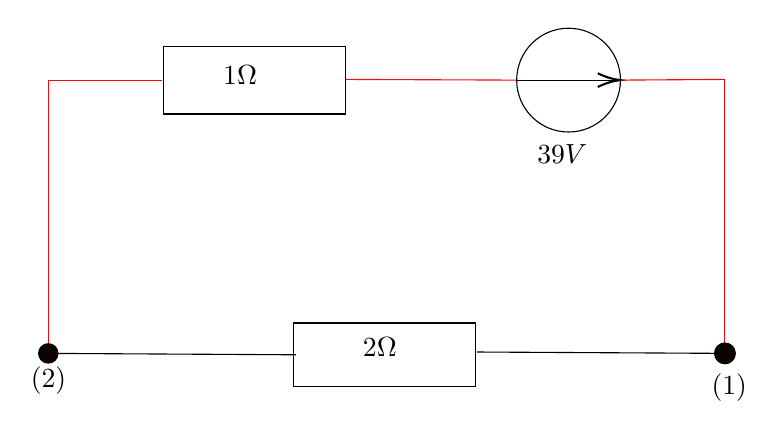
\begin{tikzpicture}[x=0.75pt,y=0.75pt,yscale=-1,xscale=1]
%uncomment if require: \path (0,300); %set diagram left start at 0, and has height of 300

%Straight Lines [id:da3224313797429348] 
\draw    (362.33,191.67) -- (481.67,192.33) ;
%Shape: Rectangle [id:dp6893354233123505] 
\draw   (273.67,177.67) -- (361.67,177.67) -- (361.67,208.33) -- (273.67,208.33) -- cycle ;
%Straight Lines [id:da9223439565409108] 
\draw    (155.67,192.33) -- (275,193) ;
%Straight Lines [id:da4026004964078189] 
\draw [color={rgb, 255:red, 249; green, 12; blue, 12 }  ,draw opacity=1 ]   (155.67,61) -- (155.67,192.33) ;
%Straight Lines [id:da7755220774610179] 
\draw [color={rgb, 255:red, 242; green, 8; blue, 8 }  ,draw opacity=1 ]   (481.67,60.33) -- (481.67,192.33) ;
%Shape: Rectangle [id:dp5308903226746371] 
\draw   (211,44.33) -- (299,44.33) -- (299,77) -- (211,77) -- cycle ;
%Shape: Circle [id:dp513529319607058] 
\draw   (381.33,60.67) .. controls (381.33,46.86) and (392.53,35.67) .. (406.33,35.67) .. controls (420.14,35.67) and (431.33,46.86) .. (431.33,60.67) .. controls (431.33,74.47) and (420.14,85.67) .. (406.33,85.67) .. controls (392.53,85.67) and (381.33,74.47) .. (381.33,60.67) -- cycle ;
%Straight Lines [id:da6344708178258509] 
\draw    (381.33,60.67) -- (429.33,60.67) ;
\draw [shift={(431.33,60.67)}, rotate = 180] [color={rgb, 255:red, 0; green, 0; blue, 0 }  ][line width=0.75]    (10.93,-3.29) .. controls (6.95,-1.4) and (3.31,-0.3) .. (0,0) .. controls (3.31,0.3) and (6.95,1.4) .. (10.93,3.29)   ;

%Straight Lines [id:da5413569904406206] 
\draw [color={rgb, 255:red, 247; green, 10; blue, 10 }  ,draw opacity=1 ]   (210.33,61) -- (155.67,61) ;
%Straight Lines [id:da9673200830998514] 
\draw [color={rgb, 255:red, 241; green, 18; blue, 18 }  ,draw opacity=1 ]   (299,60.33) -- (381.33,60.67) ;
%Straight Lines [id:da9317028525661359] 
\draw [color={rgb, 255:red, 244; green, 9; blue, 9 }  ,draw opacity=1 ]   (481.67,60.33) -- (431.33,60.67) ;
%Shape: Circle [id:dp19423452087766102] 
\draw  [fill={rgb, 255:red, 13; green, 1; blue, 1 }  ,fill opacity=1 ] (476.67,192.33) .. controls (476.67,189.57) and (478.91,187.33) .. (481.67,187.33) .. controls (484.43,187.33) and (486.67,189.57) .. (486.67,192.33) .. controls (486.67,195.09) and (484.43,197.33) .. (481.67,197.33) .. controls (478.91,197.33) and (476.67,195.09) .. (476.67,192.33) -- cycle ;
%Shape: Circle [id:dp6097035217414721] 
\draw  [fill={rgb, 255:red, 13; green, 1; blue, 1 }  ,fill opacity=1 ] (151,192.33) .. controls (151,189.76) and (153.09,187.67) .. (155.67,187.67) .. controls (158.24,187.67) and (160.33,189.76) .. (160.33,192.33) .. controls (160.33,194.91) and (158.24,197) .. (155.67,197) .. controls (153.09,197) and (151,194.91) .. (151,192.33) -- cycle ;

% Text Node
\draw (474,201) node [anchor=north west][inner sep=0.75pt]   [align=left] {(1)};
% Text Node
\draw (146,197.33) node [anchor=north west][inner sep=0.75pt]   [align=left] {(2)};
% Text Node
\draw (306,183.67) node [anchor=north west][inner sep=0.75pt]   [align=left] {$\displaystyle 2\si{\ohm}$};
% Text Node
\draw (238.67,52.33) node [anchor=north west][inner sep=0.75pt]   [align=left] {$\displaystyle 1\si{\ohm}$};
% Text Node
\draw (390,90.33) node [anchor=north west][inner sep=0.75pt]   [align=left] {$\displaystyle 39V$};


\end{tikzpicture}

\end{center}

\newpage

\subsection{Caracteristica rezistorului liniar și a generatorului echivalent}
Știm foarte bine că caracteristica generatorului liniar va fi o dreaptă cu pantă negativă unde sunt incluse perechile (Intensitate, Tensiune) - ($0$, $E_{ech}$) și ($I_{sc}$, $0$), deci curenentul de sarcină va varia între \textbf{0} și $I_{sc}$ (scurt circuit).

\begin{center}
    

\tikzset{every picture/.style={line width=0.75pt}} %set default line width to 0.75pt        

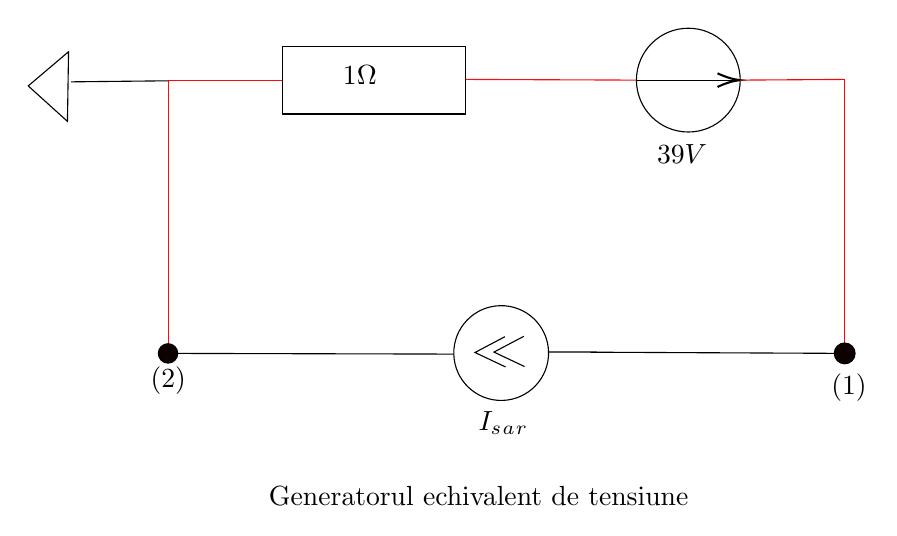
\begin{tikzpicture}[x=0.75pt,y=0.75pt,yscale=-1,xscale=1]
%uncomment if require: \path (0,300); %set diagram left start at 0, and has height of 300

%Straight Lines [id:da3224313797429348] 
\draw    (362.33,191.67) -- (338.99,191.66) -- (481.67,192.33) ;
%Straight Lines [id:da9223439565409108] 
\draw    (155.67,192.33) -- (293.34,192.67) ;
%Straight Lines [id:da4026004964078189] 
\draw [color={rgb, 255:red, 249; green, 12; blue, 12 }  ,draw opacity=1 ]   (155.67,61) -- (155.67,192.33) ;
%Straight Lines [id:da7755220774610179] 
\draw [color={rgb, 255:red, 242; green, 8; blue, 8 }  ,draw opacity=1 ]   (481.67,60.33) -- (481.67,192.33) ;
%Shape: Rectangle [id:dp5308903226746371] 
\draw   (211,44.33) -- (299,44.33) -- (299,77) -- (211,77) -- cycle ;
%Shape: Circle [id:dp513529319607058] 
\draw   (381.33,60.67) .. controls (381.33,46.86) and (392.53,35.67) .. (406.33,35.67) .. controls (420.14,35.67) and (431.33,46.86) .. (431.33,60.67) .. controls (431.33,74.47) and (420.14,85.67) .. (406.33,85.67) .. controls (392.53,85.67) and (381.33,74.47) .. (381.33,60.67) -- cycle ;
%Straight Lines [id:da6344708178258509] 
\draw    (381.33,60.67) -- (429.33,60.67) ;
\draw [shift={(431.33,60.67)}, rotate = 180] [color={rgb, 255:red, 0; green, 0; blue, 0 }  ][line width=0.75]    (10.93,-3.29) .. controls (6.95,-1.4) and (3.31,-0.3) .. (0,0) .. controls (3.31,0.3) and (6.95,1.4) .. (10.93,3.29)   ;

%Straight Lines [id:da5413569904406206] 
\draw [color={rgb, 255:red, 247; green, 10; blue, 10 }  ,draw opacity=1 ]   (210.33,61) -- (155.67,61) ;
%Straight Lines [id:da9673200830998514] 
\draw [color={rgb, 255:red, 241; green, 18; blue, 18 }  ,draw opacity=1 ]   (299,60.33) -- (381.33,60.67) ;
%Straight Lines [id:da9317028525661359] 
\draw [color={rgb, 255:red, 244; green, 9; blue, 9 }  ,draw opacity=1 ]   (481.67,60.33) -- (431.33,60.67) ;
%Shape: Circle [id:dp19423452087766102] 
\draw  [fill={rgb, 255:red, 13; green, 1; blue, 1 }  ,fill opacity=1 ] (476.67,192.33) .. controls (476.67,189.57) and (478.91,187.33) .. (481.67,187.33) .. controls (484.43,187.33) and (486.67,189.57) .. (486.67,192.33) .. controls (486.67,195.09) and (484.43,197.33) .. (481.67,197.33) .. controls (478.91,197.33) and (476.67,195.09) .. (476.67,192.33) -- cycle ;
%Shape: Circle [id:dp6097035217414721] 
\draw  [fill={rgb, 255:red, 13; green, 1; blue, 1 }  ,fill opacity=1 ] (151,192.33) .. controls (151,189.76) and (153.09,187.67) .. (155.67,187.67) .. controls (158.24,187.67) and (160.33,189.76) .. (160.33,192.33) .. controls (160.33,194.91) and (158.24,197) .. (155.67,197) .. controls (153.09,197) and (151,194.91) .. (151,192.33) -- cycle ;
%Shape: Triangle [id:dp846980856471538] 
\draw   (88.3,63.46) -- (107.73,46.99) -- (107.19,80.54) -- cycle ;
%Straight Lines [id:da11342624375809507] 
\draw    (109,61.5) -- (155.67,61) ;
%Flowchart: Connector [id:dp18193164024993602] 
\draw   (338.99,191.66) .. controls (339.27,204.27) and (329.28,214.72) .. (316.67,214.99) .. controls (304.06,215.27) and (293.62,205.28) .. (293.34,192.67) .. controls (293.06,180.06) and (303.06,169.62) .. (315.66,169.34) .. controls (328.27,169.06) and (338.72,179.06) .. (338.99,191.66) -- cycle ;
\draw   (327.4,198.66) -- (312.68,191.7) -- (327.08,184.1) ;
\draw   (318.27,198.86) -- (303.55,191.9) -- (317.95,184.3) ;


% Text Node
\draw (474,201) node [anchor=north west][inner sep=0.75pt]   [align=left] {(1)};
% Text Node
\draw (146,197.33) node [anchor=north west][inner sep=0.75pt]   [align=left] {(2)};
% Text Node
\draw (238.67,52.33) node [anchor=north west][inner sep=0.75pt]   [align=left] {$\displaystyle 1\si{\ohm}$};
% Text Node
\draw (390,90.33) node [anchor=north west][inner sep=0.75pt]   [align=left] {$\displaystyle 39V$};
% Text Node
\draw (304,219) node [anchor=north west][inner sep=0.75pt]   [align=left] {$\displaystyle I_{s}{}_{a}{}_{r}$};
% Text Node
\draw (203,255) node [anchor=north west][inner sep=0.75pt]   [align=left] {Generatorul echivalent de tensiune};


\end{tikzpicture}

\end{center}

Pentru a putea vedea caracteristica acestuia și pentru a nu supăra LTSpice-ul vom inițializa valaorea intensității de sarcină ca fiind 1, însă pentru a rula circuitul generatorului echivalent vom folosi operatorul \textbf{.dc}, unde vom varia intensitatea de sarcină de la 0 către intensitatea de scurtcircuit.

\begin{figure}[h]
    \centering
    \includegraphics[width=\linewidth, height=\textheight, keepaspectratio]{Caracteristica_generator.png}
    \label{fig:gener}
\end{figure}

Dacă dorim să interpretăm caracteristica rezistorului liniar vom avea nevoie să imprimăm prin acesta, aceiași intensitate de sarcină, pentru acest lucru vom avea nevoie de un \textbf{SICI}, însă un SICI are nevoie ca referință o sursă de tensiune, deci pentru a nu strica circuitele vom adăuga un SIT, în circuitul de mai sus orientat la fel ca $E_{ech}$, însă cu valoarea \textbf{0}. Ambele circuite vor avea ca referință același ground. Important este că factorul de transmitere la SICI să fie 1.

\begin{center}
    

\tikzset{every picture/.style={line width=0.75pt}} %set default line width to 0.75pt        

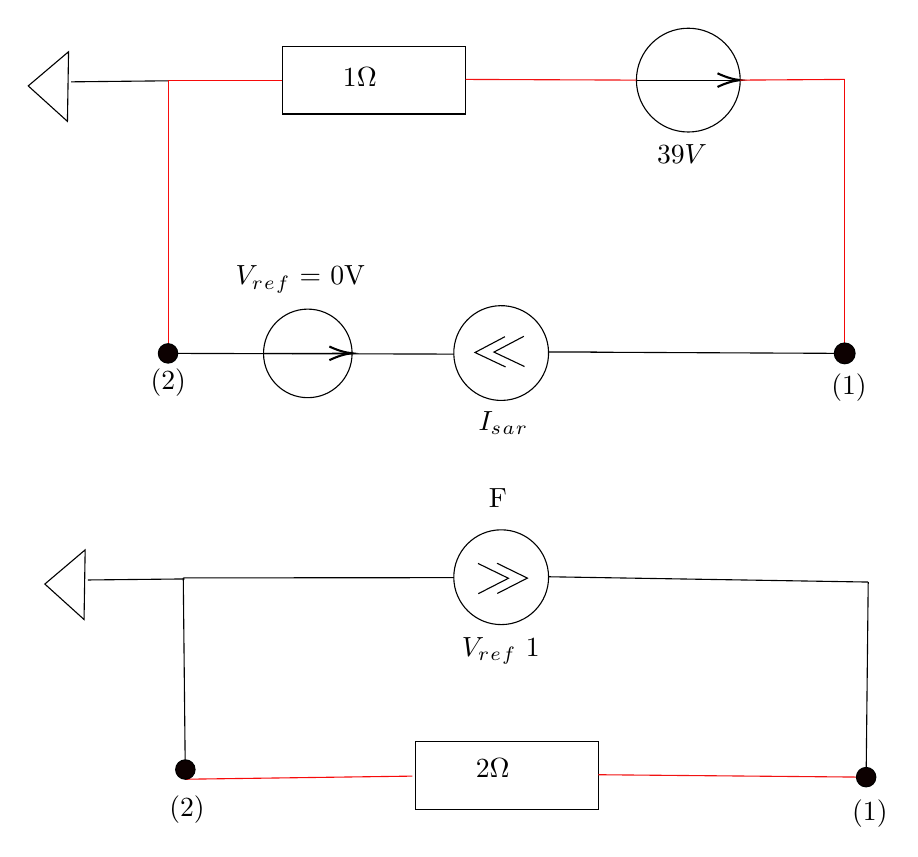
\begin{tikzpicture}[x=0.75pt,y=0.75pt,yscale=-1,xscale=1]
%uncomment if require: \path (0,471); %set diagram left start at 0, and has height of 471

%Straight Lines [id:da3224313797429348] 
\draw    (362.33,191.67) -- (338.99,191.66) -- (481.67,192.33) ;
%Straight Lines [id:da9223439565409108] 
\draw    (155.67,192.33) -- (293.34,192.67) ;
%Straight Lines [id:da4026004964078189] 
\draw [color={rgb, 255:red, 249; green, 12; blue, 12 }  ,draw opacity=1 ]   (155.67,61) -- (155.67,192.33) ;
%Straight Lines [id:da7755220774610179] 
\draw [color={rgb, 255:red, 242; green, 8; blue, 8 }  ,draw opacity=1 ]   (481.67,60.33) -- (481.67,192.33) ;
%Shape: Rectangle [id:dp5308903226746371] 
\draw   (211,44.33) -- (299,44.33) -- (299,77) -- (211,77) -- cycle ;
%Shape: Circle [id:dp513529319607058] 
\draw   (381.33,60.67) .. controls (381.33,46.86) and (392.53,35.67) .. (406.33,35.67) .. controls (420.14,35.67) and (431.33,46.86) .. (431.33,60.67) .. controls (431.33,74.47) and (420.14,85.67) .. (406.33,85.67) .. controls (392.53,85.67) and (381.33,74.47) .. (381.33,60.67) -- cycle ;
%Straight Lines [id:da6344708178258509] 
\draw    (381.33,60.67) -- (429.33,60.67) ;
\draw [shift={(431.33,60.67)}, rotate = 180] [color={rgb, 255:red, 0; green, 0; blue, 0 }  ][line width=0.75]    (10.93,-3.29) .. controls (6.95,-1.4) and (3.31,-0.3) .. (0,0) .. controls (3.31,0.3) and (6.95,1.4) .. (10.93,3.29)   ;

%Straight Lines [id:da5413569904406206] 
\draw [color={rgb, 255:red, 247; green, 10; blue, 10 }  ,draw opacity=1 ]   (210.33,61) -- (155.67,61) ;
%Straight Lines [id:da9673200830998514] 
\draw [color={rgb, 255:red, 241; green, 18; blue, 18 }  ,draw opacity=1 ]   (299,60.33) -- (381.33,60.67) ;
%Straight Lines [id:da9317028525661359] 
\draw [color={rgb, 255:red, 244; green, 9; blue, 9 }  ,draw opacity=1 ]   (481.67,60.33) -- (431.33,60.67) ;
%Shape: Circle [id:dp19423452087766102] 
\draw  [fill={rgb, 255:red, 13; green, 1; blue, 1 }  ,fill opacity=1 ] (476.67,192.33) .. controls (476.67,189.57) and (478.91,187.33) .. (481.67,187.33) .. controls (484.43,187.33) and (486.67,189.57) .. (486.67,192.33) .. controls (486.67,195.09) and (484.43,197.33) .. (481.67,197.33) .. controls (478.91,197.33) and (476.67,195.09) .. (476.67,192.33) -- cycle ;
%Shape: Circle [id:dp6097035217414721] 
\draw  [fill={rgb, 255:red, 13; green, 1; blue, 1 }  ,fill opacity=1 ] (151,192.33) .. controls (151,189.76) and (153.09,187.67) .. (155.67,187.67) .. controls (158.24,187.67) and (160.33,189.76) .. (160.33,192.33) .. controls (160.33,194.91) and (158.24,197) .. (155.67,197) .. controls (153.09,197) and (151,194.91) .. (151,192.33) -- cycle ;
%Shape: Triangle [id:dp846980856471538] 
\draw   (88.3,63.46) -- (107.73,46.99) -- (107.19,80.54) -- cycle ;
%Straight Lines [id:da11342624375809507] 
\draw    (109,61.5) -- (155.67,61) ;
%Flowchart: Connector [id:dp18193164024993602] 
\draw   (338.99,191.66) .. controls (339.27,204.27) and (329.28,214.72) .. (316.67,214.99) .. controls (304.06,215.27) and (293.62,205.28) .. (293.34,192.67) .. controls (293.06,180.06) and (303.06,169.62) .. (315.66,169.34) .. controls (328.27,169.06) and (338.72,179.06) .. (338.99,191.66) -- cycle ;
\draw   (327.4,198.66) -- (312.68,191.7) -- (327.08,184.1) ;
\draw   (318.27,198.86) -- (303.55,191.9) -- (317.95,184.3) ;

%Flowchart: Connector [id:dp39634155556626394] 
\draw   (201.67,192.41) .. controls (201.62,180.63) and (211.14,171.04) .. (222.92,171) .. controls (234.7,170.96) and (244.29,180.47) .. (244.33,192.26) .. controls (244.38,204.04) and (234.86,213.62) .. (223.08,213.67) .. controls (211.3,213.71) and (201.71,204.19) .. (201.67,192.41) -- cycle ;
%Straight Lines [id:da8046356779505501] 
\draw    (201.67,192.41) -- (242.33,192.26) ;
\draw [shift={(244.33,192.26)}, rotate = 179.79] [color={rgb, 255:red, 0; green, 0; blue, 0 }  ][line width=0.75]    (10.93,-3.29) .. controls (6.95,-1.4) and (3.31,-0.3) .. (0,0) .. controls (3.31,0.3) and (6.95,1.4) .. (10.93,3.29)   ;

%Shape: Rectangle [id:dp9347282647130384] 
\draw   (275,379.33) -- (363,379.33) -- (363,412) -- (275,412) -- cycle ;
%Straight Lines [id:da46063920757329946] 
\draw [color={rgb, 255:red, 247; green, 10; blue, 10 }  ,draw opacity=1 ]   (273.33,396) -- (164,397.5) ;
%Straight Lines [id:da9524819149878361] 
\draw [color={rgb, 255:red, 241; green, 18; blue, 18 }  ,draw opacity=1 ]   (363,395.33) -- (492,396.5) ;
%Flowchart: Connector [id:dp5947007780675961] 
\draw   (293.33,300.38) .. controls (293.22,287.77) and (303.34,277.45) .. (315.95,277.33) .. controls (328.56,277.22) and (338.88,287.34) .. (339,299.95) .. controls (339.12,312.56) and (328.99,322.88) .. (316.38,323) .. controls (303.77,323.12) and (293.45,312.99) .. (293.33,300.38) -- cycle ;
\draw   (305.01,293.53) -- (319.65,300.68) -- (305.15,308.1) ;
\draw   (314.15,293.44) -- (328.78,300.59) -- (314.28,308.01) ;

%Straight Lines [id:da07761832432547755] 
\draw    (163,300.5) -- (293.33,300.38) ;
%Straight Lines [id:da30601144701094873] 
\draw    (164,397.5) -- (163,300.5) ;
%Straight Lines [id:da3830418127277402] 
\draw    (493,302.5) -- (339,299.95) ;
%Straight Lines [id:da7341863531791317] 
\draw    (493,302.5) -- (492,396.5) ;
%Shape: Triangle [id:dp9759803153968614] 
\draw   (96.3,303.46) -- (115.73,286.99) -- (115.19,320.54) -- cycle ;
%Straight Lines [id:da8772917186623932] 
\draw    (117,301.5) -- (163.67,301) ;
%Shape: Circle [id:dp18201587172567524] 
\draw  [fill={rgb, 255:red, 13; green, 1; blue, 1 }  ,fill opacity=1 ] (159.33,392.83) .. controls (159.33,390.26) and (161.42,388.17) .. (164,388.17) .. controls (166.58,388.17) and (168.67,390.26) .. (168.67,392.83) .. controls (168.67,395.41) and (166.58,397.5) .. (164,397.5) .. controls (161.42,397.5) and (159.33,395.41) .. (159.33,392.83) -- cycle ;
%Shape: Circle [id:dp39806425142833923] 
\draw  [fill={rgb, 255:red, 13; green, 1; blue, 1 }  ,fill opacity=1 ] (487.33,396.5) .. controls (487.33,393.92) and (489.42,391.83) .. (492,391.83) .. controls (494.58,391.83) and (496.67,393.92) .. (496.67,396.5) .. controls (496.67,399.08) and (494.58,401.17) .. (492,401.17) .. controls (489.42,401.17) and (487.33,399.08) .. (487.33,396.5) -- cycle ;

% Text Node
\draw (474,201) node [anchor=north west][inner sep=0.75pt]   [align=left] {(1)};
% Text Node
\draw (146,198.33) node [anchor=north west][inner sep=0.75pt]   [align=left] {(2)};
% Text Node
\draw (238.67,53.33) node [anchor=north west][inner sep=0.75pt]   [align=left] {$\displaystyle 1\si{\ohm}$};
% Text Node
\draw (390,90.33) node [anchor=north west][inner sep=0.75pt]   [align=left] {$\displaystyle 39V$};
% Text Node
\draw (304,219) node [anchor=north west][inner sep=0.75pt]   [align=left] {$\displaystyle I_{s}{}_{a}{}_{r}$};
% Text Node
\draw (187,149) node [anchor=north west][inner sep=0.75pt]   [align=left] {$\displaystyle V_{r}{}_{e}{}_{f}$ = 0V};
% Text Node
\draw (302.67,386.33) node [anchor=north west][inner sep=0.75pt]   [align=left] {$\displaystyle 2\si{\ohm}$};
% Text Node
\draw (309,256) node [anchor=north west][inner sep=0.75pt]   [align=left] {F};
% Text Node
\draw (296,328) node [anchor=north west][inner sep=0.75pt]   [align=left] {$\displaystyle V_{r}{}_{e}{}_{f}$ 1};
% Text Node
\draw (484,406) node [anchor=north west][inner sep=0.75pt]   [align=left] {(1)};
% Text Node
\draw (155,404.33) node [anchor=north west][inner sep=0.75pt]   [align=left] {(2)};


\end{tikzpicture}

\end{center}

Acum pentru a vizualiza caracteristicele acestora pe un singur graf ne vom folosi de LTSpice, iar pentru a determina care este punctul static de funcționare vom selecta perechea ce definește intersecția celor două grafice, altfel spus haideți să trecem la treabă !!!
\newpage

\begin{figure}[h]
    \centering
    \includegraphics[width=\linewidth, height=\textheight, keepaspectratio]{Caracteristica_ambele.png}
    \caption{Caracteristici și Punctul stabil}
    \label{fig:ambele}
\end{figure}

\vspace{2cm}
Deci spre final de această secțiune am văzut care este caracteristica generatorului echivalent de tensiune și caracteristica rezistorului liniar, față de restul circuitului la care este conectat. Totodată am aflat și punctul static de funcționare care este determinat de perechea de intensitate și tensiune (13.092, 25.907).

\vspace{2cm}
În următoarele două secțiuni vom vedea ce se întâmplă atunci când înlocuim rezistorul liniar cu o diodă Zener prin două metode, cea directă și cea indirectă și la fel vom afla punctele statice de funcționare, cât și caracteristicile fiecăreia.
\newpage

\subsection{Dioda Zener polarizată direct}
Pentru această secțiune vom înlocui în schemele de mai sus în loc de rezitorul liniar o diodă Zener polarizată direct. Știm foarte bine că dioda Zener lucrează ca un \textbf{SWITCH} pentru un circuit. Deci pe caracteristica acestuia vom vedea că dioda se deschide la o anumită tensiune $U_z$ numită tensiunea \emph{Zener} și apoi ideal ar trebui să fie o linie paralelă până la infinit, însă în cazul real aceasta are o dependență exponențială crescătoare, ceea ce vom observa și pe graficile următoare.

\begin{center}


\tikzset{every picture/.style={line width=0.75pt}} %set default line width to 0.75pt        

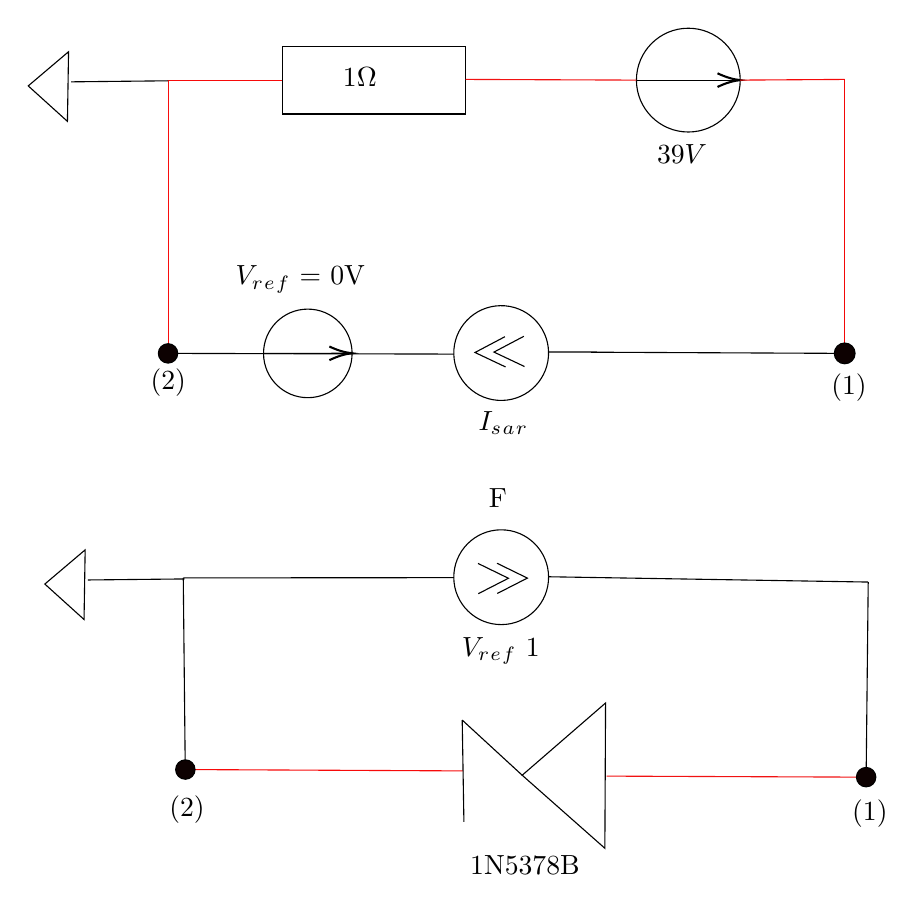
\begin{tikzpicture}[x=0.75pt,y=0.75pt,yscale=-1,xscale=1]
%uncomment if require: \path (0,471); %set diagram left start at 0, and has height of 471

%Straight Lines [id:da3224313797429348] 
\draw    (362.33,191.67) -- (338.99,191.66) -- (481.67,192.33) ;
%Straight Lines [id:da9223439565409108] 
\draw    (155.67,192.33) -- (293.34,192.67) ;
%Straight Lines [id:da4026004964078189] 
\draw [color={rgb, 255:red, 249; green, 12; blue, 12 }  ,draw opacity=1 ]   (155.67,61) -- (155.67,192.33) ;
%Straight Lines [id:da7755220774610179] 
\draw [color={rgb, 255:red, 242; green, 8; blue, 8 }  ,draw opacity=1 ]   (481.67,60.33) -- (481.67,192.33) ;
%Shape: Rectangle [id:dp5308903226746371] 
\draw   (211,44.33) -- (299,44.33) -- (299,77) -- (211,77) -- cycle ;
%Shape: Circle [id:dp513529319607058] 
\draw   (381.33,60.67) .. controls (381.33,46.86) and (392.53,35.67) .. (406.33,35.67) .. controls (420.14,35.67) and (431.33,46.86) .. (431.33,60.67) .. controls (431.33,74.47) and (420.14,85.67) .. (406.33,85.67) .. controls (392.53,85.67) and (381.33,74.47) .. (381.33,60.67) -- cycle ;
%Straight Lines [id:da6344708178258509] 
\draw    (381.33,60.67) -- (429.33,60.67) ;
\draw [shift={(431.33,60.67)}, rotate = 180] [color={rgb, 255:red, 0; green, 0; blue, 0 }  ][line width=0.75]    (10.93,-3.29) .. controls (6.95,-1.4) and (3.31,-0.3) .. (0,0) .. controls (3.31,0.3) and (6.95,1.4) .. (10.93,3.29)   ;

%Straight Lines [id:da5413569904406206] 
\draw [color={rgb, 255:red, 247; green, 10; blue, 10 }  ,draw opacity=1 ]   (210.33,61) -- (155.67,61) ;
%Straight Lines [id:da9673200830998514] 
\draw [color={rgb, 255:red, 241; green, 18; blue, 18 }  ,draw opacity=1 ]   (299,60.33) -- (381.33,60.67) ;
%Straight Lines [id:da9317028525661359] 
\draw [color={rgb, 255:red, 244; green, 9; blue, 9 }  ,draw opacity=1 ]   (481.67,60.33) -- (431.33,60.67) ;
%Shape: Circle [id:dp19423452087766102] 
\draw  [fill={rgb, 255:red, 13; green, 1; blue, 1 }  ,fill opacity=1 ] (476.67,192.33) .. controls (476.67,189.57) and (478.91,187.33) .. (481.67,187.33) .. controls (484.43,187.33) and (486.67,189.57) .. (486.67,192.33) .. controls (486.67,195.09) and (484.43,197.33) .. (481.67,197.33) .. controls (478.91,197.33) and (476.67,195.09) .. (476.67,192.33) -- cycle ;
%Shape: Circle [id:dp6097035217414721] 
\draw  [fill={rgb, 255:red, 13; green, 1; blue, 1 }  ,fill opacity=1 ] (151,192.33) .. controls (151,189.76) and (153.09,187.67) .. (155.67,187.67) .. controls (158.24,187.67) and (160.33,189.76) .. (160.33,192.33) .. controls (160.33,194.91) and (158.24,197) .. (155.67,197) .. controls (153.09,197) and (151,194.91) .. (151,192.33) -- cycle ;
%Shape: Triangle [id:dp846980856471538] 
\draw   (88.3,63.46) -- (107.73,46.99) -- (107.19,80.54) -- cycle ;
%Straight Lines [id:da11342624375809507] 
\draw    (109,61.5) -- (155.67,61) ;
%Flowchart: Connector [id:dp18193164024993602] 
\draw   (338.99,191.66) .. controls (339.27,204.27) and (329.28,214.72) .. (316.67,214.99) .. controls (304.06,215.27) and (293.62,205.28) .. (293.34,192.67) .. controls (293.06,180.06) and (303.06,169.62) .. (315.66,169.34) .. controls (328.27,169.06) and (338.72,179.06) .. (338.99,191.66) -- cycle ;
\draw   (327.4,198.66) -- (312.68,191.7) -- (327.08,184.1) ;
\draw   (318.27,198.86) -- (303.55,191.9) -- (317.95,184.3) ;

%Flowchart: Connector [id:dp39634155556626394] 
\draw   (201.67,192.41) .. controls (201.62,180.63) and (211.14,171.04) .. (222.92,171) .. controls (234.7,170.96) and (244.29,180.47) .. (244.33,192.26) .. controls (244.38,204.04) and (234.86,213.62) .. (223.08,213.67) .. controls (211.3,213.71) and (201.71,204.19) .. (201.67,192.41) -- cycle ;
%Straight Lines [id:da8046356779505501] 
\draw    (201.67,192.41) -- (242.33,192.26) ;
\draw [shift={(244.33,192.26)}, rotate = 179.79] [color={rgb, 255:red, 0; green, 0; blue, 0 }  ][line width=0.75]    (10.93,-3.29) .. controls (6.95,-1.4) and (3.31,-0.3) .. (0,0) .. controls (3.31,0.3) and (6.95,1.4) .. (10.93,3.29)   ;

%Straight Lines [id:da555814560200085] 
\draw [color={rgb, 255:red, 247; green, 10; blue, 10 }  ,draw opacity=1 ]   (297.8,393.49) -- (164,392.83) ;
%Shape: Triangle [id:dp2601732593806676] 
\draw   (326.29,395.57) -- (366.46,360.77) -- (366.12,430.77) -- cycle ;
%Straight Lines [id:da46077510576058867] 
\draw    (297.39,368.99) -- (326.29,395.57) ;
%Straight Lines [id:da26664143203637125] 
\draw    (298.21,417.99) -- (297.39,368.99) ;

%Straight Lines [id:da9524819149878361] 
\draw [color={rgb, 255:red, 241; green, 18; blue, 18 }  ,draw opacity=1 ]   (367,396) -- (492,396.5) ;
%Flowchart: Connector [id:dp5947007780675961] 
\draw   (293.33,300.38) .. controls (293.22,287.77) and (303.34,277.45) .. (315.95,277.33) .. controls (328.56,277.22) and (338.88,287.34) .. (339,299.95) .. controls (339.12,312.56) and (328.99,322.88) .. (316.38,323) .. controls (303.77,323.12) and (293.45,312.99) .. (293.33,300.38) -- cycle ;
\draw   (305.01,293.53) -- (319.65,300.68) -- (305.15,308.1) ;
\draw   (314.15,293.44) -- (328.78,300.59) -- (314.28,308.01) ;

%Straight Lines [id:da07761832432547755] 
\draw    (163,300.5) -- (293.33,300.38) ;
%Straight Lines [id:da30601144701094873] 
\draw    (164,397.5) -- (163,300.5) ;
%Straight Lines [id:da3830418127277402] 
\draw    (493,302.5) -- (339,299.95) ;
%Straight Lines [id:da7341863531791317] 
\draw    (493,302.5) -- (492,396.5) ;
%Shape: Triangle [id:dp9759803153968614] 
\draw   (96.3,303.46) -- (115.73,286.99) -- (115.19,320.54) -- cycle ;
%Straight Lines [id:da8772917186623932] 
\draw    (117,301.5) -- (163.67,301) ;
%Shape: Circle [id:dp18201587172567524] 
\draw  [fill={rgb, 255:red, 13; green, 1; blue, 1 }  ,fill opacity=1 ] (159.33,392.83) .. controls (159.33,390.26) and (161.42,388.17) .. (164,388.17) .. controls (166.58,388.17) and (168.67,390.26) .. (168.67,392.83) .. controls (168.67,395.41) and (166.58,397.5) .. (164,397.5) .. controls (161.42,397.5) and (159.33,395.41) .. (159.33,392.83) -- cycle ;
%Shape: Circle [id:dp39806425142833923] 
\draw  [fill={rgb, 255:red, 13; green, 1; blue, 1 }  ,fill opacity=1 ] (487.33,396.5) .. controls (487.33,393.92) and (489.42,391.83) .. (492,391.83) .. controls (494.58,391.83) and (496.67,393.92) .. (496.67,396.5) .. controls (496.67,399.08) and (494.58,401.17) .. (492,401.17) .. controls (489.42,401.17) and (487.33,399.08) .. (487.33,396.5) -- cycle ;

% Text Node
\draw (474,201) node [anchor=north west][inner sep=0.75pt]   [align=left] {(1)};
% Text Node
\draw (146,198.33) node [anchor=north west][inner sep=0.75pt]   [align=left] {(2)};
% Text Node
\draw (238.67,53.33) node [anchor=north west][inner sep=0.75pt]   [align=left] {$\displaystyle 1\si{\ohm}$};
% Text Node
\draw (390,90.33) node [anchor=north west][inner sep=0.75pt]   [align=left] {$\displaystyle 39V$};
% Text Node
\draw (304,219) node [anchor=north west][inner sep=0.75pt]   [align=left] {$\displaystyle I_{s}{}_{a}{}_{r}$};
% Text Node
\draw (187,149) node [anchor=north west][inner sep=0.75pt]   [align=left] {$\displaystyle V_{r}{}_{e}{}_{f}$ = 0V};
% Text Node
\draw (309,256) node [anchor=north west][inner sep=0.75pt]   [align=left] {F};
% Text Node
\draw (296,328) node [anchor=north west][inner sep=0.75pt]   [align=left] {$\displaystyle V_{r}{}_{e}{}_{f}$ 1};
% Text Node
\draw (484,406) node [anchor=north west][inner sep=0.75pt]   [align=left] {(1)};
% Text Node
\draw (155,404.33) node [anchor=north west][inner sep=0.75pt]   [align=left] {(2)};
% Text Node
\draw (122,267.67) node [anchor=north west][inner sep=0.75pt]   [align=left] {};
% Text Node
\draw (299.96,432.98) node [anchor=north west][inner sep=0.75pt]   [align=left] {1N5378B};


\end{tikzpicture}



\end{center}

Dioda Zener care a fost aleasă pentru a mulțumi LTSpice-ul este \emph{1N5378B}, care are "\textbf{breakdown voltage}" egal cu \textbf{100V}, care este mai mare decât tensiunea echivalentă a generatorului echivalent de tensiune $E_{ech} = 39V$.

\newpage

\begin{figure}[h]
    \centering
    \includegraphics[width=\linewidth, height=\textheight, keepaspectratio]{Dioda_direct.png}
    \caption{Caracteristica diodei Zener polarizată direct}
    \label{fig:direct}
\end{figure}

\vspace{2cm}
După cum putem observa pe graficul de mai sus, dioda Zener aleasă are o tensiune de deschidere de \textbf{922mV} prin preajma intensității cu valoarea 0, iar punctul stabil de funcționare este defapt intersecția graficului diodei cu graficul generatorului, adică determinat de perechea (Intensitate, Tensiune) $\approx$ (34.5A, 4.6V). Un lucru foarte important de menționat este că dioda Zener pentru modelul ideal ar trebui să fie dependent constant față de tensiunea de tensiunea de deschidere, adică să fie paralel cu axa intensității, însă în modelul real aceasta are o dependență exponențială crescătoare, fin această cauză putem observa pe grafic o creștere latentă a tensiunii. În caz că am fi ales o diodă Zener pentru care \textbf{breakdown voltage} ar fi fost mai mică decât tensiunea electromotoare, atunci această dependență de creștere exponențială pe cazul real, ar fi fost cu mult mai mare, din acest motiv am și ales această diodă cu o tensiunea mai mare decăt tensiunea generatorului.

\newpage

\subsection{Dioda Zener polarizată indirect}
Pentru această secțiune vom proceda identic ca la secțiunea anterioară însă vom schimba sensul diodei și pentru la fel a nu avea mari dependențe exponențiale a diodei, vom alege un \textbf{breakdown voltage} mai mic decît tensiunea electromotoare. Acestea fiind spuse vom alege dioda Zener \textbf{EDZV33B}, care are tensiunea de deschidere de 33V.

\vspace{3cm}

\begin{center}
    

\tikzset{every picture/.style={line width=0.75pt}} %set default line width to 0.75pt        

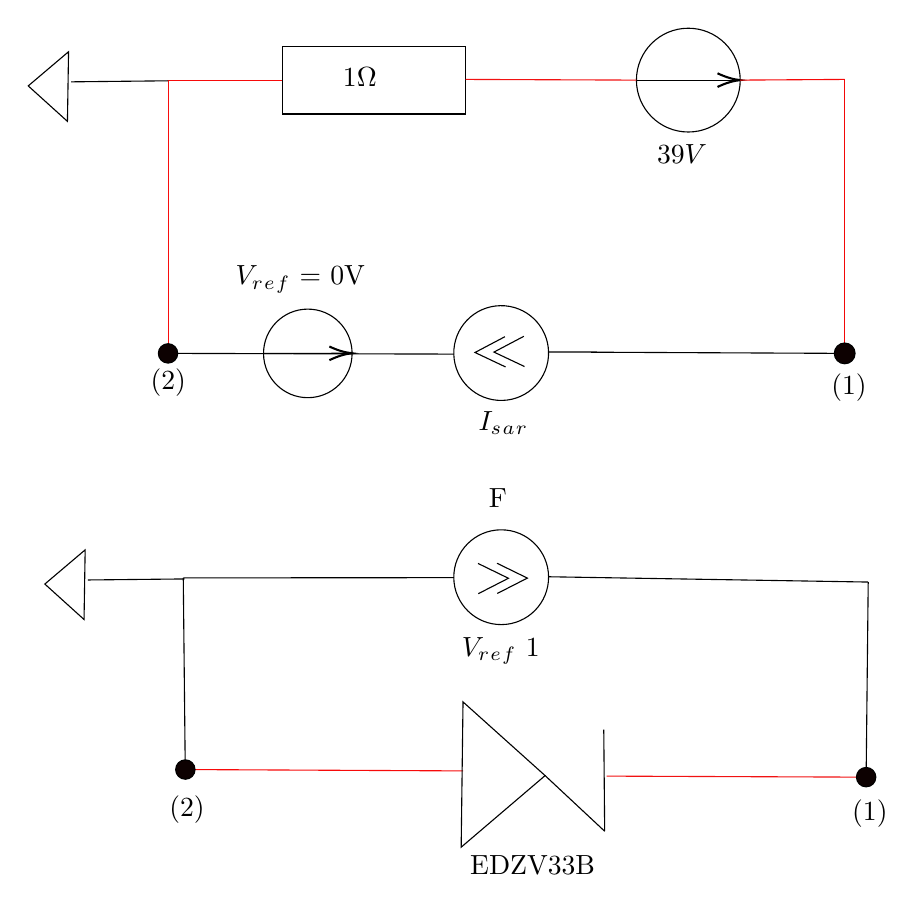
\begin{tikzpicture}[x=0.75pt,y=0.75pt,yscale=-1,xscale=1]
%uncomment if require: \path (0,471); %set diagram left start at 0, and has height of 471

%Straight Lines [id:da3224313797429348] 
\draw    (362.33,191.67) -- (338.99,191.66) -- (481.67,192.33) ;
%Straight Lines [id:da9223439565409108] 
\draw    (155.67,192.33) -- (293.34,192.67) ;
%Straight Lines [id:da4026004964078189] 
\draw [color={rgb, 255:red, 249; green, 12; blue, 12 }  ,draw opacity=1 ]   (155.67,61) -- (155.67,192.33) ;
%Straight Lines [id:da7755220774610179] 
\draw [color={rgb, 255:red, 242; green, 8; blue, 8 }  ,draw opacity=1 ]   (481.67,60.33) -- (481.67,192.33) ;
%Shape: Rectangle [id:dp5308903226746371] 
\draw   (211,44.33) -- (299,44.33) -- (299,77) -- (211,77) -- cycle ;
%Shape: Circle [id:dp513529319607058] 
\draw   (381.33,60.67) .. controls (381.33,46.86) and (392.53,35.67) .. (406.33,35.67) .. controls (420.14,35.67) and (431.33,46.86) .. (431.33,60.67) .. controls (431.33,74.47) and (420.14,85.67) .. (406.33,85.67) .. controls (392.53,85.67) and (381.33,74.47) .. (381.33,60.67) -- cycle ;
%Straight Lines [id:da6344708178258509] 
\draw    (381.33,60.67) -- (429.33,60.67) ;
\draw [shift={(431.33,60.67)}, rotate = 180] [color={rgb, 255:red, 0; green, 0; blue, 0 }  ][line width=0.75]    (10.93,-3.29) .. controls (6.95,-1.4) and (3.31,-0.3) .. (0,0) .. controls (3.31,0.3) and (6.95,1.4) .. (10.93,3.29)   ;

%Straight Lines [id:da5413569904406206] 
\draw [color={rgb, 255:red, 247; green, 10; blue, 10 }  ,draw opacity=1 ]   (210.33,61) -- (155.67,61) ;
%Straight Lines [id:da9673200830998514] 
\draw [color={rgb, 255:red, 241; green, 18; blue, 18 }  ,draw opacity=1 ]   (299,60.33) -- (381.33,60.67) ;
%Straight Lines [id:da9317028525661359] 
\draw [color={rgb, 255:red, 244; green, 9; blue, 9 }  ,draw opacity=1 ]   (481.67,60.33) -- (431.33,60.67) ;
%Shape: Circle [id:dp19423452087766102] 
\draw  [fill={rgb, 255:red, 13; green, 1; blue, 1 }  ,fill opacity=1 ] (476.67,192.33) .. controls (476.67,189.57) and (478.91,187.33) .. (481.67,187.33) .. controls (484.43,187.33) and (486.67,189.57) .. (486.67,192.33) .. controls (486.67,195.09) and (484.43,197.33) .. (481.67,197.33) .. controls (478.91,197.33) and (476.67,195.09) .. (476.67,192.33) -- cycle ;
%Shape: Circle [id:dp6097035217414721] 
\draw  [fill={rgb, 255:red, 13; green, 1; blue, 1 }  ,fill opacity=1 ] (151,192.33) .. controls (151,189.76) and (153.09,187.67) .. (155.67,187.67) .. controls (158.24,187.67) and (160.33,189.76) .. (160.33,192.33) .. controls (160.33,194.91) and (158.24,197) .. (155.67,197) .. controls (153.09,197) and (151,194.91) .. (151,192.33) -- cycle ;
%Shape: Triangle [id:dp846980856471538] 
\draw   (88.3,63.46) -- (107.73,46.99) -- (107.19,80.54) -- cycle ;
%Straight Lines [id:da11342624375809507] 
\draw    (109,61.5) -- (155.67,61) ;
%Flowchart: Connector [id:dp18193164024993602] 
\draw   (338.99,191.66) .. controls (339.27,204.27) and (329.28,214.72) .. (316.67,214.99) .. controls (304.06,215.27) and (293.62,205.28) .. (293.34,192.67) .. controls (293.06,180.06) and (303.06,169.62) .. (315.66,169.34) .. controls (328.27,169.06) and (338.72,179.06) .. (338.99,191.66) -- cycle ;
\draw   (327.4,198.66) -- (312.68,191.7) -- (327.08,184.1) ;
\draw   (318.27,198.86) -- (303.55,191.9) -- (317.95,184.3) ;

%Flowchart: Connector [id:dp39634155556626394] 
\draw   (201.67,192.41) .. controls (201.62,180.63) and (211.14,171.04) .. (222.92,171) .. controls (234.7,170.96) and (244.29,180.47) .. (244.33,192.26) .. controls (244.38,204.04) and (234.86,213.62) .. (223.08,213.67) .. controls (211.3,213.71) and (201.71,204.19) .. (201.67,192.41) -- cycle ;
%Straight Lines [id:da8046356779505501] 
\draw    (201.67,192.41) -- (242.33,192.26) ;
\draw [shift={(244.33,192.26)}, rotate = 179.79] [color={rgb, 255:red, 0; green, 0; blue, 0 }  ][line width=0.75]    (10.93,-3.29) .. controls (6.95,-1.4) and (3.31,-0.3) .. (0,0) .. controls (3.31,0.3) and (6.95,1.4) .. (10.93,3.29)   ;

%Straight Lines [id:da555814560200085] 
\draw [color={rgb, 255:red, 247; green, 10; blue, 10 }  ,draw opacity=1 ]   (297.8,393.49) -- (164,392.83) ;
%Shape: Triangle [id:dp2601732593806676] 
\draw   (337.33,395.75) -- (296.89,430.24) -- (297.78,360.25) -- cycle ;
%Straight Lines [id:da46077510576058867] 
\draw    (366.03,422.56) -- (337.33,395.75) ;
%Straight Lines [id:da26664143203637125] 
\draw    (365.59,373.55) -- (366.03,422.56) ;

%Straight Lines [id:da9524819149878361] 
\draw [color={rgb, 255:red, 241; green, 18; blue, 18 }  ,draw opacity=1 ]   (367,396) -- (492,396.5) ;
%Flowchart: Connector [id:dp5947007780675961] 
\draw   (293.33,300.38) .. controls (293.22,287.77) and (303.34,277.45) .. (315.95,277.33) .. controls (328.56,277.22) and (338.88,287.34) .. (339,299.95) .. controls (339.12,312.56) and (328.99,322.88) .. (316.38,323) .. controls (303.77,323.12) and (293.45,312.99) .. (293.33,300.38) -- cycle ;
\draw   (305.01,293.53) -- (319.65,300.68) -- (305.15,308.1) ;
\draw   (314.15,293.44) -- (328.78,300.59) -- (314.28,308.01) ;

%Straight Lines [id:da07761832432547755] 
\draw    (163,300.5) -- (293.33,300.38) ;
%Straight Lines [id:da30601144701094873] 
\draw    (164,397.5) -- (163,300.5) ;
%Straight Lines [id:da3830418127277402] 
\draw    (493,302.5) -- (339,299.95) ;
%Straight Lines [id:da7341863531791317] 
\draw    (493,302.5) -- (492,396.5) ;
%Shape: Triangle [id:dp9759803153968614] 
\draw   (96.3,303.46) -- (115.73,286.99) -- (115.19,320.54) -- cycle ;
%Straight Lines [id:da8772917186623932] 
\draw    (117,301.5) -- (163.67,301) ;
%Shape: Circle [id:dp18201587172567524] 
\draw  [fill={rgb, 255:red, 13; green, 1; blue, 1 }  ,fill opacity=1 ] (159.33,392.83) .. controls (159.33,390.26) and (161.42,388.17) .. (164,388.17) .. controls (166.58,388.17) and (168.67,390.26) .. (168.67,392.83) .. controls (168.67,395.41) and (166.58,397.5) .. (164,397.5) .. controls (161.42,397.5) and (159.33,395.41) .. (159.33,392.83) -- cycle ;
%Shape: Circle [id:dp39806425142833923] 
\draw  [fill={rgb, 255:red, 13; green, 1; blue, 1 }  ,fill opacity=1 ] (487.33,396.5) .. controls (487.33,393.92) and (489.42,391.83) .. (492,391.83) .. controls (494.58,391.83) and (496.67,393.92) .. (496.67,396.5) .. controls (496.67,399.08) and (494.58,401.17) .. (492,401.17) .. controls (489.42,401.17) and (487.33,399.08) .. (487.33,396.5) -- cycle ;

% Text Node
\draw (474,201) node [anchor=north west][inner sep=0.75pt]   [align=left] {(1)};
% Text Node
\draw (146,198.33) node [anchor=north west][inner sep=0.75pt]   [align=left] {(2)};
% Text Node
\draw (238.67,53.33) node [anchor=north west][inner sep=0.75pt]   [align=left] {$\displaystyle 1\si{\ohm}$};
% Text Node
\draw (390,90.33) node [anchor=north west][inner sep=0.75pt]   [align=left] {$\displaystyle 39V$};
% Text Node
\draw (304,219) node [anchor=north west][inner sep=0.75pt]   [align=left] {$\displaystyle I_{s}{}_{a}{}_{r}$};
% Text Node
\draw (187,149) node [anchor=north west][inner sep=0.75pt]   [align=left] {$\displaystyle V_{r}{}_{e}{}_{f}$ = 0V};
% Text Node
\draw (309,256) node [anchor=north west][inner sep=0.75pt]   [align=left] {F};
% Text Node
\draw (296,328) node [anchor=north west][inner sep=0.75pt]   [align=left] {$\displaystyle V_{r}{}_{e}{}_{f}$ 1};
% Text Node
\draw (484,406) node [anchor=north west][inner sep=0.75pt]   [align=left] {(1)};
% Text Node
\draw (155,404.33) node [anchor=north west][inner sep=0.75pt]   [align=left] {(2)};
% Text Node
\draw (122,267.67) node [anchor=north west][inner sep=0.75pt]   [align=left] {};
% Text Node
\draw (299.96,432.98) node [anchor=north west][inner sep=0.75pt]   [align=left] {EDZV33B};


\end{tikzpicture}

\end{center}
\newpage

\begin{figure}[h]
    \centering
    \includegraphics[width=\linewidth, height=\textheight, keepaspectratio]{Dioda_indirect.png}
    \caption{Caracteristica diodei Zener polarizată indirect}
    \label{fig:indirect}
\end{figure}

\vspace{3cm}
După cum putem observa și pe graficul de mai sus, dioda Zener în modelul real se deschide la o tensiune aproximativ egală cu \textbf{33V} în preajma curentului egal cu 0 și cum suntem pe modelul real aceasta are o dependență mai mult exponențială crescătoare. Pentru a putea afla punctul stabil de funcționare, vom extrage perechea (Intensitate, Tensiune) care determină intersecția graficelor generatorului echivalent de tensiune și a diodei Zener aleasă, care este \textbf{(4.4A, 34,5V)} (Ideal ar fi trebuit să fie \textbf{(4.4A, 33V)}). Un lucru foarte important de specificat este dacă am fi ales o diodă cu tensiunea de deschidere mai mare decît tensiunea generatorului echivalent, atunci nu am mai exista un punct stabil de funcționare, fiindcă dioda nu s-ar mai deschide niciodată, din simplul fapt că nu există destul de multă tensiune în circuitut efectiv.
\newpage

\section{Surse comandate}
În această secțiune vom considera circuitul nostru inițial descris în capitolul 1 și 2 și îl vom transforma într-un \textbf{SICI}. Pentru a putea face acest lucru vom urmări pașii de mai jos:

\begin{enumerate}
    \item Alegem o latură unde vom plasa o sursă de curent comandată orientată la fel ca și intensitatea inițială a laturei ($I_{p1}$)
    \item Alegem o latură din care am vrea să facem transferul de curent ($I_{p2}$). (În LTSpice pentru a defini o sursă de curent comandată trebuie să facem transferul de pe o latură care are un SIT, dacă latura nu are așa ceva se va plasa un SIT de valoarea \textbf{0} în sensul invers al intensității inițiale ce trece prin acea latură).
    \item După ce am identificat cele două intensități vom calcula factorul de transfer care va fi egal cu $$H_t = \frac{I_{p1}}{I_{p2}} \;\;adim.$$
\end{enumerate}

\begin{center}


\tikzset{every picture/.style={line width=0.75pt}} %set default line width to 0.75pt        

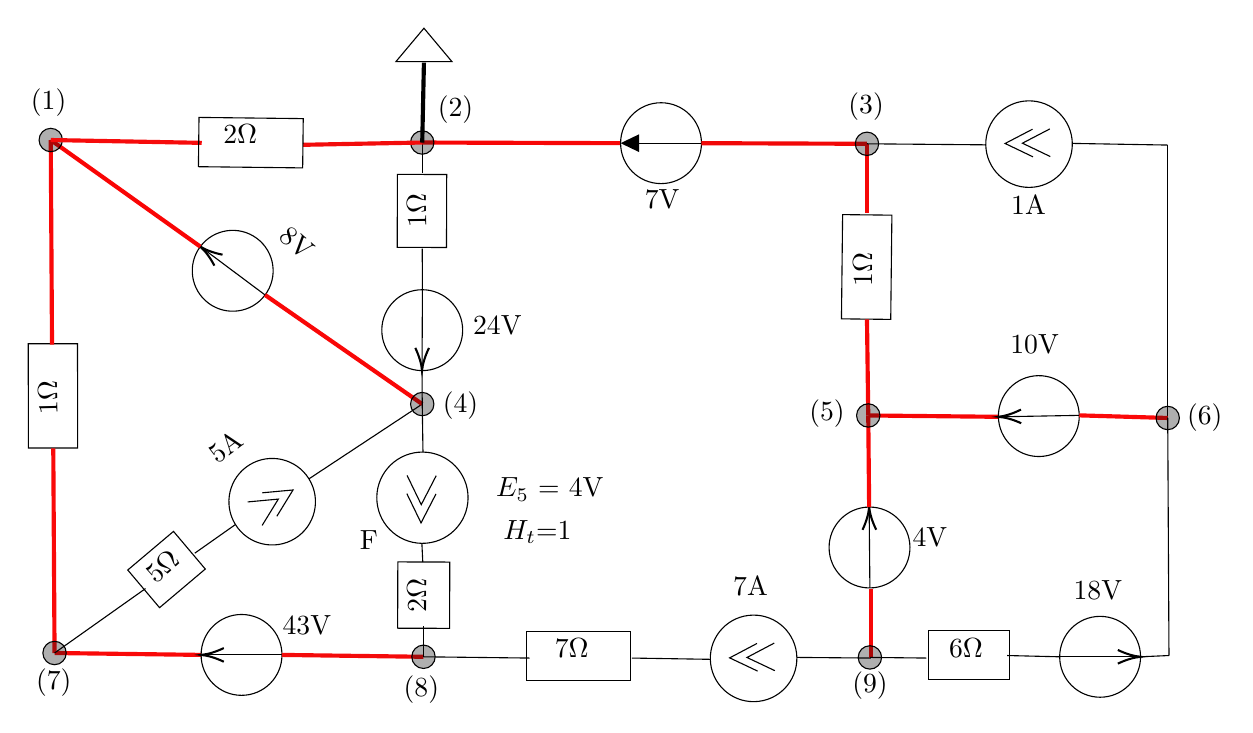
\begin{tikzpicture}[x=0.75pt,y=0.75pt,yscale=-1,xscale=1]
%uncomment if require: \path (0,441); %set diagram left start at 0, and has height of 441

%Flowchart: Connector [id:dp9270801755221227] 
\draw   (542.23,339.34) .. controls (542.23,328.58) and (550.95,319.86) .. (561.71,319.86) .. controls (572.47,319.86) and (581.19,328.58) .. (581.19,339.34) .. controls (581.19,350.1) and (572.47,358.82) .. (561.71,358.82) .. controls (550.95,358.82) and (542.23,350.1) .. (542.23,339.34) -- cycle ;
%Straight Lines [id:da6781562055832304] 
\draw    (542.23,339.34) -- (579.19,339.34) ;
\draw [shift={(581.19,339.34)}, rotate = 180] [color={rgb, 255:red, 0; green, 0; blue, 0 }  ][line width=0.75]    (10.93,-3.29) .. controls (6.95,-1.4) and (3.31,-0.3) .. (0,0) .. controls (3.31,0.3) and (6.95,1.4) .. (10.93,3.29)   ;

%Shape: Rectangle [id:dp4737566977396117] 
\draw   (478.92,326.56) -- (518.18,326.56) -- (518.18,350.3) -- (478.92,350.3) -- cycle ;
%Shape: Rectangle [id:dp9667802879586256] 
\draw   (69.02,188.5) -- (69.11,238.72) -- (45.37,238.76) -- (45.28,188.54) -- cycle ;
%Straight Lines [id:da7347210402357076] 
\draw [color={rgb, 255:red, 249; green, 7; blue, 7 }  ,draw opacity=1 ][line width=1.5]    (56.13,90.36) -- (56.74,188.98) ;
%Straight Lines [id:da30746269499196677] 
\draw [color={rgb, 255:red, 249; green, 10; blue, 10 }  ,draw opacity=1 ][line width=1.5]    (57.35,238.89) -- (57.96,337.51) ;
%Straight Lines [id:da16528068153435105] 
\draw [color={rgb, 255:red, 249; green, 9; blue, 9 }  ,draw opacity=1 ][line width=1.5]    (57.96,337.51) -- (128.57,338.43) ;
%Flowchart: Connector [id:dp40061918108006433] 
\draw   (167.53,338.43) .. controls (167.53,349.19) and (158.81,357.91) .. (148.05,357.91) .. controls (137.3,357.91) and (128.57,349.19) .. (128.57,338.43) .. controls (128.57,327.67) and (137.3,318.95) .. (148.05,318.95) .. controls (158.81,318.95) and (167.53,327.67) .. (167.53,338.43) -- cycle ;
%Straight Lines [id:da4449167399874583] 
\draw    (167.53,338.43) -- (130.57,338.43) ;
\draw [shift={(128.57,338.43)}, rotate = 360] [color={rgb, 255:red, 0; green, 0; blue, 0 }  ][line width=0.75]    (10.93,-3.29) .. controls (6.95,-1.4) and (3.31,-0.3) .. (0,0) .. controls (3.31,0.3) and (6.95,1.4) .. (10.93,3.29)   ;

%Straight Lines [id:da5423321266401198] 
\draw [color={rgb, 255:red, 244; green, 11; blue, 11 }  ,draw opacity=1 ][line width=1.5]    (235.72,339.34) -- (167.53,338.43) ;
%Straight Lines [id:da1333229254706947] 
\draw    (235.11,91.57) -- (235.11,106.18) ;
%Shape: Rectangle [id:dp8147511147447091] 
\draw   (246.9,106.98) -- (246.8,142.14) -- (223.06,142.07) -- (223.15,106.91) -- cycle ;
%Straight Lines [id:da3752772298769764] 
\draw    (235.11,142.71) -- (235.21,162.49) ;
%Flowchart: Connector [id:dp9800044826411813] 
\draw   (235.21,162.49) .. controls (245.96,162.55) and (254.64,171.31) .. (254.59,182.07) .. controls (254.53,192.83) and (245.77,201.51) .. (235.01,201.46) .. controls (224.25,201.4) and (215.57,192.63) .. (215.63,181.88) .. controls (215.68,171.12) and (224.45,162.44) .. (235.21,162.49) -- cycle ;
%Straight Lines [id:da15518000296251477] 
\draw    (235.21,162.49) -- (235.02,199.46) ;
\draw [shift={(235.01,201.46)}, rotate = 270.29] [color={rgb, 255:red, 0; green, 0; blue, 0 }  ][line width=0.75]    (10.93,-3.29) .. controls (6.95,-1.4) and (3.31,-0.3) .. (0,0) .. controls (3.31,0.3) and (6.95,1.4) .. (10.93,3.29)   ;

%Shape: Rectangle [id:dp4139885664271359] 
\draw   (93.23,297.53) -- (115.27,278.92) -- (130.59,297.06) -- (108.55,315.67) -- cycle ;
%Flowchart: Connector [id:dp8841244253872094] 
\draw   (145.11,275.62) .. controls (139.03,265.84) and (142.03,252.98) .. (151.81,246.91) .. controls (161.59,240.83) and (174.45,243.83) .. (180.53,253.61) .. controls (186.6,263.39) and (183.6,276.25) .. (173.82,282.32) .. controls (164.04,288.4) and (151.19,285.4) .. (145.11,275.62) -- cycle ;
\draw   (150.97,264.73) -- (165.78,263.36) -- (157.99,276.03) ;
\draw   (158.05,260.33) -- (172.86,258.96) -- (165.07,271.63) ;

%Straight Lines [id:da6498485089903523] 
\draw    (57.96,337.51) -- (101.79,306.47) ;
%Straight Lines [id:da1648330757903893] 
\draw    (145.11,275.62) -- (125.53,289.42) ;
%Straight Lines [id:da25570294871250665] 
\draw    (235.11,217.59) -- (180.53,253.61) ;
%Flowchart: Connector [id:dp5578065010047788] 
\draw   (159.4,165.02) .. controls (152.96,173.64) and (140.76,175.41) .. (132.14,168.97) .. controls (123.52,162.53) and (121.75,150.33) .. (128.18,141.71) .. controls (134.62,133.09) and (146.83,131.32) .. (155.45,137.75) .. controls (164.07,144.19) and (165.84,156.4) .. (159.4,165.02) -- cycle ;
%Straight Lines [id:da23421547181746738] 
\draw    (159.4,165.02) -- (129.79,142.9) ;
\draw [shift={(128.18,141.71)}, rotate = 36.75] [color={rgb, 255:red, 0; green, 0; blue, 0 }  ][line width=0.75]    (10.93,-3.29) .. controls (6.95,-1.4) and (3.31,-0.3) .. (0,0) .. controls (3.31,0.3) and (6.95,1.4) .. (10.93,3.29)   ;

%Straight Lines [id:da3360778513474214] 
\draw [color={rgb, 255:red, 249; green, 5; blue, 5 }  ,draw opacity=1 ][line width=1.5]    (56.13,90.36) -- (128.18,141.71) ;
%Straight Lines [id:da1355482709182445] 
\draw [color={rgb, 255:red, 249; green, 7; blue, 7 }  ,draw opacity=1 ][line width=1.5]    (159.4,165.02) -- (235.11,217.59) ;
%Straight Lines [id:da10802524495699561] 
\draw [color={rgb, 255:red, 247; green, 6; blue, 6 }  ,draw opacity=1 ][line width=1.5]    (235.11,91.57) -- (330.68,91.88) ;
%Flowchart: Connector [id:dp5057766104260943] 
\draw   (330.68,91.88) .. controls (330.68,81.12) and (339.4,72.4) .. (350.16,72.4) .. controls (360.92,72.4) and (369.64,81.12) .. (369.64,91.88) .. controls (369.64,102.64) and (360.92,111.36) .. (350.16,111.36) .. controls (339.4,111.36) and (330.68,102.64) .. (330.68,91.88) -- cycle ;
%Straight Lines [id:da3181224817766224] 
\draw    (333.68,91.88) -- (369.64,91.88) ;
\draw [shift={(330.68,91.88)}, rotate = 0] [fill={rgb, 255:red, 0; green, 0; blue, 0 }  ][line width=0.08]  [draw opacity=0] (8.93,-4.29) -- (0,0) -- (8.93,4.29) -- cycle    ;
%Straight Lines [id:da5180293715512814] 
\draw [color={rgb, 255:red, 241; green, 8; blue, 8 }  ,draw opacity=1 ][line width=1.5]    (369.64,91.88) -- (449.39,92.18) ;
%Straight Lines [id:da6785576903938952] 
\draw    (286.85,339.95) -- (235.72,339.34) ;
%Shape: Rectangle [id:dp43490317766124353] 
\draw   (285.33,327.17) -- (335.55,327.17) -- (335.55,350.91) -- (285.33,350.91) -- cycle ;
%Straight Lines [id:da06229672444698431] 
\draw    (373.91,340.56) -- (336.16,339.95) ;
%Flowchart: Connector [id:dp7851498713964808] 
\draw   (415.6,339.64) .. controls (415.85,351.16) and (406.73,360.69) .. (395.21,360.95) .. controls (383.7,361.2) and (374.16,352.07) .. (373.91,340.56) .. controls (373.66,329.05) and (382.78,319.51) .. (394.3,319.26) .. controls (405.81,319) and (415.35,328.13) .. (415.6,339.64) -- cycle ;
\draw   (405.02,346.03) -- (391.57,339.67) -- (404.72,332.73) ;
\draw   (396.68,346.22) -- (383.23,339.86) -- (396.39,332.92) ;

%Straight Lines [id:da9185246580674729] 
\draw    (451.22,339.95) -- (415.6,339.64) ;
%Straight Lines [id:da750326464081535] 
\draw [color={rgb, 255:red, 247; green, 7; blue, 7 }  ,draw opacity=1 ][line width=1.5]    (451.22,306.47) -- (451.22,339.95) ;
%Flowchart: Connector [id:dp2681269475222585] 
\draw   (450.79,306.16) .. controls (440.03,306.26) and (431.23,297.62) .. (431.13,286.86) .. controls (431.03,276.1) and (439.67,267.3) .. (450.43,267.2) .. controls (461.19,267.1) and (469.99,275.74) .. (470.09,286.5) .. controls (470.19,297.26) and (461.55,306.06) .. (450.79,306.16) -- cycle ;
%Straight Lines [id:da46089558980747936] 
\draw    (450.79,306.16) -- (450.45,269.2) ;
\draw [shift={(450.43,267.2)}, rotate = 89.47] [color={rgb, 255:red, 0; green, 0; blue, 0 }  ][line width=0.75]    (10.93,-3.29) .. controls (6.95,-1.4) and (3.31,-0.3) .. (0,0) .. controls (3.31,0.3) and (6.95,1.4) .. (10.93,3.29)   ;

%Straight Lines [id:da2321409034543207] 
\draw [color={rgb, 255:red, 249; green, 6; blue, 6 }  ,draw opacity=1 ][line width=1.5]    (450,223.07) -- (450.43,267.2) ;
%Straight Lines [id:da8769965982394923] 
\draw [color={rgb, 255:red, 246; green, 7; blue, 7 }  ,draw opacity=1 ][line width=1.5]    (449.39,92.18) -- (449.39,125.66) ;
%Shape: Rectangle [id:dp4867788140885223] 
\draw   (461.39,126.56) -- (460.83,176.78) -- (437.09,176.52) -- (437.65,126.3) -- cycle ;
%Straight Lines [id:da7875812451856252] 
\draw [color={rgb, 255:red, 247; green, 6; blue, 6 }  ,draw opacity=1 ][line width=1.5]    (450,223.07) -- (449.39,176.8) ;
%Straight Lines [id:da6536587562096758] 
\draw    (449.39,92.18) -- (506.62,92.68) ;
%Flowchart: Connector [id:dp17553917091137916] 
\draw   (548.31,91.99) .. controls (548.5,103.5) and (539.33,112.99) .. (527.81,113.18) .. controls (516.3,113.37) and (506.81,104.19) .. (506.62,92.68) .. controls (506.43,81.17) and (515.61,71.68) .. (527.12,71.49) .. controls (538.63,71.3) and (548.12,80.48) .. (548.31,91.99) -- cycle ;
\draw   (537.69,98.32) -- (524.28,91.89) -- (537.47,85.02) ;
\draw   (529.36,98.46) -- (515.94,92.03) -- (529.13,85.16) ;

%Straight Lines [id:da18482728121268854] 
\draw    (548.31,91.99) -- (594.28,92.79) ;
%Straight Lines [id:da7498258113423346] 
\draw    (594.28,92.79) -- (594.28,224.28) ;
%Straight Lines [id:da940259620577877] 
\draw [color={rgb, 255:red, 247; green, 6; blue, 6 }  ,draw opacity=1 ][line width=1.5]    (512.71,223.72) -- (450,223.07) ;
%Flowchart: Connector [id:dp6624088763704992] 
\draw   (551.66,223.02) .. controls (551.86,233.77) and (543.29,242.65) .. (532.54,242.85) .. controls (521.78,243.04) and (512.9,234.48) .. (512.71,223.72) .. controls (512.51,212.97) and (521.07,204.09) .. (531.83,203.89) .. controls (542.59,203.7) and (551.47,212.26) .. (551.66,223.02) -- cycle ;
%Straight Lines [id:da5732322951082511] 
\draw    (551.66,223.02) -- (514.71,223.69) ;
\draw [shift={(512.71,223.72)}, rotate = 358.96] [color={rgb, 255:red, 0; green, 0; blue, 0 }  ][line width=0.75]    (10.93,-3.29) .. controls (6.95,-1.4) and (3.31,-0.3) .. (0,0) .. controls (3.31,0.3) and (6.95,1.4) .. (10.93,3.29)   ;

%Straight Lines [id:da7773054828023371] 
\draw [color={rgb, 255:red, 251; green, 9; blue, 9 }  ,draw opacity=1 ][line width=1.5]    (551.66,223.02) -- (594.28,224.28) ;
%Straight Lines [id:da9651126430027448] 
\draw    (450.79,339.64) -- (478,339.95) ;
%Straight Lines [id:da23967528935399973] 
\draw    (542.23,339.34) -- (516.96,338.73) ;
%Straight Lines [id:da9296553319859571] 
\draw    (594.28,224.28) -- (594.89,338.73) ;
%Straight Lines [id:da38754316585407866] 
\draw    (581.19,339.34) -- (594.89,338.73) ;
%Shape: Ellipse [id:dp7882674071011084] 
\draw  [fill={rgb, 255:red, 13; green, 12; blue, 12 }  ,fill opacity=0.33 ] (50.5,90.36) .. controls (50.5,87.25) and (53.02,84.72) .. (56.13,84.72) .. controls (59.24,84.72) and (61.76,87.25) .. (61.76,90.36) .. controls (61.76,93.47) and (59.24,95.99) .. (56.13,95.99) .. controls (53.02,95.99) and (50.5,93.47) .. (50.5,90.36) -- cycle ;
%Shape: Ellipse [id:dp7538292901722516] 
\draw  [fill={rgb, 255:red, 13; green, 12; blue, 12 }  ,fill opacity=0.33 ] (229.48,91.57) .. controls (229.48,88.46) and (232,85.94) .. (235.11,85.94) .. controls (238.22,85.94) and (240.74,88.46) .. (240.74,91.57) .. controls (240.74,94.68) and (238.22,97.2) .. (235.11,97.2) .. controls (232,97.2) and (229.48,94.68) .. (229.48,91.57) -- cycle ;
%Shape: Ellipse [id:dp24657752652752118] 
\draw  [fill={rgb, 255:red, 13; green, 12; blue, 12 }  ,fill opacity=0.33 ] (229.48,217.59) .. controls (229.48,214.48) and (232,211.96) .. (235.11,211.96) .. controls (238.22,211.96) and (240.74,214.48) .. (240.74,217.59) .. controls (240.74,220.7) and (238.22,223.22) .. (235.11,223.22) .. controls (232,223.22) and (229.48,220.7) .. (229.48,217.59) -- cycle ;
%Shape: Ellipse [id:dp8023182388888381] 
\draw  [fill={rgb, 255:red, 13; green, 12; blue, 12 }  ,fill opacity=0.33 ] (52.33,337.51) .. controls (52.33,334.4) and (54.85,331.88) .. (57.96,331.88) .. controls (61.07,331.88) and (63.59,334.4) .. (63.59,337.51) .. controls (63.59,340.62) and (61.07,343.15) .. (57.96,343.15) .. controls (54.85,343.15) and (52.33,340.62) .. (52.33,337.51) -- cycle ;
%Shape: Ellipse [id:dp9965555730253974] 
\draw  [fill={rgb, 255:red, 13; green, 12; blue, 12 }  ,fill opacity=0.33 ] (230.08,339.34) .. controls (230.08,336.23) and (232.61,333.71) .. (235.72,333.71) .. controls (238.83,333.71) and (241.35,336.23) .. (241.35,339.34) .. controls (241.35,342.45) and (238.83,344.97) .. (235.72,344.97) .. controls (232.61,344.97) and (230.08,342.45) .. (230.08,339.34) -- cycle ;
%Shape: Ellipse [id:dp4863208895647082] 
\draw  [fill={rgb, 255:red, 13; green, 12; blue, 12 }  ,fill opacity=0.33 ] (443.76,92.18) .. controls (443.76,89.07) and (446.28,86.55) .. (449.39,86.55) .. controls (452.5,86.55) and (455.02,89.07) .. (455.02,92.18) .. controls (455.02,95.29) and (452.5,97.81) .. (449.39,97.81) .. controls (446.28,97.81) and (443.76,95.29) .. (443.76,92.18) -- cycle ;
%Shape: Ellipse [id:dp14045591679570468] 
\draw  [fill={rgb, 255:red, 13; green, 12; blue, 12 }  ,fill opacity=0.33 ] (444.37,223.07) .. controls (444.37,219.96) and (446.89,217.44) .. (450,217.44) .. controls (453.11,217.44) and (455.63,219.96) .. (455.63,223.07) .. controls (455.63,226.18) and (453.11,228.7) .. (450,228.7) .. controls (446.89,228.7) and (444.37,226.18) .. (444.37,223.07) -- cycle ;
%Shape: Ellipse [id:dp15823477089237037] 
\draw  [fill={rgb, 255:red, 13; green, 12; blue, 12 }  ,fill opacity=0.33 ] (445.16,339.64) .. controls (445.16,336.53) and (447.68,334.01) .. (450.79,334.01) .. controls (453.9,334.01) and (456.42,336.53) .. (456.42,339.64) .. controls (456.42,342.75) and (453.9,345.28) .. (450.79,345.28) .. controls (447.68,345.28) and (445.16,342.75) .. (445.16,339.64) -- cycle ;
%Shape: Ellipse [id:dp677101212612778] 
\draw  [fill={rgb, 255:red, 13; green, 12; blue, 12 }  ,fill opacity=0.33 ] (588.65,224.28) .. controls (588.65,221.17) and (591.17,218.65) .. (594.28,218.65) .. controls (597.39,218.65) and (599.91,221.17) .. (599.91,224.28) .. controls (599.91,227.39) and (597.39,229.92) .. (594.28,229.92) .. controls (591.17,229.92) and (588.65,227.39) .. (588.65,224.28) -- cycle ;
%Straight Lines [id:da9969100544045801] 
\draw [color={rgb, 255:red, 246; green, 11; blue, 11 }  ,draw opacity=1 ][line width=1.5]    (56.13,90.36) -- (128.88,91.73) ;
%Straight Lines [id:da4534443226215574] 
\draw [color={rgb, 255:red, 242; green, 12; blue, 12 }  ,draw opacity=1 ][line width=1.5]    (177.67,92.67) -- (235.11,91.57) ;
%Shape: Triangle [id:dp23800541797803199] 
\draw   (235.93,36.5) -- (249.4,52.56) -- (222.46,52.56) -- cycle ;
%Straight Lines [id:da1106051011867617] 
\draw [line width=1.5]    (235.11,91.57) -- (235.93,53.08) ;
%Straight Lines [id:da5000513881542927] 
\draw    (235.72,324.58) -- (235.72,339.34) ;
%Shape: Rectangle [id:dp4053091123845911] 
\draw   (248.38,293.7) -- (248.29,325.63) -- (223.26,325.56) -- (223.35,293.63) -- cycle ;
%Flowchart: Connector [id:dp9687617106423128] 
\draw   (235.47,240.71) .. controls (247.61,240.86) and (257.34,250.82) .. (257.19,262.96) .. controls (257.04,275.1) and (247.08,284.82) .. (234.94,284.68) .. controls (222.8,284.53) and (213.08,274.57) .. (213.22,262.43) .. controls (213.37,250.29) and (223.33,240.56) .. (235.47,240.71) -- cycle ;
\draw   (241.83,252.09) -- (234.64,266.04) -- (227.8,251.93) ;
\draw   (241.72,260.89) -- (234.54,274.83) -- (227.69,260.72) ;

%Straight Lines [id:da7119558174131766] 
\draw    (235.37,293.66) -- (234.94,284.68) ;
%Straight Lines [id:da6354349017561942] 
\draw    (235.47,240.71) -- (235.11,217.59) ;
%Straight Lines [id:da29081232384814926] 
\draw    (235.01,201.46) -- (235.11,217.59) ;
%Shape: Rectangle [id:dp22581493636674388] 
\draw   (127.56,79.47) -- (177.78,80.05) -- (177.5,103.79) -- (127.28,103.21) -- cycle ;

% Text Node
\draw (129.17,239.22) node [anchor=north west][inner sep=0.75pt]  [rotate=-322.88] [align=left] {5A};
% Text Node
\draw (166.58,318.21) node [anchor=north west][inner sep=0.75pt]   [align=left] {43V};
% Text Node
\draw (171.35,128.97) node [anchor=north west][inner sep=0.75pt]  [rotate=-41.03] [align=left] {8V};
% Text Node
\draw (258.35,173.63) node [anchor=north west][inner sep=0.75pt]   [align=left] {24V};
% Text Node
\draw (341.08,112.75) node [anchor=north west][inner sep=0.75pt]   [align=left] {7V};
% Text Node
\draw (383.69,299.64) node [anchor=north west][inner sep=0.75pt]   [align=left] {7A};
% Text Node
\draw (470.13,275.9) node [anchor=north west][inner sep=0.75pt]   [align=left] {4V};
% Text Node
\draw (547.67,301.47) node [anchor=north west][inner sep=0.75pt]   [align=left] {18V};
% Text Node
\draw (517.23,183.06) node [anchor=north west][inner sep=0.75pt]   [align=left] {10V};
% Text Node
\draw (517.62,116.1) node [anchor=north west][inner sep=0.75pt]   [align=left] {1A};
% Text Node
\draw (49.09,224.05) node [anchor=north west][inner sep=0.75pt]  [rotate=-268.74] [align=left] {1\ohm};
% Text Node
\draw (98.88,297.54) node [anchor=north west][inner sep=0.75pt]  [rotate=-318.32] [align=left] {5\ohm};
% Text Node
\draw (226.73,133.87) node [anchor=north west][inner sep=0.75pt]  [rotate=-269.34] [align=left] {1\ohm};
% Text Node
\draw (297.77,329.47) node [anchor=north west][inner sep=0.75pt]   [align=left] {7\ohm};
% Text Node
\draw (441.48,162.07) node [anchor=north west][inner sep=0.75pt]  [rotate=-270.09] [align=left] {1\ohm};
% Text Node
\draw (487.7,329.17) node [anchor=north west][inner sep=0.75pt]   [align=left] {6\ohm};
% Text Node
\draw (45.33,64.35) node [anchor=north west][inner sep=0.75pt]   [align=left] {(1)};
% Text Node
\draw (241.35,67.7) node [anchor=north west][inner sep=0.75pt]   [align=left] {(2)};
% Text Node
\draw (439.2,66.18) node [anchor=north west][inner sep=0.75pt]   [align=left] {(3)};
% Text Node
\draw (243.79,210.46) node [anchor=north west][inner sep=0.75pt]   [align=left] {(4)};
% Text Node
\draw (420.33,214.11) node [anchor=north west][inner sep=0.75pt]   [align=left] {(5)};
% Text Node
\draw (602.35,215.94) node [anchor=north west][inner sep=0.75pt]   [align=left] {(6)};
% Text Node
\draw (47.76,343.78) node [anchor=north west][inner sep=0.75pt]   [align=left] {(7)};
% Text Node
\draw (224.91,347.12) node [anchor=north west][inner sep=0.75pt]   [align=left] {(8)};
% Text Node
\draw (441.03,345.3) node [anchor=north west][inner sep=0.75pt]   [align=left] {(9)};
% Text Node
\draw (226.58,319.1) node [anchor=north west][inner sep=0.75pt]  [rotate=-270.58] [align=left] {2\ohm};
% Text Node
\draw (203.75,277.17) node [anchor=north west][inner sep=0.75pt]   [align=left] {F};
% Text Node
\draw (269.42,251.93) node [anchor=north west][inner sep=0.75pt]   [align=left] {$\displaystyle E_{5}$ = 4V};
% Text Node
\draw (272.88,272.47) node [anchor=north west][inner sep=0.75pt]   [align=left] {$\displaystyle H_{t}$=1};
% Text Node
\draw (138,81.67) node [anchor=north west][inner sep=0.75pt]   [align=left] {$\displaystyle 2\si{\ohm}$};


\end{tikzpicture}

\end{center}

\newpage

În circuitul de mai sus am ales ca pe latura dintre nodul \textbf{(4)} și \textbf{(8)} să plasăm sursa de curent comandată. Cu ajutorul \emph{LTSpice-ului} și \emph{netlist-ului} am identificat orientarea intensității și astfel am orientat și sursa de curent comandată. Ca post de latură de transfer am ales latura dintre nod-ul \textbf{(5)} și \textbf{(9)}, care deja are un \emph{SIT} deci nu va fi nevoie pentru LTSpice să definim un \emph{SIT} de valoare \textbf{0}. Dacă rulăm circuitul cu operatorul \textbf{.op} vom afla că $I_{p1} = 11A$ și $I_{p2} = 11A$, de unde rezultă din formula de calcul a factorului de transfer că valoarea acestuia este $H_t = 1$. După ce am făcut toate calculele de vigoare vom rula circuitul cu operatorul \textbf{.op} ca să comparăm datele de ieșire \emph{inițiale} cu datele de ieșire după ce am adăugat un \textbf{SICI}.


\begin{figure}[h]
    \centering
    \includegraphics[width=\linewidth, height=\textheight, keepaspectratio]{Compar_data.png}
    \caption{Datele înainte și după adăugarea unui SICI}
    \label{fig:SICI}
\end{figure}

După cum putem observa datele nu s-au modificat ceea ce rezultă că adăugarea sursei de curent comandate a fost efectuată cu success!
\newpage

\section{Rezolvarea circuitelor de curent alternativ}
Pentru această secțiune vom adăuga la circuitul nostru din secțiunea 1, o bobină în serie cu o rezistență pozitivă și un condensator în paralel la fel cu o rezistență pozitivă, cu valorile specificate în enunțul temei. Deci circuitul se transformă în următoarea schemă:

\hspace{-3cm}
\begin{center}
    

\tikzset{every picture/.style={line width=0.75pt}} %set default line width to 0.75pt        

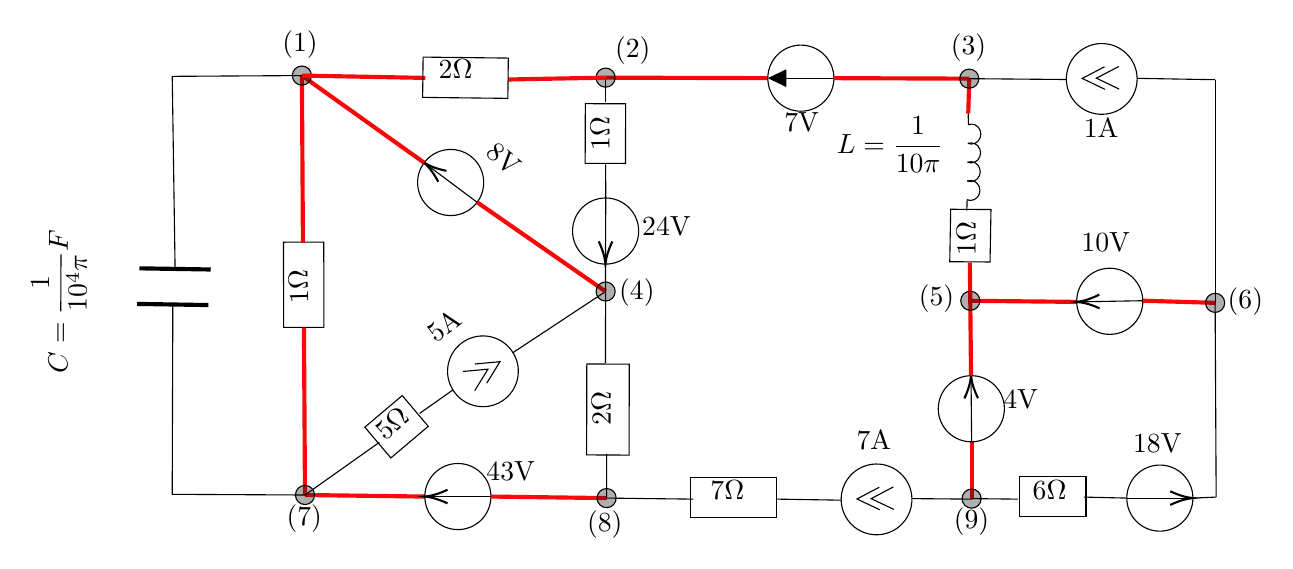
\begin{tikzpicture}[x=0.75pt,y=0.75pt,yscale=-1,xscale=1]
%uncomment if require: \path (0,441); %set diagram left start at 0, and has height of 441

%Flowchart: Connector [id:dp9270801755221227] 
\draw   (537.15,243.74) .. controls (537.15,234.95) and (544.28,227.82) .. (553.08,227.82) .. controls (561.87,227.82) and (569,234.95) .. (569,243.74) .. controls (569,252.54) and (561.87,259.67) .. (553.08,259.67) .. controls (544.28,259.67) and (537.15,252.54) .. (537.15,243.74) -- cycle ;
%Straight Lines [id:da6781562055832304] 
\draw    (537.15,243.74) -- (567,243.74) ;
\draw [shift={(569,243.74)}, rotate = 180] [color={rgb, 255:red, 0; green, 0; blue, 0 }  ][line width=0.75]    (10.93,-3.29) .. controls (6.95,-1.4) and (3.31,-0.3) .. (0,0) .. controls (3.31,0.3) and (6.95,1.4) .. (10.93,3.29)   ;

%Shape: Rectangle [id:dp9293540676010876] 
\draw   (485.39,233.29) -- (517.49,233.29) -- (517.49,252.7) -- (485.39,252.7) -- cycle ;
%Shape: Rectangle [id:dp29329609290946057] 
\draw   (150.25,120.41) -- (150.32,161.48) -- (130.91,161.51) -- (130.84,120.45) -- cycle ;
%Straight Lines [id:da9200519684082165] 
\draw [color={rgb, 255:red, 249; green, 7; blue, 7 }  ,draw opacity=1 ][line width=1.5]    (139.71,40.17) -- (140.21,120.8) ;
%Straight Lines [id:da7448029658822661] 
\draw [color={rgb, 255:red, 249; green, 10; blue, 10 }  ,draw opacity=1 ][line width=1.5]    (140.7,161.62) -- (141.2,242.25) ;
%Straight Lines [id:da6489888369249426] 
\draw [color={rgb, 255:red, 249; green, 9; blue, 9 }  ,draw opacity=1 ][line width=1.5]    (141.2,242.25) -- (198.94,243) ;
%Flowchart: Connector [id:dp40061918108006433] 
\draw   (230.79,243) .. controls (230.79,251.79) and (223.66,258.92) .. (214.87,258.92) .. controls (206.07,258.92) and (198.94,251.79) .. (198.94,243) .. controls (198.94,234.2) and (206.07,227.07) .. (214.87,227.07) .. controls (223.66,227.07) and (230.79,234.2) .. (230.79,243) -- cycle ;
%Straight Lines [id:da4449167399874583] 
\draw    (230.79,243) -- (200.94,243) ;
\draw [shift={(198.94,243)}, rotate = 360] [color={rgb, 255:red, 0; green, 0; blue, 0 }  ][line width=0.75]    (10.93,-3.29) .. controls (6.95,-1.4) and (3.31,-0.3) .. (0,0) .. controls (3.31,0.3) and (6.95,1.4) .. (10.93,3.29)   ;

%Straight Lines [id:da09666830991124842] 
\draw [color={rgb, 255:red, 244; green, 11; blue, 11 }  ,draw opacity=1 ][line width=1.5]    (286.54,243.74) -- (230.79,243) ;
%Straight Lines [id:da6051461333969024] 
\draw    (286.04,41.17) -- (286.04,53.11) ;
%Shape: Rectangle [id:dp8337970185791892] 
\draw   (295.68,53.76) -- (295.6,82.51) -- (276.19,82.46) -- (276.27,53.71) -- cycle ;
%Straight Lines [id:da41632975873257627] 
\draw    (286.04,82.97) -- (286.12,99.15) ;
%Flowchart: Connector [id:dp9800044826411813] 
\draw   (286.12,99.15) .. controls (294.92,99.2) and (302.01,106.36) .. (301.97,115.16) .. controls (301.93,123.96) and (294.76,131.05) .. (285.96,131.01) .. controls (277.17,130.96) and (270.07,123.79) .. (270.12,115) .. controls (270.16,106.2) and (277.33,99.11) .. (286.12,99.15) -- cycle ;
%Straight Lines [id:da15518000296251477] 
\draw    (286.12,99.15) -- (285.97,129.01) ;
\draw [shift={(285.96,131.01)}, rotate = 270.29] [color={rgb, 255:red, 0; green, 0; blue, 0 }  ][line width=0.75]    (10.93,-3.29) .. controls (6.95,-1.4) and (3.31,-0.3) .. (0,0) .. controls (3.31,0.3) and (6.95,1.4) .. (10.93,3.29)   ;

%Shape: Rectangle [id:dp5767279698085399] 
\draw   (170.04,209.56) -- (188.06,194.34) -- (200.58,209.17) -- (182.57,224.39) -- cycle ;
%Flowchart: Connector [id:dp8841244253872094] 
\draw   (212.46,191.64) .. controls (207.49,183.65) and (209.94,173.14) .. (217.94,168.17) .. controls (225.94,163.2) and (236.45,165.65) .. (241.42,173.65) .. controls (246.39,181.64) and (243.93,192.16) .. (235.94,197.13) .. controls (227.94,202.09) and (217.43,199.64) .. (212.46,191.64) -- cycle ;
\draw   (217.25,182.74) -- (229.36,181.62) -- (222.99,191.98) ;
\draw   (223.04,179.14) -- (235.15,178.02) -- (228.78,188.38) ;

%Straight Lines [id:da553190898070141] 
\draw    (141.2,242.25) -- (177.04,216.87) ;
%Straight Lines [id:da08358419736444067] 
\draw    (212.46,191.64) -- (196.45,202.93) ;
%Straight Lines [id:da6192014247564932] 
\draw    (286.04,144.2) -- (241.42,173.65) ;
%Flowchart: Connector [id:dp5578065010047788] 
\draw   (224.14,101.21) .. controls (218.88,108.26) and (208.9,109.71) .. (201.85,104.45) .. controls (194.8,99.18) and (193.36,89.2) .. (198.62,82.16) .. controls (203.88,75.11) and (213.86,73.66) .. (220.91,78.92) .. controls (227.96,84.19) and (229.41,94.17) .. (224.14,101.21) -- cycle ;
%Straight Lines [id:da23421547181746738] 
\draw    (224.14,101.21) -- (200.22,83.35) ;
\draw [shift={(198.62,82.16)}, rotate = 36.75] [color={rgb, 255:red, 0; green, 0; blue, 0 }  ][line width=0.75]    (10.93,-3.29) .. controls (6.95,-1.4) and (3.31,-0.3) .. (0,0) .. controls (3.31,0.3) and (6.95,1.4) .. (10.93,3.29)   ;

%Straight Lines [id:da9086515311629166] 
\draw [color={rgb, 255:red, 249; green, 5; blue, 5 }  ,draw opacity=1 ][line width=1.5]    (139.71,40.17) -- (198.62,82.16) ;
%Straight Lines [id:da35276082352041604] 
\draw [color={rgb, 255:red, 249; green, 7; blue, 7 }  ,draw opacity=1 ][line width=1.5]    (224.14,101.21) -- (286.04,144.2) ;
%Straight Lines [id:da252532111241782] 
\draw [color={rgb, 255:red, 247; green, 6; blue, 6 }  ,draw opacity=1 ][line width=1.5]    (286.04,41.17) -- (364.19,41.41) ;
%Flowchart: Connector [id:dp7804241321682361] 
\draw   (364.19,41.41) .. controls (364.19,32.62) and (371.32,25.49) .. (380.11,25.49) .. controls (388.91,25.49) and (396.04,32.62) .. (396.04,41.41) .. controls (396.04,50.21) and (388.91,57.34) .. (380.11,57.34) .. controls (371.32,57.34) and (364.19,50.21) .. (364.19,41.41) -- cycle ;
%Straight Lines [id:da36901245690350337] 
\draw    (367.19,41.41) -- (396.04,41.41) ;
\draw [shift={(364.19,41.41)}, rotate = 0] [fill={rgb, 255:red, 0; green, 0; blue, 0 }  ][line width=0.08]  [draw opacity=0] (8.93,-4.29) -- (0,0) -- (8.93,4.29) -- cycle    ;
%Straight Lines [id:da537630088678422] 
\draw [color={rgb, 255:red, 241; green, 8; blue, 8 }  ,draw opacity=1 ][line width=1.5]    (396.04,41.41) -- (461.25,41.66) ;
%Straight Lines [id:da9906748730155359] 
\draw    (328.35,244.24) -- (286.54,243.74) ;
%Shape: Rectangle [id:dp6048901001428784] 
\draw   (327.11,233.79) -- (368.17,233.79) -- (368.17,253.2) -- (327.11,253.2) -- cycle ;
%Straight Lines [id:da05140142628507394] 
\draw    (399.53,244.74) -- (368.67,244.24) ;
%Flowchart: Connector [id:dp7851498713964808] 
\draw   (433.62,243.99) .. controls (433.82,253.4) and (426.36,261.2) .. (416.95,261.41) .. controls (407.54,261.62) and (399.74,254.15) .. (399.53,244.74) .. controls (399.32,235.33) and (406.79,227.53) .. (416.2,227.32) .. controls (425.61,227.11) and (433.41,234.58) .. (433.62,243.99) -- cycle ;
\draw   (424.96,249.21) -- (413.97,244.02) -- (424.72,238.34) ;
\draw   (418.15,249.36) -- (407.15,244.17) -- (417.91,238.49) ;

%Straight Lines [id:da47951794810794235] 
\draw    (462.74,244.24) -- (433.62,243.99) ;
%Straight Lines [id:da8903781132479665] 
\draw [color={rgb, 255:red, 247; green, 7; blue, 7 }  ,draw opacity=1 ][line width=1.5]    (462.74,216.87) -- (462.74,244.24) ;
%Flowchart: Connector [id:dp2681269475222585] 
\draw   (462.39,216.62) .. controls (453.59,216.7) and (446.4,209.63) .. (446.31,200.84) .. controls (446.23,192.04) and (453.3,184.84) .. (462.09,184.76) .. controls (470.89,184.68) and (478.09,191.75) .. (478.17,200.54) .. controls (478.25,209.34) and (471.18,216.53) .. (462.39,216.62) -- cycle ;
%Straight Lines [id:da46089558980747936] 
\draw    (462.39,216.62) -- (462.11,186.76) ;
\draw [shift={(462.09,184.76)}, rotate = 89.47] [color={rgb, 255:red, 0; green, 0; blue, 0 }  ][line width=0.75]    (10.93,-3.29) .. controls (6.95,-1.4) and (3.31,-0.3) .. (0,0) .. controls (3.31,0.3) and (6.95,1.4) .. (10.93,3.29)   ;

%Straight Lines [id:da8955156878476656] 
\draw [color={rgb, 255:red, 249; green, 6; blue, 6 }  ,draw opacity=1 ][line width=1.5]    (461.74,148.68) -- (462.09,184.76) ;
%Straight Lines [id:da06837581203020537] 
\draw [color={rgb, 255:red, 246; green, 7; blue, 7 }  ,draw opacity=1 ][line width=1.5]    (461.25,41.66) -- (460.76,58.37) ;
%Shape: Rectangle [id:dp6274022256775649] 
\draw   (471.71,104.72) -- (471.26,129.98) -- (451.85,129.85) -- (452.3,104.58) -- cycle ;
%Straight Lines [id:da9778148286536019] 
\draw [color={rgb, 255:red, 247; green, 6; blue, 6 }  ,draw opacity=1 ][line width=1.5]    (461.74,148.68) -- (461.52,130.34) ;
%Straight Lines [id:da09839621372373042] 
\draw    (461.25,41.66) -- (508.03,42.07) ;
%Flowchart: Connector [id:dp17553917091137916] 
\draw   (542.12,41.5) .. controls (542.28,50.92) and (534.78,58.68) .. (525.36,58.83) .. controls (515.95,58.99) and (508.19,51.48) .. (508.03,42.07) .. controls (507.88,32.66) and (515.38,24.9) .. (524.8,24.74) .. controls (534.21,24.59) and (541.97,32.09) .. (542.12,41.5) -- cycle ;
\draw   (533.44,46.68) -- (522.48,41.42) -- (533.26,35.81) ;
\draw   (526.62,46.8) -- (515.66,41.54) -- (526.44,35.92) ;

%Straight Lines [id:da9179241293539009] 
\draw    (542.12,41.5) -- (579.71,42.16) ;
%Straight Lines [id:da45086334447776544] 
\draw    (579.71,42.16) -- (579.71,149.67) ;
%Straight Lines [id:da973646209034035] 
\draw [color={rgb, 255:red, 247; green, 6; blue, 6 }  ,draw opacity=1 ][line width=1.5]    (513.01,149.21) -- (461.74,148.68) ;
%Flowchart: Connector [id:dp6624088763704992] 
\draw   (544.86,148.64) .. controls (545.02,157.43) and (538.02,164.69) .. (529.23,164.85) .. controls (520.43,165.01) and (513.17,158.01) .. (513.01,149.21) .. controls (512.85,140.42) and (519.85,133.16) .. (528.65,133) .. controls (537.44,132.84) and (544.7,139.84) .. (544.86,148.64) -- cycle ;
%Straight Lines [id:da5732322951082511] 
\draw    (544.86,148.64) -- (515.01,149.18) ;
\draw [shift={(513.01,149.21)}, rotate = 358.96] [color={rgb, 255:red, 0; green, 0; blue, 0 }  ][line width=0.75]    (10.93,-3.29) .. controls (6.95,-1.4) and (3.31,-0.3) .. (0,0) .. controls (3.31,0.3) and (6.95,1.4) .. (10.93,3.29)   ;

%Straight Lines [id:da16186527761721337] 
\draw [color={rgb, 255:red, 251; green, 9; blue, 9 }  ,draw opacity=1 ][line width=1.5]    (544.86,148.64) -- (579.71,149.67) ;
%Straight Lines [id:da943222323860289] 
\draw    (462.39,243.99) -- (484.64,244.24) ;
%Straight Lines [id:da3483323460298433] 
\draw    (537.15,243.74) -- (516.49,243.25) ;
%Straight Lines [id:da38661870855581526] 
\draw    (579.71,149.67) -- (580.2,243.25) ;
%Straight Lines [id:da640016388172159] 
\draw    (569,243.74) -- (580.2,243.25) ;
%Shape: Ellipse [id:dp5681357757718268] 
\draw  [fill={rgb, 255:red, 13; green, 12; blue, 12 }  ,fill opacity=0.33 ] (135.1,40.17) .. controls (135.1,37.63) and (137.17,35.57) .. (139.71,35.57) .. controls (142.25,35.57) and (144.31,37.63) .. (144.31,40.17) .. controls (144.31,42.71) and (142.25,44.77) .. (139.71,44.77) .. controls (137.17,44.77) and (135.1,42.71) .. (135.1,40.17) -- cycle ;
%Shape: Ellipse [id:dp710172954664315] 
\draw  [fill={rgb, 255:red, 13; green, 12; blue, 12 }  ,fill opacity=0.33 ] (281.44,41.17) .. controls (281.44,38.62) and (283.5,36.56) .. (286.04,36.56) .. controls (288.59,36.56) and (290.65,38.62) .. (290.65,41.17) .. controls (290.65,43.71) and (288.59,45.77) .. (286.04,45.77) .. controls (283.5,45.77) and (281.44,43.71) .. (281.44,41.17) -- cycle ;
%Shape: Ellipse [id:dp6048704080247278] 
\draw  [fill={rgb, 255:red, 13; green, 12; blue, 12 }  ,fill opacity=0.33 ] (281.44,144.2) .. controls (281.44,141.65) and (283.5,139.59) .. (286.04,139.59) .. controls (288.59,139.59) and (290.65,141.65) .. (290.65,144.2) .. controls (290.65,146.74) and (288.59,148.8) .. (286.04,148.8) .. controls (283.5,148.8) and (281.44,146.74) .. (281.44,144.2) -- cycle ;
%Shape: Ellipse [id:dp2070738198671187] 
\draw  [fill={rgb, 255:red, 13; green, 12; blue, 12 }  ,fill opacity=0.33 ] (136.6,242.25) .. controls (136.6,239.71) and (138.66,237.65) .. (141.2,237.65) .. controls (143.74,237.65) and (145.81,239.71) .. (145.81,242.25) .. controls (145.81,244.79) and (143.74,246.85) .. (141.2,246.85) .. controls (138.66,246.85) and (136.6,244.79) .. (136.6,242.25) -- cycle ;
%Shape: Ellipse [id:dp9244299249205892] 
\draw  [fill={rgb, 255:red, 13; green, 12; blue, 12 }  ,fill opacity=0.33 ] (281.94,243.74) .. controls (281.94,241.2) and (284,239.14) .. (286.54,239.14) .. controls (289.08,239.14) and (291.14,241.2) .. (291.14,243.74) .. controls (291.14,246.29) and (289.08,248.35) .. (286.54,248.35) .. controls (284,248.35) and (281.94,246.29) .. (281.94,243.74) -- cycle ;
%Shape: Ellipse [id:dp4866292053892285] 
\draw  [fill={rgb, 255:red, 13; green, 12; blue, 12 }  ,fill opacity=0.33 ] (456.64,41.66) .. controls (456.64,39.12) and (458.7,37.06) .. (461.25,37.06) .. controls (463.79,37.06) and (465.85,39.12) .. (465.85,41.66) .. controls (465.85,44.21) and (463.79,46.27) .. (461.25,46.27) .. controls (458.7,46.27) and (456.64,44.21) .. (456.64,41.66) -- cycle ;
%Shape: Ellipse [id:dp3813257150651179] 
\draw  [fill={rgb, 255:red, 13; green, 12; blue, 12 }  ,fill opacity=0.33 ] (457.14,148.68) .. controls (457.14,146.13) and (459.2,144.07) .. (461.74,144.07) .. controls (464.29,144.07) and (466.35,146.13) .. (466.35,148.68) .. controls (466.35,151.22) and (464.29,153.28) .. (461.74,153.28) .. controls (459.2,153.28) and (457.14,151.22) .. (457.14,148.68) -- cycle ;
%Shape: Ellipse [id:dp61511272213327] 
\draw  [fill={rgb, 255:red, 13; green, 12; blue, 12 }  ,fill opacity=0.33 ] (457.78,243.99) .. controls (457.78,241.45) and (459.85,239.39) .. (462.39,239.39) .. controls (464.93,239.39) and (466.99,241.45) .. (466.99,243.99) .. controls (466.99,246.53) and (464.93,248.6) .. (462.39,248.6) .. controls (459.85,248.6) and (457.78,246.53) .. (457.78,243.99) -- cycle ;
%Shape: Ellipse [id:dp6660944625689076] 
\draw  [fill={rgb, 255:red, 13; green, 12; blue, 12 }  ,fill opacity=0.33 ] (575.1,149.67) .. controls (575.1,147.13) and (577.16,145.07) .. (579.71,145.07) .. controls (582.25,145.07) and (584.31,147.13) .. (584.31,149.67) .. controls (584.31,152.21) and (582.25,154.28) .. (579.71,154.28) .. controls (577.16,154.28) and (575.1,152.21) .. (575.1,149.67) -- cycle ;
%Straight Lines [id:da21079135036298502] 
\draw [color={rgb, 255:red, 246; green, 11; blue, 11 }  ,draw opacity=1 ][line width=1.5]    (139.71,40.17) -- (199.19,41.29) ;
%Straight Lines [id:da4044727054289077] 
\draw [color={rgb, 255:red, 242; green, 12; blue, 12 }  ,draw opacity=1 ][line width=1.5]    (239.08,42.06) -- (286.04,41.17) ;
%Straight Lines [id:da4388553063128211] 
\draw    (286.5,222.48) -- (286.54,243.74) ;
%Shape: Rectangle [id:dp180790451171704] 
\draw   (297.44,179.21) -- (297.36,223.02) -- (276.9,222.93) -- (276.98,179.12) -- cycle ;
%Straight Lines [id:da5278963862010819] 
\draw    (285.96,178.87) -- (286.04,144.2) ;
%Straight Lines [id:da9513920968789042] 
\draw    (285.96,131.01) -- (286.04,144.2) ;
%Shape: Rectangle [id:dp33570779923059857] 
\draw   (198.11,31.27) -- (239.17,31.74) -- (238.94,51.15) -- (197.88,50.68) -- cycle ;
%Straight Lines [id:da6329164851569831] 
\draw [line width=1.5]    (60.35,150.18) -- (94.68,150.74) ;
%Straight Lines [id:da8249772784354659] 
\draw [line width=1.5]    (61.46,133.04) -- (95.79,133.6) ;

%Straight Lines [id:da5126053619381086] 
\draw    (139.71,40.17) -- (77.24,40.54) ;
%Straight Lines [id:da9602736013608235] 
\draw    (77.24,40.54) -- (78.62,133.32) ;
%Straight Lines [id:da6737512175835272] 
\draw    (77.52,150.46) -- (77.24,241.92) ;
%Straight Lines [id:da2526272651785664] 
\draw    (77.24,241.92) -- (141.2,242.25) ;
%Shape: Arc [id:dp8613893063548343] 
\draw  [draw opacity=0] (460.73,63.83) .. controls (461.24,63.63) and (461.8,63.52) .. (462.37,63.54) .. controls (464.88,63.58) and (466.88,65.78) .. (466.84,68.44) .. controls (466.79,71.1) and (464.72,73.21) .. (462.21,73.17) .. controls (461.63,73.16) and (461.08,73.03) .. (460.58,72.81) -- (462.29,68.35) -- cycle ; \draw   (460.73,63.83) .. controls (461.24,63.63) and (461.8,63.52) .. (462.37,63.54) .. controls (464.88,63.58) and (466.88,65.78) .. (466.84,68.44) .. controls (466.79,71.1) and (464.72,73.21) .. (462.21,73.17) .. controls (461.63,73.16) and (461.08,73.03) .. (460.58,72.81) ;  
%Shape: Arc [id:dp838873925537587] 
\draw  [draw opacity=0] (460.58,72.88) .. controls (461.09,72.68) and (461.64,72.58) .. (462.22,72.59) .. controls (464.73,72.63) and (466.73,74.83) .. (466.68,77.49) .. controls (466.64,80.15) and (464.57,82.27) .. (462.06,82.22) .. controls (461.48,82.21) and (460.93,82.08) .. (460.43,81.87) -- (462.14,77.4) -- cycle ; \draw   (460.58,72.88) .. controls (461.09,72.68) and (461.64,72.58) .. (462.22,72.59) .. controls (464.73,72.63) and (466.73,74.83) .. (466.68,77.49) .. controls (466.64,80.15) and (464.57,82.27) .. (462.06,82.22) .. controls (461.48,82.21) and (460.93,82.08) .. (460.43,81.87) ;  
%Shape: Arc [id:dp14298155106011867] 
\draw  [draw opacity=0] (460.43,81.93) .. controls (460.94,81.73) and (461.49,81.63) .. (462.07,81.64) .. controls (464.58,81.69) and (466.58,83.88) .. (466.53,86.54) .. controls (466.49,89.2) and (464.42,91.32) .. (461.91,91.27) .. controls (461.33,91.26) and (460.78,91.13) .. (460.28,90.92) -- (461.99,86.45) -- cycle ; \draw   (460.43,81.93) .. controls (460.94,81.73) and (461.49,81.63) .. (462.07,81.64) .. controls (464.58,81.69) and (466.58,83.88) .. (466.53,86.54) .. controls (466.49,89.2) and (464.42,91.32) .. (461.91,91.27) .. controls (461.33,91.26) and (460.78,91.13) .. (460.28,90.92) ;  
%Shape: Arc [id:dp6740032875986997] 
\draw  [draw opacity=0] (460.28,90.98) .. controls (460.79,90.78) and (461.34,90.68) .. (461.92,90.69) .. controls (464.43,90.74) and (466.42,92.93) .. (466.38,95.59) .. controls (466.33,98.25) and (464.26,100.37) .. (461.75,100.32) .. controls (461.18,100.31) and (460.63,100.19) .. (460.12,99.97) -- (461.84,95.51) -- cycle ; \draw   (460.28,90.98) .. controls (460.79,90.78) and (461.34,90.68) .. (461.92,90.69) .. controls (464.43,90.74) and (466.42,92.93) .. (466.38,95.59) .. controls (466.33,98.25) and (464.26,100.37) .. (461.75,100.32) .. controls (461.18,100.31) and (460.63,100.19) .. (460.12,99.97) ;  
%Straight Lines [id:da3109754061103678] 
\draw    (460.2,100) -- (460.09,105.25) ;
%Straight Lines [id:da45707983806677177] 
\draw    (460.81,63.8) -- (460.76,58.37) ;



% Text Node
\draw (197.03,161.75) node [anchor=north west][inner sep=0.75pt]  [rotate=-322.88] [align=left] {5A};
% Text Node
\draw (227.37,224.91) node [anchor=north west][inner sep=0.75pt]   [align=left] {43V};
% Text Node
\draw (233.56,69.38) node [anchor=north west][inner sep=0.75pt]  [rotate=-41.03] [align=left] {8V};
% Text Node
\draw (302.4,106.7) node [anchor=north west][inner sep=0.75pt]   [align=left] {24V};
% Text Node
\draw (370.86,56.93) node [anchor=north west][inner sep=0.75pt]   [align=left] {7V};
% Text Node
\draw (405.7,209.73) node [anchor=north west][inner sep=0.75pt]   [align=left] {7A};
% Text Node
\draw (476.38,190.32) node [anchor=north west][inner sep=0.75pt]   [align=left] {4V};
% Text Node
\draw (538.95,211.23) node [anchor=north west][inner sep=0.75pt]   [align=left] {18V};
% Text Node
\draw (514.06,114.42) node [anchor=north west][inner sep=0.75pt]   [align=left] {10V};
% Text Node
\draw (515.2,59.67) node [anchor=north west][inner sep=0.75pt]   [align=left] {1A};
% Text Node
\draw (132.45,151.52) node [anchor=north west][inner sep=0.75pt]  [rotate=-268.74] [align=left] {1\ohm};
% Text Node
\draw (172.13,209.74) node [anchor=north west][inner sep=0.75pt]  [rotate=-318.32] [align=left] {5\ohm};
% Text Node
\draw (277.67,77.77) node [anchor=north west][inner sep=0.75pt]  [rotate=-269.34] [align=left] {1\ohm};
% Text Node
\draw (335.27,234.12) node [anchor=north west][inner sep=0.75pt]   [align=left] {7\ohm};
% Text Node
\draw (453.89,128.04) node [anchor=north west][inner sep=0.75pt]  [rotate=-270.09] [align=left] {1\ohm};
% Text Node
\draw (490.56,233.87) node [anchor=north west][inner sep=0.75pt]   [align=left] {6\ohm};
% Text Node
\draw (129.05,17.36) node [anchor=north west][inner sep=0.75pt]   [align=left] {(1)};
% Text Node
\draw (289.32,20.1) node [anchor=north west][inner sep=0.75pt]   [align=left] {(2)};
% Text Node
\draw (451.09,18.85) node [anchor=north west][inner sep=0.75pt]   [align=left] {(3)};
% Text Node
\draw (291.31,136.82) node [anchor=north west][inner sep=0.75pt]   [align=left] {(4)};
% Text Node
\draw (435.66,139.8) node [anchor=north west][inner sep=0.75pt]   [align=left] {(5)};
% Text Node
\draw (584.48,141.3) node [anchor=north west][inner sep=0.75pt]   [align=left] {(6)};
% Text Node
\draw (131.04,245.82) node [anchor=north west][inner sep=0.75pt]   [align=left] {(7)};
% Text Node
\draw (275.88,248.56) node [anchor=north west][inner sep=0.75pt]   [align=left] {(8)};
% Text Node
\draw (452.58,247.06) node [anchor=north west][inner sep=0.75pt]   [align=left] {(9)};
% Text Node
\draw (278.04,210) node [anchor=north west][inner sep=0.75pt]  [rotate=-270.58] [align=left] {2\ohm};
% Text Node
\draw (204.37,31.42) node [anchor=north west][inner sep=0.75pt]   [align=left] {$\displaystyle 2\si{\ohm}$};
% Text Node
\draw (396.17,58.84) node [anchor=north west][inner sep=0.75pt]   [align=left] {$\displaystyle L=\frac{1}{10\pi }$};
% Text Node
\draw (7.86,184.79) node [anchor=north west][inner sep=0.75pt]  [rotate=-270.24] [align=left] {$\displaystyle C=\frac{1}{10^{4} \pi } F$};


\end{tikzpicture}

\end{center}

Vom transforma mai departe circuitul de mai sus în circuitul echivalent în complex, pentru explicare valorile scrise deasupra SIT-urilor și SIC-urilor sunt defapt aplitudinea maximă a acestora cu faza inițială 0, iar pentru rezistențe valoarea reprezintă în parte impedanța fiecărei rezistențe, la fel vom considera frecvența circuitului, frecvența industrială egală cu 50Hz:

\begin{center}


\tikzset{every picture/.style={line width=0.75pt}} %set default line width to 0.75pt        

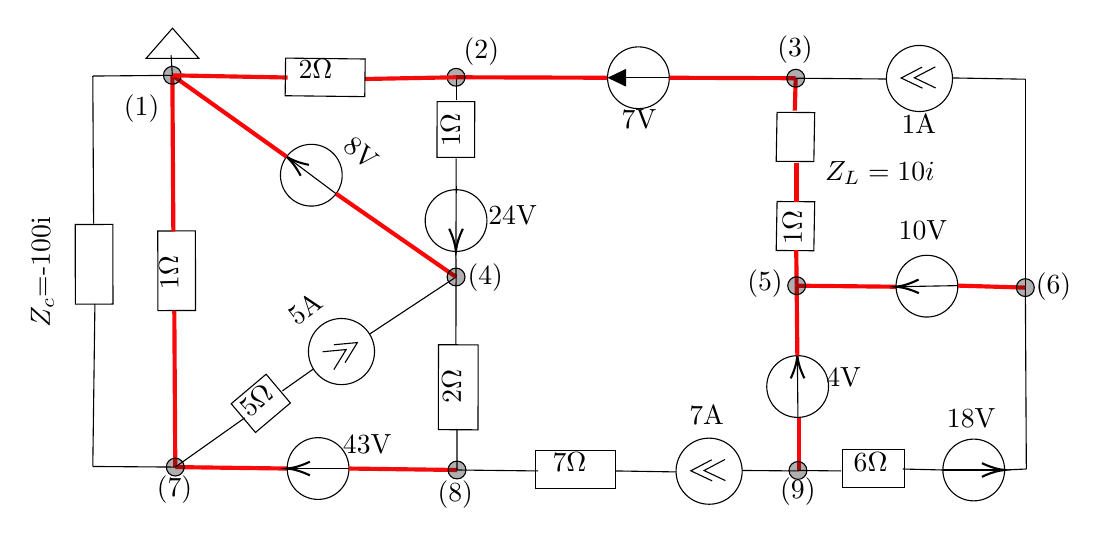
\begin{tikzpicture}[x=0.75pt,y=0.75pt,yscale=-1,xscale=1]
%uncomment if require: \path (0,441); %set diagram left start at 0, and has height of 441

%Flowchart: Connector [id:dp9270801755221227] 
\draw   (503.85,229.34) .. controls (503.85,221.12) and (510.51,214.46) .. (518.72,214.46) .. controls (526.94,214.46) and (533.6,221.12) .. (533.6,229.34) .. controls (533.6,237.55) and (526.94,244.21) .. (518.72,244.21) .. controls (510.51,244.21) and (503.85,237.55) .. (503.85,229.34) -- cycle ;
%Straight Lines [id:da6781562055832304] 
\draw    (503.85,229.34) -- (531.6,229.34) ;
\draw [shift={(533.6,229.34)}, rotate = 180] [color={rgb, 255:red, 0; green, 0; blue, 0 }  ][line width=0.75]    (10.93,-3.29) .. controls (6.95,-1.4) and (3.31,-0.3) .. (0,0) .. controls (3.31,0.3) and (6.95,1.4) .. (10.93,3.29)   ;

%Shape: Rectangle [id:dp34284039242623443] 
\draw   (455.5,219.58) -- (485.48,219.58) -- (485.48,237.71) -- (455.5,237.71) -- cycle ;
%Shape: Rectangle [id:dp04783594757199805] 
\draw   (143.72,114.15) -- (143.79,152.5) -- (125.66,152.53) -- (125.59,114.18) -- cycle ;
%Straight Lines [id:da23204009263337189] 
\draw [color={rgb, 255:red, 249; green, 7; blue, 7 }  ,draw opacity=1 ][line width=1.5]    (132.63,39.2) -- (133.1,114.51) ;
%Straight Lines [id:da7335986553607972] 
\draw [color={rgb, 255:red, 249; green, 10; blue, 10 }  ,draw opacity=1 ][line width=1.5]    (133.56,152.63) -- (134.03,227.94) ;
%Straight Lines [id:da7990553733639076] 
\draw [color={rgb, 255:red, 249; green, 9; blue, 9 }  ,draw opacity=1 ][line width=1.5]    (134.03,227.94) -- (187.95,228.64) ;
%Flowchart: Connector [id:dp40061918108006433] 
\draw   (217.71,228.64) .. controls (217.71,236.86) and (211.05,243.52) .. (202.83,243.52) .. controls (194.61,243.52) and (187.95,236.86) .. (187.95,228.64) .. controls (187.95,220.42) and (194.61,213.76) .. (202.83,213.76) .. controls (211.05,213.76) and (217.71,220.42) .. (217.71,228.64) -- cycle ;
%Straight Lines [id:da4449167399874583] 
\draw    (217.71,228.64) -- (189.95,228.64) ;
\draw [shift={(187.95,228.64)}, rotate = 360] [color={rgb, 255:red, 0; green, 0; blue, 0 }  ][line width=0.75]    (10.93,-3.29) .. controls (6.95,-1.4) and (3.31,-0.3) .. (0,0) .. controls (3.31,0.3) and (6.95,1.4) .. (10.93,3.29)   ;

%Straight Lines [id:da8855324753679816] 
\draw [color={rgb, 255:red, 244; green, 11; blue, 11 }  ,draw opacity=1 ][line width=1.5]    (269.77,229.34) -- (217.71,228.64) ;
%Straight Lines [id:da8796235187944343] 
\draw    (269.31,40.13) -- (269.31,51.29) ;
%Shape: Rectangle [id:dp3612475841800422] 
\draw   (278.31,51.89) -- (278.24,78.74) -- (260.11,78.69) -- (260.18,51.84) -- cycle ;
%Straight Lines [id:da95393971045362] 
\draw    (269.31,79.18) -- (269.38,94.29) ;
%Flowchart: Connector [id:dp9800044826411813] 
\draw   (269.38,94.29) .. controls (277.6,94.33) and (284.23,101.02) .. (284.19,109.24) .. controls (284.14,117.46) and (277.45,124.08) .. (269.23,124.04) .. controls (261.02,124) and (254.39,117.31) .. (254.43,109.09) .. controls (254.47,100.87) and (261.17,94.25) .. (269.38,94.29) -- cycle ;
%Straight Lines [id:da15518000296251477] 
\draw    (269.38,94.29) -- (269.24,122.04) ;
\draw [shift={(269.23,124.04)}, rotate = 270.29] [color={rgb, 255:red, 0; green, 0; blue, 0 }  ][line width=0.75]    (10.93,-3.29) .. controls (6.95,-1.4) and (3.31,-0.3) .. (0,0) .. controls (3.31,0.3) and (6.95,1.4) .. (10.93,3.29)   ;

%Shape: Rectangle [id:dp367367093472869] 
\draw   (160.97,197.41) -- (177.79,183.2) -- (189.49,197.05) -- (172.67,211.26) -- cycle ;
%Flowchart: Connector [id:dp8841244253872094] 
\draw   (200.58,180.68) .. controls (195.94,173.21) and (198.23,163.39) .. (205.7,158.75) .. controls (213.17,154.11) and (222.99,156.4) .. (227.63,163.87) .. controls (232.27,171.34) and (229.98,181.16) .. (222.51,185.8) .. controls (215.04,190.44) and (205.22,188.15) .. (200.58,180.68) -- cycle ;
\draw   (205.05,172.36) -- (216.36,171.31) -- (210.42,180.99) ;
\draw   (210.46,169) -- (221.77,167.95) -- (215.83,177.63) ;

%Straight Lines [id:da25407515856580676] 
\draw    (134.03,227.94) -- (167.5,204.23) ;
%Straight Lines [id:da13572938220558783] 
\draw    (200.58,180.68) -- (185.63,191.22) ;
%Straight Lines [id:da8309672731234929] 
\draw    (269.31,136.36) -- (227.63,163.87) ;
%Flowchart: Connector [id:dp5578065010047788] 
\draw   (211.5,96.22) .. controls (206.58,102.8) and (197.26,104.15) .. (190.68,99.23) .. controls (184.09,94.32) and (182.74,85) .. (187.66,78.41) .. controls (192.57,71.83) and (201.89,70.48) .. (208.48,75.4) .. controls (215.06,80.31) and (216.41,89.63) .. (211.5,96.22) -- cycle ;
%Straight Lines [id:da23421547181746738] 
\draw    (211.5,96.22) -- (189.26,79.61) ;
\draw [shift={(187.66,78.41)}, rotate = 36.75] [color={rgb, 255:red, 0; green, 0; blue, 0 }  ][line width=0.75]    (10.93,-3.29) .. controls (6.95,-1.4) and (3.31,-0.3) .. (0,0) .. controls (3.31,0.3) and (6.95,1.4) .. (10.93,3.29)   ;

%Straight Lines [id:da04123586462824069] 
\draw [color={rgb, 255:red, 249; green, 5; blue, 5 }  ,draw opacity=1 ][line width=1.5]    (132.63,39.2) -- (187.66,78.41) ;
%Straight Lines [id:da49872865252580456] 
\draw [color={rgb, 255:red, 249; green, 7; blue, 7 }  ,draw opacity=1 ][line width=1.5]    (211.5,96.22) -- (269.31,136.36) ;
%Straight Lines [id:da44523406254330533] 
\draw [color={rgb, 255:red, 247; green, 6; blue, 6 }  ,draw opacity=1 ][line width=1.5]    (269.31,40.13) -- (342.3,40.36) ;
%Flowchart: Connector [id:dp6481936777244088] 
\draw   (342.3,40.36) .. controls (342.3,32.15) and (348.96,25.48) .. (357.17,25.48) .. controls (365.39,25.48) and (372.05,32.15) .. (372.05,40.36) .. controls (372.05,48.58) and (365.39,55.24) .. (357.17,55.24) .. controls (348.96,55.24) and (342.3,48.58) .. (342.3,40.36) -- cycle ;
%Straight Lines [id:da5839724845528447] 
\draw    (345.3,40.36) -- (372.05,40.36) ;
\draw [shift={(342.3,40.36)}, rotate = 0] [fill={rgb, 255:red, 0; green, 0; blue, 0 }  ][line width=0.08]  [draw opacity=0] (8.93,-4.29) -- (0,0) -- (8.93,4.29) -- cycle    ;
%Straight Lines [id:da4086201601102246] 
\draw [color={rgb, 255:red, 241; green, 8; blue, 8 }  ,draw opacity=1 ][line width=1.5]    (372.05,40.36) -- (432.95,40.59) ;
%Straight Lines [id:da9907410146063771] 
\draw    (308.82,229.8) -- (269.77,229.34) ;
%Shape: Rectangle [id:dp4109210949540476] 
\draw   (307.66,220.04) -- (346.02,220.04) -- (346.02,238.17) -- (307.66,238.17) -- cycle ;
%Straight Lines [id:da28996442195871497] 
\draw    (375.31,230.27) -- (346.48,229.8) ;
%Flowchart: Connector [id:dp7851498713964808] 
\draw   (407.14,229.57) .. controls (407.34,238.36) and (400.37,245.64) .. (391.58,245.84) .. controls (382.78,246.03) and (375.5,239.06) .. (375.31,230.27) .. controls (375.11,221.48) and (382.08,214.19) .. (390.88,214) .. controls (399.67,213.81) and (406.95,220.78) .. (407.14,229.57) -- cycle ;
\draw   (399.06,234.45) -- (388.79,229.59) -- (398.84,224.29) ;
\draw   (392.69,234.59) -- (382.42,229.73) -- (392.47,224.43) ;

%Straight Lines [id:da46869741115925057] 
\draw    (434.34,229.8) -- (407.14,229.57) ;
%Straight Lines [id:da3419614768986434] 
\draw [color={rgb, 255:red, 247; green, 7; blue, 7 }  ,draw opacity=1 ][line width=1.5]    (434.34,204.23) -- (434.34,229.8) ;
%Flowchart: Connector [id:dp2681269475222585] 
\draw   (434.02,204) .. controls (425.8,204.08) and (419.08,197.48) .. (419,189.26) .. controls (418.93,181.05) and (425.53,174.33) .. (433.74,174.25) .. controls (441.96,174.17) and (448.68,180.77) .. (448.76,188.99) .. controls (448.83,197.2) and (442.23,203.93) .. (434.02,204) -- cycle ;
%Straight Lines [id:da46089558980747936] 
\draw    (434.02,204) -- (433.76,176.25) ;
\draw [shift={(433.74,174.25)}, rotate = 89.47] [color={rgb, 255:red, 0; green, 0; blue, 0 }  ][line width=0.75]    (10.93,-3.29) .. controls (6.95,-1.4) and (3.31,-0.3) .. (0,0) .. controls (3.31,0.3) and (6.95,1.4) .. (10.93,3.29)   ;

%Straight Lines [id:da7816849807429227] 
\draw [color={rgb, 255:red, 249; green, 6; blue, 6 }  ,draw opacity=1 ][line width=1.5]    (433.41,140.54) -- (433.74,174.25) ;
%Straight Lines [id:da3718856473883132] 
\draw [color={rgb, 255:red, 246; green, 7; blue, 7 }  ,draw opacity=1 ][line width=1.5]    (432.95,40.59) -- (432.5,56.19) ;
%Shape: Rectangle [id:dp8576529816284628] 
\draw   (442.1,100.11) -- (441.68,123.7) -- (423.55,123.58) -- (423.97,99.99) -- cycle ;
%Straight Lines [id:da31094674347815277] 
\draw [color={rgb, 255:red, 247; green, 6; blue, 6 }  ,draw opacity=1 ][line width=1.5]    (433.41,140.54) -- (433.2,123.41) ;
%Straight Lines [id:da3869535881571553] 
\draw    (432.95,40.59) -- (476.65,40.97) ;
%Flowchart: Connector [id:dp17553917091137916] 
\draw   (508.49,40.45) .. controls (508.64,49.24) and (501.63,56.48) .. (492.84,56.63) .. controls (484.04,56.78) and (476.8,49.77) .. (476.65,40.97) .. controls (476.51,32.18) and (483.52,24.94) .. (492.31,24.79) .. controls (501.1,24.64) and (508.35,31.65) .. (508.49,40.45) -- cycle ;
\draw   (500.38,45.28) -- (490.14,40.37) -- (500.21,35.12) ;
\draw   (494.01,45.39) -- (483.77,40.48) -- (493.85,35.23) ;

%Straight Lines [id:da22633949871034376] 
\draw    (508.49,40.45) -- (543.59,41.06) ;
%Straight Lines [id:da3167725086528861] 
\draw    (543.59,41.06) -- (543.59,141.47) ;
%Straight Lines [id:da8368926936960823] 
\draw [color={rgb, 255:red, 247; green, 6; blue, 6 }  ,draw opacity=1 ][line width=1.5]    (481.3,141.05) -- (433.41,140.54) ;
%Flowchart: Connector [id:dp6624088763704992] 
\draw   (511.05,140.51) .. controls (511.2,148.72) and (504.66,155.5) .. (496.44,155.65) .. controls (488.23,155.8) and (481.45,149.26) .. (481.3,141.05) .. controls (481.15,132.83) and (487.69,126.05) .. (495.9,125.9) .. controls (504.12,125.75) and (510.9,132.29) .. (511.05,140.51) -- cycle ;
%Straight Lines [id:da5732322951082511] 
\draw    (511.05,140.51) -- (483.3,141.01) ;
\draw [shift={(481.3,141.05)}, rotate = 358.96] [color={rgb, 255:red, 0; green, 0; blue, 0 }  ][line width=0.75]    (10.93,-3.29) .. controls (6.95,-1.4) and (3.31,-0.3) .. (0,0) .. controls (3.31,0.3) and (6.95,1.4) .. (10.93,3.29)   ;

%Straight Lines [id:da5331520742576463] 
\draw [color={rgb, 255:red, 251; green, 9; blue, 9 }  ,draw opacity=1 ][line width=1.5]    (511.05,140.51) -- (543.59,141.47) ;
%Straight Lines [id:da4718092007885628] 
\draw    (434.02,229.57) -- (454.8,229.8) ;
%Straight Lines [id:da7629795316134069] 
\draw    (503.85,229.34) -- (484.55,228.87) ;
%Straight Lines [id:da49460765952991026] 
\draw    (543.59,141.47) -- (544.06,228.87) ;
%Straight Lines [id:da8663012236530663] 
\draw    (533.6,229.34) -- (544.06,228.87) ;
%Shape: Ellipse [id:dp9599988863799103] 
\draw  [fill={rgb, 255:red, 13; green, 12; blue, 12 }  ,fill opacity=0.33 ] (128.33,39.2) .. controls (128.33,36.82) and (130.26,34.9) .. (132.63,34.9) .. controls (135.01,34.9) and (136.93,36.82) .. (136.93,39.2) .. controls (136.93,41.57) and (135.01,43.5) .. (132.63,43.5) .. controls (130.26,43.5) and (128.33,41.57) .. (128.33,39.2) -- cycle ;
%Shape: Ellipse [id:dp4291349974742562] 
\draw  [fill={rgb, 255:red, 13; green, 12; blue, 12 }  ,fill opacity=0.33 ] (265.01,40.13) .. controls (265.01,37.75) and (266.93,35.83) .. (269.31,35.83) .. controls (271.68,35.83) and (273.61,37.75) .. (273.61,40.13) .. controls (273.61,42.5) and (271.68,44.43) .. (269.31,44.43) .. controls (266.93,44.43) and (265.01,42.5) .. (265.01,40.13) -- cycle ;
%Shape: Ellipse [id:dp35514614123372956] 
\draw  [fill={rgb, 255:red, 13; green, 12; blue, 12 }  ,fill opacity=0.33 ] (265.01,136.36) .. controls (265.01,133.99) and (266.93,132.06) .. (269.31,132.06) .. controls (271.68,132.06) and (273.61,133.99) .. (273.61,136.36) .. controls (273.61,138.74) and (271.68,140.66) .. (269.31,140.66) .. controls (266.93,140.66) and (265.01,138.74) .. (265.01,136.36) -- cycle ;
%Shape: Ellipse [id:dp4574714015140131] 
\draw  [fill={rgb, 255:red, 13; green, 12; blue, 12 }  ,fill opacity=0.33 ] (129.73,227.94) .. controls (129.73,225.57) and (131.65,223.64) .. (134.03,223.64) .. controls (136.4,223.64) and (138.33,225.57) .. (138.33,227.94) .. controls (138.33,230.32) and (136.4,232.24) .. (134.03,232.24) .. controls (131.65,232.24) and (129.73,230.32) .. (129.73,227.94) -- cycle ;
%Shape: Ellipse [id:dp9460605223558882] 
\draw  [fill={rgb, 255:red, 13; green, 12; blue, 12 }  ,fill opacity=0.33 ] (265.47,229.34) .. controls (265.47,226.96) and (267.4,225.04) .. (269.77,225.04) .. controls (272.15,225.04) and (274.07,226.96) .. (274.07,229.34) .. controls (274.07,231.71) and (272.15,233.64) .. (269.77,233.64) .. controls (267.4,233.64) and (265.47,231.71) .. (265.47,229.34) -- cycle ;
%Shape: Ellipse [id:dp5338988376316147] 
\draw  [fill={rgb, 255:red, 13; green, 12; blue, 12 }  ,fill opacity=0.33 ] (428.65,40.59) .. controls (428.65,38.22) and (430.58,36.29) .. (432.95,36.29) .. controls (435.32,36.29) and (437.25,38.22) .. (437.25,40.59) .. controls (437.25,42.97) and (435.32,44.89) .. (432.95,44.89) .. controls (430.58,44.89) and (428.65,42.97) .. (428.65,40.59) -- cycle ;
%Shape: Ellipse [id:dp417109854685058] 
\draw  [fill={rgb, 255:red, 13; green, 12; blue, 12 }  ,fill opacity=0.33 ] (429.11,140.54) .. controls (429.11,138.17) and (431.04,136.24) .. (433.41,136.24) .. controls (435.79,136.24) and (437.72,138.17) .. (437.72,140.54) .. controls (437.72,142.92) and (435.79,144.84) .. (433.41,144.84) .. controls (431.04,144.84) and (429.11,142.92) .. (429.11,140.54) -- cycle ;
%Shape: Ellipse [id:dp23473344672881535] 
\draw  [fill={rgb, 255:red, 13; green, 12; blue, 12 }  ,fill opacity=0.33 ] (429.72,229.57) .. controls (429.72,227.2) and (431.64,225.27) .. (434.02,225.27) .. controls (436.39,225.27) and (438.32,227.2) .. (438.32,229.57) .. controls (438.32,231.95) and (436.39,233.87) .. (434.02,233.87) .. controls (431.64,233.87) and (429.72,231.95) .. (429.72,229.57) -- cycle ;
%Shape: Ellipse [id:dp7107280358371015] 
\draw  [fill={rgb, 255:red, 13; green, 12; blue, 12 }  ,fill opacity=0.33 ] (539.29,141.47) .. controls (539.29,139.1) and (541.22,137.17) .. (543.59,137.17) .. controls (545.97,137.17) and (547.89,139.1) .. (547.89,141.47) .. controls (547.89,143.85) and (545.97,145.77) .. (543.59,145.77) .. controls (541.22,145.77) and (539.29,143.85) .. (539.29,141.47) -- cycle ;
%Straight Lines [id:da8762375608574078] 
\draw [color={rgb, 255:red, 246; green, 11; blue, 11 }  ,draw opacity=1 ][line width=1.5]    (132.63,39.2) -- (188.19,40.25) ;
%Straight Lines [id:da19933192741177086] 
\draw [color={rgb, 255:red, 242; green, 12; blue, 12 }  ,draw opacity=1 ][line width=1.5]    (225.44,40.96) -- (269.31,40.13) ;
%Straight Lines [id:da23885940688338092] 
\draw    (269.74,209.48) -- (269.77,229.34) ;
%Shape: Rectangle [id:dp41568117043171604] 
\draw   (279.96,169.07) -- (279.88,209.99) -- (260.77,209.9) -- (260.84,168.98) -- cycle ;
%Straight Lines [id:da24256258147812892] 
\draw    (269.23,168.75) -- (269.31,136.36) ;
%Straight Lines [id:da8005810494074346] 
\draw    (269.23,124.04) -- (269.31,136.36) ;
%Shape: Rectangle [id:dp6974751057127131] 
\draw   (187.18,30.89) -- (225.53,31.33) -- (225.32,49.46) -- (186.97,49.02) -- cycle ;
%Straight Lines [id:da25243416376340266] 
\draw    (132.63,39.2) -- (94.29,39.54) ;
%Straight Lines [id:da15632893684713278] 
\draw    (94.29,39.54) -- (94.68,110.65) ;
%Straight Lines [id:da6024318707517089] 
\draw    (95.31,149.25) -- (94.29,227.64) ;
%Shape: Rectangle [id:dp9688324081815436] 
\draw   (103.95,111.03) -- (104.01,149.39) -- (85.88,149.42) -- (85.82,111.06) -- cycle ;

%Straight Lines [id:da9377650456468498] 
\draw    (94.29,227.64) -- (134.03,227.94) ;
%Shape: Rectangle [id:dp5011504866273262] 
\draw   (442.1,57.14) -- (441.68,80.74) -- (423.55,80.62) -- (423.97,57.02) -- cycle ;
%Straight Lines [id:da4909204796526594] 
\draw [color={rgb, 255:red, 246; green, 7; blue, 7 }  ,draw opacity=1 ][line width=1.5]    (433.34,100.06) -- (433.34,81.38) ;
%Shape: Triangle [id:dp6830309231688889] 
\draw   (132.69,16.5) -- (145.38,31) -- (120,31) -- cycle ;
%Straight Lines [id:da39919615469560776] 
\draw    (132.63,39.2) -- (132,29.5) ;

% Text Node
\draw (185.31,152.7) node [anchor=north west][inner sep=0.75pt]  [rotate=-322.88] [align=left] {5A};
% Text Node
\draw (213.55,211.19) node [anchor=north west][inner sep=0.75pt]   [align=left] {43V};
% Text Node
\draw (220.16,65.62) node [anchor=north west][inner sep=0.75pt]  [rotate=-41.03] [align=left] {8V};
% Text Node
\draw (283.63,100.78) node [anchor=north west][inner sep=0.75pt]   [align=left] {24V};
% Text Node
\draw (347.87,54.29) node [anchor=north west][inner sep=0.75pt]   [align=left] {7V};
% Text Node
\draw (380.41,197.01) node [anchor=north west][inner sep=0.75pt]   [align=left] {7A};
% Text Node
\draw (446.43,178.88) node [anchor=north west][inner sep=0.75pt]   [align=left] {4V};
% Text Node
\draw (504.57,198.41) node [anchor=north west][inner sep=0.75pt]   [align=left] {18V};
% Text Node
\draw (481.33,107.99) node [anchor=north west][inner sep=0.75pt]   [align=left] {10V};
% Text Node
\draw (482.69,56.85) node [anchor=north west][inner sep=0.75pt]   [align=left] {1A};
% Text Node
\draw (125.31,143.94) node [anchor=north west][inner sep=0.75pt]  [rotate=-268.74] [align=left] {1\ohm};
% Text Node
\draw (162,197.65) node [anchor=north west][inner sep=0.75pt]  [rotate=-318.32] [align=left] {5\ohm};
% Text Node
\draw (260.94,75.05) node [anchor=north west][inner sep=0.75pt]  [rotate=-269.34] [align=left] {1\ohm};
% Text Node
\draw (314.56,219.79) node [anchor=north west][inner sep=0.75pt]   [align=left] {7\ohm};
% Text Node
\draw (425.51,121.99) node [anchor=north west][inner sep=0.75pt]  [rotate=-270.09] [align=left] {1\ohm};
% Text Node
\draw (459.61,219.56) node [anchor=north west][inner sep=0.75pt]   [align=left] {6\ohm};
% Text Node
\draw (108.02,47.33) node [anchor=north west][inner sep=0.75pt]   [align=left] {(1)};
% Text Node
\draw (271.71,19.89) node [anchor=north west][inner sep=0.75pt]   [align=left] {(2)};
% Text Node
\draw (422.8,18.73) node [anchor=north west][inner sep=0.75pt]   [align=left] {(3)};
% Text Node
\draw (273.57,128.91) node [anchor=north west][inner sep=0.75pt]   [align=left] {(4)};
% Text Node
\draw (408.39,131.7) node [anchor=north west][inner sep=0.75pt]   [align=left] {(5)};
% Text Node
\draw (547.39,133.09) node [anchor=north west][inner sep=0.75pt]   [align=left] {(6)};
% Text Node
\draw (123.88,230.72) node [anchor=north west][inner sep=0.75pt]   [align=left] {(7)};
% Text Node
\draw (259.16,233.27) node [anchor=north west][inner sep=0.75pt]   [align=left] {(8)};
% Text Node
\draw (424.2,231.88) node [anchor=north west][inner sep=0.75pt]   [align=left] {(9)};
% Text Node
\draw (261.27,198.54) node [anchor=north west][inner sep=0.75pt]  [rotate=-270.58] [align=left] {2\ohm};
% Text Node
\draw (192.2,30.44) node [anchor=north west][inner sep=0.75pt]   [align=left] {$\displaystyle 2\si{\ohm}$};
% Text Node
\draw (445.83,79.54) node [anchor=north west][inner sep=0.75pt]   [align=left] {$\displaystyle Z_{L} =10i$};
% Text Node
\draw (63.18,161.86) node [anchor=north west][inner sep=0.75pt]  [rotate=-270.16] [align=left] {$\displaystyle Z_{c}$=-100i};


\end{tikzpicture}

\end{center}

\newpage
\begin{thebibliography}{15}
\bibitem{math}
Mathcha \href{https://www.mathcha.io/}{https://www.mathcha.io/} Pentru desenarea circuitelor

\bibitem{ciup}
G. Ciuprina, D. Ioan, M. Popescu, A.S. Lup, R. B˘arbulescu, \emph{Teoria circuitelor electrice.
Seminar}, disponibil pe moodle.

\bibitem{dan}
Daniel Ioan, \emph{Circuite electrice rezistive - breviare teoretice ¸si probleme},
\href{http://www.lmn.pub.ro/ daniel/culegere.pdf}{http://www.lmn.pub.ro/ daniel/culegere.pdf}, 2000.

\bibitem{refer}
Gabriela Ciuprina Template pentru redactarea rapoartelor in LaTeX (v5) \href{http://www.lmn.pub.ro/ gabriela/LatexTemplate4Students/}{http://www.lmn.pub.ro/ gabriela/LatexTemplate4Students/}
\end{thebibliography}
\end{document}


